%%%%%%%%%%%%%%%%%%%%%%%%%%%%%%%%%%%%%%%%%%%%%%%%%%%%%%%%%%%%%%%%%%%%%%%%%%%%%%%
% template.tex - version 0.9.1.1 (5/26/2011)
%
% This is a template file for the osudiss-2 class. See
% osudiss-2.pdf for documentation, and the GS material 
% for the requirements.
%
% Copy the following osudiss-2 files your latex path (or just the folder containing this file):
% osudiss-2.cls (v0.9.1)
% sa-draftwater.sty
%
% Then, to compile this file:
% latex template
% bibtex template
% latex template
% latex template
%
% (You can also use pdflatex if you prefer.)
%
%%%%%%%%%%%%%%%%%%%%%%%%%%%%%%%%%%%%%%%%%%%%%%%%%%%%%%%%%%%%%%%%%%%%%%%%%%%%%%%
\documentclass[11pt, double, phd]{osudiss-2} 
% The `11pt' option is unnecessary since it is the default

% `onehalf' sets the line spacing to one-and-a-half spacing instead of
% double spacing.

% The `phd' option is unnecessary since it is the default

% Remove `draft' option for final draft

%%%%%%%%%%%%%%%%%%%%%%%%% Packages %%%%%%%%%%%%%%%%%%%%%%%%%
% Load your favorite packages here
\usepackage{graphicx} % for importing images in figures - you definitely want this!
\usepackage{lipsum} % for fake latin text---you probably don't want this
\usepackage{verbatimbox}

% For instance... see osudiss-2.pdf for some suggestions, if you don't
% have a clue
\usepackage{bm} % for bold math---useful
\usepackage{booktabs} % for more professional tables
\usepackage[titletoc]{appendix}

%hyperref packages and options
\usepackage{bookmark} % helps booksmarks look better in PDF
%hypersetup option 'breaklinks' is reguired for line wrapping in the table of contents during latex compilation, and can be removed if you use pdflatex
%\hypersetup{colorlinks=true,linkcolor=blue, breaklinks} %internal links in blue, citations in green
\hypersetup{colorlinks=true,linkcolor=black, citecolor=black, urlcolor=black, breaklinks} %all links in black
\usepackage[all]{hypcap}

%Use of natbib is STRONGLY recommended to sort and compress your references within each citation
%With these options, natbib will convert i.e. [5,3,9,4] to [3-5, 9]
\usepackage[sort&compress]{natbib}

%required to have latex automatically generate subfigures (i.e. (a), (b) etc)
\usepackage{subfig}
\usepackage[export]{adjustbox}
\setcounter{lofdepth}{2}
\PassOptionsToPackage{obeyspaces}{url}
%\usepackage{hyperref}% http://ctan.org/pkg/hyperref

%load glossaries packages
\usepackage[acronym, section=chapter]{glossaries}
%\usepackage[xindy,acronym, section=chapter]{glossaries} %- recommended if supported by your OS
\makeglossaries %required to actually make a glossary
\include{acronyms} %load list of acronyms contained in acronyms.tex

%The following commands can be used to help deal with "overfull hbox" issues
%See, for example, http://www.tex.ac.uk/cgi-bin/texfaq2html?label=overfull for details
%\pretolerance 1000
\setlength{\emergencystretch}{3em}
%\tolerance 1000

%%%%%%%%%%%%%%%%%%%%%%%%% Custom Commands/Environments %%%%%%%%%%%%%%%%%%%%%%%%%
% Put your favorite custom commands here
\newcommand{\fish}{\alpha} % some of my students call it the "fish" symbol

%Print list of abbreviations - use same font as List of Figures and List of Tables for the title, and same formatting in the table of contents.
% Argument #1 - title for list of abbreviations (i.e. List of Abbreviations)

\newcommand\PrintListofAbbreviations[1]{
	\phantomsection
	\addcontentsline{toc}{front}{\typesetColumnHeading{#1}}
	\printglossary[type=\acronymtype,title={\protect {\typesetLevelTwo{#1}}}]
}


\newenvironment{chapabstract}{%
	\begin{center}%
		\bfseries Abstract
\end{center}}%

% Below is an example of customizing the style of headings in your
% dissertation. See osudiss-2.pdf for more information.
%
% For example, if you simply must have uppercase titles:
%\renewcommand\typesetLevelOne[1]{{\Large\textbf{\MakeUppercase{#1}}\par}}
%\renewcommand\typesetLevelTwo[1]{{\Large\textbf{\MakeUppercase{#1}}}}
% Note the \par for \typesetLevelOne
%
% If you want the title to be bold and |\Large| instead of |\Huge|:
%\renewcommand\titleFont{\normalfont\Large\bfseries}

% Add words that TeX may not know how to hyphenate below. This can
% help prevent overfull hboxes. For example,
\hyphenation{eigen-state space-time} 

%%%%%%%%%%%%%%%%%%%%%%%%% Document Metadata %%%%%%%%%%%%%%%%%%%%%%%%%
\title{High-Accuracy Atomic Calculations for Plasma Opacities}
\degree{Doctor of Philosophy} % Default value
\author{Lianshui Zhao}
\advisorname{Chris Orban}
\member{Anil Pradhan, Co-Advisor}
\member{Amy Connolly}
\member{Enam Chowdhury}
\authordegrees{M.Sc.}
\graduationyear{2019}
\unit{Graduate Program in Physics} 

\newcommand\ion[2]{#1$\;${\scshape{#2}}}
\usepackage{multirow}
%replace the "Figure 1.:" with "Figure 1. figure_caption". The same as for tables.
\DeclareCaptionLabelFormat{mylabel}{#1 #2.\hspace{1ex}}
\captionsetup[figure]{labelformat=mylabel,labelsep=none,name=Figure}
\captionsetup[table]{labelformat=mylabel,labelsep=none,name=Table}

%\usepackage{subcaption}
%fix the figure format 1a to 1(a)
%\usepackage[labelformat=simple]{subcaption}
%\usepackage{subfigure}
%\renewcommand\thesubfigure{(\alph{subfigure})}
\graphicspath{{chap_6/}{chap_5/}{chap_4/}{chap_3/}{chap_2/}{chap_1/}{app_2/}}
\robustify{\subref} %replace \protect\subfig{}
\usepackage{amsfonts} %mathbb

\setcounter{secnumdepth}{4} %section 1.1.1.1
\setcounter{tocdepth}{4} %create headings 1.1.1.1

\renewcommand{\arraystretch}{1.3} %increase the spacing betwen rows in tables.
\usepackage{lscape} 
\usepackage{amsmath}
%-----------------------------------------------------%
%%%                    BODY 		     		%%%
%-----------------------------------------------------%
%\includeonly{chap_6/topup_bprm_rdw} %useful when editing large document by only processing the the chapters you are interested in.
%\includeonly{app_1/app_1}
%\includeonly{chap_5/pec_l_edge}
%\includeonly{chap_3/bprm_rdw_theory}
%\includeonly{app_2/bprm_code}
%\includeonly{chap_4/bprm_fe17_fe18}
%\includeonly{chap_2/Introduction}
%\includeonly{abstract/abstract}
%\includeonly{acknowledge/acknowledgement}
%\includeonly{vita/vita}
\usepackage{xcolor} %colorbox{gray!20}

%modified version of cases by placing the brace on the right.
\newenvironment{rcases}
{\left.\begin{aligned}}
	{\end{aligned}\right\rbrace}

\begin{document}
\frontmatter 

\begin{abstract}
	Rosseland mean opacity of the solar elemental composition is a required input microphysics in the standard solar model. The opacity table used two decades ago contributed to the excellent agreement between the standard solar model and the helioseismology measurement. However, more realistic stellar atmosphere modeling suggested a drastic reduction in the solar metallicity, which caused significant discrepancies in many aspects of the Sun between the standard solar model and the helioseismology. To restore the agreement, some authors argue that the opacities should be larger. There is some experimental evidence for this. Iron opacity measured at the conditions similar to those near the solar convection zone base using the Sandia National Laboratories Z facility revealed significant underestimation of the opacity by all available theoretical models. 
	
	With the goal of obtaining more accurate Rosseland Mean Opacity we carry out the ab-initio atomic calculations for radiative data using the state-of-the-art codes including a close-coupling Breit-Pauli $R$-Matrix code and a relativistic distorted wave code. With the supercomputing power we have today, we are able to do the largest-scale Breit-Pauli $R$-Matrix calculation for \ion{Fe}{xvii} and \ion{Fe}{xviii}. To ensure the completeness and convergence of the data, we use the relativistic distorted wave calculation to ``top up" the $R$-Matrix data, and a detailed description of bridging the $R$-Matrix calculation and relativistic distorted wave calculation is presented in this dissertation.

\end{abstract}

\dedication{Dedicated to my family and Shaoyun Dong.\\
						 \vspace{10 mm}
						\includegraphics[width=.5\textwidth]{shaoyun_dong}}
					
\begin{acknowledgments}
	First of all, I would like to thank the not-too-bad China-U.S. relations over the past few years. I believe if there is a problem, there is always a GOOD way out of it. No matter who will lead the world, I hope both countries and all others can get along well with each other, till the end of the time.
	
	I would like to thank the Physics Department of the Ohio State University (OSU) for offering me an excellent opportunity to work on my Ph.D. degree in this great department, full of wonderful people and brilliant minds. Heartful thanks go to Jon Pelz and Kris Dunlap for their support and help especially during the time after I quit from Dr. Yang's condensed matter experimental group and before I joined the computational group that I am in now. I also would like to thank all the people who make this department great.
	
	My sincere thanks are due to Anil Pradhan for accepting me who had almost no computational experience as a group member, having me work on projects that helped me gain lots of programming experience, and providing one academic travel and one summer GRA financial support. I also would like to thank him and Sultana Nahar for their teaching on the atomic physics and the relevant code. I am also very grateful for Chris Orban, who gave me a quick start at the beginning of my computational research, helped me a great deal in programming, and always tried to be helpful throughout my Ph.D career. Among my Ph.D. committee, I would like to thank Amy Hill and Enam Chowdhury for their care and attention paied in my progress towards the completion of my degree. I'm also extremely grateful for Werner Eissner for his well-maintained $R$-Matrix code and for his help in fixing one fatal bug. Without him, I do not think I would make this far, and the whole project might fail. I also quite enjoyed working with him, though remotely.
	
	I would like to thank David Heisterberg at the Ohio Supercomputer Center (OSC), who helped me a lot in providing lots of information when my PBS jobs failed, especially at the beginning of $R$-Matrix calculation leading to the discovery that ``scratch'' files in Fortran consume memory at OSC, thus the a-few-hundred-GB-memory problem is resolved. I also would like to thank David Will in the Astronomy Department of OSU, especially for his kind and generosity in allocating more computing resources to my PBS jobs for a few months just before Arjuna cluster was retired. I also would like to thank Keith Stewart and Sandy Shew for their helpful guidance in leveraging ASC Unity cluster and for doubling the active PBS jobs I can have.
	
	Special thanks go to the following friends and colleagues who helped me run the large-scale $R$-Matrix calculation using their Unity computing resources (names in alphabetic order): Jiaxin Wu, Keng Yuan Meng, Max Westphal, Xiankun Li, Yonas Getachew and Zhefu Yu, without whose help I could never finish the work as planned.
	
	At last, I would love to thank my family for their constant support in the past six years and thank Shaoyun Dong for appearing in my life, accompanying me for the past more than a year, and helping me concentrate on the important things in my life. I hope you and I can spend the rest of our lives together, till the end of the time.
	
\end{acknowledgments}
\begin{vita}
\dateitem{Apr. 02, 1990}{Born---Suqian, China}
\dateitem{July, 2013}{B.S., Changchun University of Science and Technology, Changchun, Jilin, China}
\dateitem{Dec., 2015}{M.S., The Ohio State University, Columbus, OH, USA}
% Insert other relevant items here (GTA, etc.)

\begin{publist}
\pubitem{``Converged R-Matrix Calculation of the Photoionization of \ion{Fe}{xvii} in Astrophysical Plasmas: from Convergence to Completeness''  Lianshui Zhao, Werner Eissner, Sultana Nahar, and Anil Pradhan 2018, ASP Conf. Ser., 515, 89}

\pubitem{``Contribution from Ising domains overlapping out-of-plane to perpendicular magnetic anisotropy in Mn4N thin films on MgO(001)'' Andrew Foley, Joseph Corbett, Alam Khan, Andrea L. Richard, David C. Ingram, Arthur R. Smith, Lianshui Zhao, James C.
Gallagher, Fengyuan Yang 2017, J. Magn. Magn. Mater., 439, 236}

\end{publist}


\begin{fieldsstudy}
\majorfield{Physics}
\onestudy{Atomic Physics}{Pradhan-Orban's group} % optional
% Alternatively you can do:
\end{fieldsstudy}

\end{vita}

\tableofcontents
 
% list of figures (comment out if you don't have any figures)
\clearpage %remove if you don't want a page break before list of figures
\listoffigures 

% list of tables (comment out if you don't have any tables)
\clearpage  %remove if you don't want a page break before list of tables
\listoftables 


\mainmatter
\include{chap_2/Introduction}
\chapter{Close Coupling $R$-Matrix Theory and Distorted Wave Theory}
\label{chap_bprm_rdw_theory}

\section{Introduction}
The suites of codes that are used in my current work to generate the atomic radiative data, i.e. oscillator strength and photoionization cross section, were developed initially for solving the electron-ion collision problems. One difference between the processes involved in photoionization and electron collision is the projectile, i.e. photons for photoionization and electrons for electron collision. However, they do share the similar final process, i.e. a system consisting of a final target ion and an outgoing electron. Thus these packages used in electron collision problems were extended to calculate the radiative data, for example Opacity Project \citep{opcd_1, opcd_2} and Iron Project \citep{ip_1}. Depending on how the coupling among channels is treated, the methodologies can be separated into two categories, one considers the coupling, i.e. close coupling approximation, and the other neglects such coupling completely, which simplifies into a single-channel problem, i.e. distorted wave approximation. In close coupling approximation, there are several approaches to the electron-ion collision problems, i.e. solving the coupled integro-differential equations, such as IMPACT \citep{impact_3, impact_1, impact_2}, $R$-Matrix \citep{rm_1, rm_2, rm_3}, etc., which solve the same physical problems, only differring by the numerical techniques used in these packages. And a comparision between these two packages can be found in \citet{comp_impact_rm}. In the distorted wave approximation, which is based on the assumption that the coupling between channels is weak, coupled integro-differential equations reduce to a single-channel differential equation, and a good review on different versions of this approximation can be found in \citet{dw_review_1}.

In the following section, solving the coupled integro-differential equations is outlined using close coupling approximation $R$-Matrix approach and distorted wave approximation. As the atomic nuclear charge $Z$ increases, the relativistic effects become more and more important, thus for low-$Z$ elements, non-relativistic treatment is enough, but for medium- and high-$Z$ atoms/ions, relativistic effect has to be included. Therefore, in the above two approximations, non-relativistic and relativistic versions of them are discussed.

\section{Collision Theory -- Solving the Coupled Integro-Differential Equations}
The electron-ion collision problem can be described by the time-independent Schr\"odinger equation
\begin{equation} \label{eq_schodinger}
	H^{N+1}\Psi = E\Psi
\end{equation}
where $E$ is the total energy of the ion + electron system. The Hamiltonian of the system in atomic units is 
\begin{equation} \label{eq_hamiltonian}
	H^{N+1} = \sum_{n=1}^{N=1} (-\frac{1}{2}\nabla_n^2-\frac{Z}{r_n}+\sum_{m>n}^{N+1}\frac{1}{r_{nm}})
\end{equation}
where the first two terms denote the one-electron term, while the last one two-electron term, $r_n$ is the distance between the electron and the nucleus with atomic number $Z$, and $r_{nm} = |\textbf{r}_n-\textbf{r}_m|$ is the  inter-electron distance in which $\textbf{r}_n$ is the vector drawn from the nucleus. The relativistic effects are neglected for the time being. The eigen-wavefunction $\psi_k$ can be expanded in terms of a set of $N$-electron target wavefunctions $\Phi$ and the wavefunction of the colliding electron $\theta$
\begin{align}
	\psi_k(x_1\cdot\cdot\cdot x_{N+1}) &= \mathcal{A}\sum_{i}\Phi_i(x_1\cdot\cdot\cdot x_{N})\theta_i(x_{N+1}) \label{wave_expand}\\
	\theta_i(x) &=Y_{li}^{m_{li}}(r)\delta(m_{si}|\sigma)\frac{1}{r}F_i(r)
\end{align}
where $k$ characterizes the initial conditions and usually denotes the collision channel, $\mathcal{A}$ is antisymmetrization operator, $x_n$ denotes the space and spin coordinates of the nth electron, $Y_l^m$ is a sphyerical harmonic, $\sigma$ is a spin coordinate, $F_i(r)$ describes the radial part of the colliding electron. The target state $\Phi_i$ can be written as a configuration interaction expansion in terms of some basis configurations $\phi_i$ by
\begin{equation} \label{eq_target_expand}
	\Phi_i(x_1\cdots x_N) = \sum_kb_{ik}\phi_k(x_1\cdots x_N)
\end{equation}
where the configuration mixing coefficients $b_{ik}$ are determined by diagonalizing the target Hamiltonian in the basis of $\phi_k$. The target Hamiltonian is defined by equation \ref{eq_hamiltonian} with $N+1$ replaced by $N$ and the energy of state $\Phi_i$ is defined by
\begin{equation} \label{eq_dia_target}
	\langle\Phi_i|H^N|\Phi_j\rangle=E_i^N\delta_{ij}
\end{equation}
The configurations $\phi_i$ are constructed from a bound orbital basis consisting of self consistent field orbitals plus some additional pseudo-orbitals included to model electron correlation effect. The expansion of $\Phi_i$ in the basis of $\phi_k$ is just like the Slater determinant, which treats fully the antisymmetric requirement of the wavefunctions for a system of fermions. The radial parts of these one-electron orbitals, $P_{nl}(r)$, satisfy the orthonormality conditions 
\begin{equation}
	\langle P_{n_il}|P_{n_jl} \rangle = \int_{0}^{\infty} P_{n_il}(r)P_{n_jl}(r)dr=\delta_{n_in_j}
\end{equation}
The radial functions $P_{nl}(r)$ are provided externally from other atomic structure packages, e.g. SUPERSTRUCTURE \citep{ss_1, ss_2, ss_3}, and a brief description of SUPERSTRUCTURE can be found in Appendix \ref{app_bprm_code}. 

Pincipally the target states $\Phi_i$ included in the expansion are complete, however, in practice they are included partly with the ones of interest. And expansion \ref{wave_expand} can be rewritten in the following form
\begin{multline} \label{eq_full_expand}
	\psi_k(x_1\cdot\cdot\cdot x_{N+1}) = \mathcal{A}\sum_{i}^{n}\overline{\Phi}_i(x_1\cdot\cdot\cdot x_{N}; \hat{\textbf{r}}_{N+1}\sigma_{N+1}) \frac{1}{r_{N+1}} F_{ik}(r_{N+1}) \\+ \sum_{j=1}^m d_{jk} \chi_j(x_1\cdots x_{N+1}) 
\end{multline}
where $n$ is the number of channels; $\overline{\Phi}_i$ is the channel function, which is obtained by coupling the target state $\Phi_i$ with the angular and spin functions of the colliding electron to form the total angular momentum and parity, $F_{ik}$ is the radial component of the colliding electron wavefunction and called channel orbitals, and $\chi_j$ is the $(N+1)$-electron bound state function, which is formed by the one-electron atomic wavefunctions. To allow for fast convergence numerically, an orthogonality condition is usually required for $l_i = l_j$
\begin{equation} \label{eq_bound_free_orth}
	\langle P_{n_jl_j}|F_{ik}\rangle = \int_{0}^{\infty}P_{n_jl_j}(r)F_{ik}(r)dr=0
\end{equation}
, in which case the second term in equation \ref{eq_full_expand} has to be introduced, serving two purposes. Part of the states included in the second term are to ensure the completeness of the expansion of the target-electron wavefunctions. In the electron-ion collision problem, the colliding electron can be free after collision, or can be captured by the target. The orthogonality condition of equation \ref{eq_bound_free_orth} means the radial wavefunction of the colliding electron projects out of the subshell space of the target, which can be interpreted as keeping the colliding electron from being captured into any incomplete subshells, and this phenomenon is described in the first term of the expansion \ref{eq_full_expand}. It represents a free channel expansion, because the channel orbitals $F_{ik}$ can be freely varied. To be complete, the fact that the colliding electron can be captured by the target needs to be addressed, which is exactly what the second term in expansion \ref{eq_full_expand} describes, i.e. an $(N+1)$-electron system with one-electron atomic wavefunctions for all electrons and these states are constructed using the same target radial functions $P_{nl}$. And this term is called correlation functions, representing the bound channel expansion. And the other states included in the second term of equation \ref{eq_full_expand} is to allow for improved description of short-range electron correlation effects. To elaborate on how to choose the $(N+1)$-electron bound channel configurations, for example, if $Ck_jl_j$ represents a free channel term, where $C$ denotes the target state configuration, then after imposing the orthogonality condition, it is necessary to include in the second term a bound channel configuration $Cnl$. More examples can be found in \citet{dw_review_1, henry_1993}. To solve for the channel orbitals $F_i(r)$, we can substitute wavefunction \ref{eq_full_expand} into Sch\"odinger equation \ref{eq_schodinger}, project onto the channel functions $\overline\Phi_i$ and functions $\chi_j$, separte out the spin and angular variables and eliminate the coefficients $d_{jk}$, and finally obtain the following set of coupled integro-differential equations \citep{bspline_2006}
\begin{equation} \label{eq_coupled_intdiff}
	\Bigg(\frac{d^2}{dr^2} - \frac{l_i(l_i+1)}{r^2} + \frac{2Z}{r} + k_i^2\Bigg) F_i(r) = 2 \sum_j(V_{ij}+W_{ij}+X_{ij})F_j(r)
\end{equation}
where $l_i$ is the orbital angular momentum of the colliding electron, $V_{ij},~W_{ij}$ and $X_{ij}$ are the partial-wave decompositions of the local direct, non-local exchange and non-local correlation potentials, whch generally are too complicated to write down explicitely. This equation is the core of electron-ion collision theory, and close coupling approximation considers such coupling and exchange terms, while distored wave approximation neglects them. In the following section, these two approximations are outlined.

\subsection{$R$-Matrix Approach}
To solve the coupled integro-differential equation \ref{eq_coupled_intdiff}, \citet{rm_1} developed the $R$-Matrix approach, which starts by dividing the configuration sapce into two regions, i.e. internal region and external region. See figure \ref{figure_rm_space}. When the colliding electron interacts with the target ion, in the internal region, the electron is indistinguishable from the other electrons belonging to the target ion, while in the external region, it is far away from these target electrons and explicitly distinguishable. Thus, in the internal region, instead of solving the coupled integro-differential equations, we can treat the $(N+1)$-electron wavefunction as an expansion of an energy-independent basis set, just like the $N$-electron target, including the exchange and other correlation effects. In the external region, electron exchange and correlation effects between the target and the colliding electron can be neglected if the $R$-Matrix boundary is chosen large enough that the charge distribution of the target is contained within the sphere, and this can be guaranteed by the radial part of the target wavefunciton being negligibly samll. However, the channel orbitals $F_i(r=a)$ should be non-zero, which provides a link between the solution in the internal and external regions.

%======= FIGURE: 
\begin{figure}
	\centering
	\includegraphics[width=.9\textwidth]{figures_3/r_matrix_box}	
	\caption{The partition of the configuration space in $R$-Matrix approach.}
	\label{figure_rm_space}
\end{figure}

In section \ref{sec_nr_rm}, the procedure of solving for the channel orbitals in internal and external regions will be outlined, which closely follows \citet{rm_3}, and this is the non-relativistic version of $R$-Matrix approach. In section \ref{sec_r_rm}, the relativistic effects \citep{rm_2} are included in the Hamiltonian and the difference from the non-relativistic version is discussed.

\subsubsection{Non-Relativistic} \label{sec_nr_rm}
In the internal region, the target wavefunctions are expanded as in equation \ref{eq_target_expand}, but the basis of the channel orbitals needs to be determined. Practically the basis $u_{ij}(r)$ satisfying the following single-channel scattering equation is adopted
\begin{equation} \label{eq_single_channel}
	\Bigg(\frac{d^2}{dr^2} - \frac{l_i(l_i+1)}{r^2} + V_0(r) + k_{ij}^2\Bigg) u_{ij}(r) = \sum_{n=1}^{NRANG2} \Lambda_{ijn} P_{nl_i}(r)
\end{equation}
with the boundary conditions
\begin{equation} \label{eq_boundary_condition}
	\begin{split}
		u_{ij}(0) &= 0 \\
		\Bigg(\frac{a}{u_{ij}(a)} \Bigg) \Bigg(\frac{du_{ij}}{dr} \Bigg)_{r=a} &=b
	\end{split}
\end{equation}
where $NRANG2$ is the number of continuum basis included in the calculation; the Lagrange multipliers $\Lambda_{ijn}$ ensure the continuum basis orthogonal to the bound orbitals $P_{nl_i}(r)$ of the same angular symmetry; the potential $V_0(r)$ behaves like $\frac{2Z}{r}$, which is not crucial; $k_{ij}^2$ is the energy of the colliding electron in $Ry$; b is arbitrary, and is normally set to 0. An algorithm about generating such basis can be found in \citet{cont_orbital}.

The continuum basis $u_{ij}(r)$ is orthogonal to both themselves and the bound orbitals within the $R$-Matrix boundary $r=a$
\begin{equation}
	\begin{split}
		(u_{ij}|u_{ij'}) &= 0\\
		(u_{ij}|P_{nl_i}) &= 0
	\end{split}
\end{equation}
where the round brackets indicate the integration range is from 0 to a. Since the bound orbitals $P_{nl_i)}(r)$ is orthoganal to the channel orbital $F_i(r)$ in the whole range and $P_{nl_i}(r>a)$ is negligibly small, thus it is equivalent to $(u_{ij}|P_{nl_i}) = 0$.

Therefore for each channel i, a complete set of basis is formed within $R$-Matrix boudary
\begin{equation}
	P_{n_{min}l_i}, \cdots, P_{n_{max}l_i}, u_{i1}, u_{i2}, \cdots, u_{i NRANG2}
\end{equation}
where $n_{min} = l_i+1$, and the total eigen-wavefunction $\psi_k$ can be expanded in such basis, independent of the total energy $E$. Thus equation \ref{eq_full_expand} can be rewritten as
\begin{multline} \label{eq_full_expand_cont_basis}
	\psi_k(x_1\cdot\cdot\cdot x_{N+1}) = \mathcal{A}\sum_{i=1}^{n}\sum_{j=1}^{NRANG2}c_{ijk}\overline{\Phi}_i(x_1\cdot\cdot\cdot x_{N}; \hat{\textbf{r}}_{N+1}\sigma_{N+1}) \frac{1}{r_{N+1}} u_{ij}(r_{N+1}) \\+ \sum_{j=1}^m d_{jk} \chi_j(x_1\cdots x_{N+1}) 
\end{multline}
where $c_{ijk}$ and $d_{ik}$ can be determined by diagonalizing 
\begin{equation} \label{eq_diag_np1}
	(\psi_k|H^{N+1}|\psi_{k'}) = E_k\delta_{kk'}
\end{equation}

The total wavefunction of $(N+1)$-electron system within $R$-Matrix boundary can be expanded as 
\begin{equation}
	\Psi = \sum_k A_{EK} \psi_k
\end{equation}
where $A_{EK}$ is the coefficient that is energy independent. Define
\begin{equation}
	\frac{1}{r}w_{ik}(r) = \sum_j c_{ijk}u_{ij}(r) = (\overline{\Phi}_i|\psi_k)
\end{equation}
and the reduced radial wavefunction of the colliding electron
\begin{equation}
	\frac{1}{r}F_i(r) = \frac{1}{r} \sum_k A_{EK} w_{ik}(r) = (\overline{\Phi}_i|\Psi)
\end{equation}
It can be shown that $A_{EK}$ can be written as the following form
\begin{equation}
	A_{EK} = \frac{1}{2a} (E_k-E)^{-1} \sum_i w_{ik}(a) \Bigg( a\frac{dF_i}{dr} - bF_i \Bigg)_{r=a}
\end{equation}

\begin{equation} \label{eq_rm_a}
	F_i(a) = \sum_j R_{ij}(E) \Bigg( a\frac{dF_j}{dr} - bF_j \Bigg)_{r=a}
\end{equation}
where $R$-Matrix is defined as 
\begin{equation} \label{eq_rm_boundary}
	R_{ij}(E) = \frac{1}{2a} \sum_k \frac{w_{ik}(a)w_{jk}(a)}{E_k - E}
\end{equation}
The surface amplitude $w_{ik}(a)$ and poles $E_k$ are obtained directly from the eigenvectors and eigenvalues of the Hamiltonian matrix defined in equation \ref{eq_diag_np1}. And $R$-matrix is obtained for all energies by diagonalizing $H^{N+1}$ once for each symmetry, and this is the advantage of $R$-Matrix method when computing at numerious energies, especially in the resonance region. The reduced radial wavefunction $F_i(a)$ is to be matched with the solution in the external region.

As the summation in equation \ref{eq_rm_boundary} is truncated to some finite number of terms, the other distant, neglected terms can play an important role in the diagonal elements of the $R$-matrix where they add coherently. These neglected terms can be included by solving the differential equation
\begin{equation}
\Bigg(\frac{d^2}{dr^2} - \frac{l_i(l_i+1)}{r^2} + V_0(r) + k_{i}^2\Bigg) u_{i}^0(r) = \sum_{k} \Lambda_{ijk} P_k(r)
\end{equation}
, which is the same as equation \ref{eq_single_channel}, but is solved at channel energies $k_i^2$ without applying the boundary condition equations \ref{eq_boundary_condition} at $r=a$. Suppose the $R$-Matrix is calculated from the first $N$ terms in the continuum expansion, the correction to the diagonal elements of the $R$-Matrix at the energy $k_i^2$ is 
\begin{equation}
	\begin{split}
		R_{ii}^c (N, k_i^2) &\approx \frac{1}{a} \sum_{j=N+1}^{\infty} \frac{u_{ij}(a)^2}{k_{ij}^2-k_i^2} \\
		& = \Bigg[ \frac{a}{u_i^0(a)} \Bigg( \frac{du_i^0}{dr} \Bigg)_{r=a} -b \Bigg]^{-1} - \frac{1}{a} \sum_{j=1}^{N} \frac{u_{ji}(a)^2}{k_{ij}^2 - k_i^2}
	\end{split}
\end{equation}
, where $u_{ij}(r)$ refers to the jth eigensolution of equation \ref{eq_single_channel} with the boundary condition, and $u_i^0$ is the solution without boundary condition. We therefore use the corrected $R$-Matrix in place of equation \ref{eq_rm_boundary}
\begin{equation}
R_{ij}(E) = \frac{1}{2a} \sum_k \frac{w_{ik}(a)w_{jk}(a)}{E_k - E} +R_{ii}^c(N, k_i^2)\delta_{ij}
\end{equation}

At this point the theoretical methods applied in the internal region is described, and we are to solve the integro-differential equations \ref{eq_coupled_intdiff} in the external region, in which the exchange and correlation terms can be neglected, thus the total wavefunction can be written as 
\begin{equation} \label{eq_new_expand}
	\Psi(x_1\cdot\cdot\cdot x_{N+1}) = \sum_{i}^{n}\overline{\Phi}_i(x_1\cdot\cdot\cdot x_{N}; \hat{\textbf{r}}_{N+1}\sigma_{N+1}) \frac{1}{r_{N+1}} F_{i}(r_{N+1}) 
\end{equation}
where $\overline{\Phi}_i$ are the same as those used in the internal region, but with no exchange between the target electrons and the colliding electron. After substituting equation \ref{eq_new_expand} into Schr\"odinger equation and projecting onto the channel functions, we obtain the following coupled differential equations
\begin{equation}
\Bigg(\frac{d^2}{dr^2} - \frac{l_i(l_i+1)}{r^2} +\frac{2Z}{r} + k_{i}^2\Bigg) F_{i}(r) = 2\sum_{j=1}^n V_{ij} F_j(r)
\end{equation}
, which can be reduced to
\begin{equation}\label{eq_ex_diff}
	\Bigg(\frac{d^2}{dr^2} - \frac{l_i(l_i+1)}{r^2} +\frac{2(Z-N)}{r} + k_{i}^2\Bigg) F_{i}(r) = 2\sum_{\lambda=1}^{\lambda_{max}} \sum_{j=1}^{n} \frac{a_{ij}^\lambda}{r^{\lambda+1}} F_j(r) 
\end{equation}
, where $n$ is the number of channels in the expansion, $l_i$ and $k_i^2$ are the channel angular momenta and energies, $N$ is the number of electron in the target, $a_{ij}^\lambda$ is the long-range potential coefficients. In BPRM code (see Appendix \ref{app_bprm_code}), such long-range multipole potentials on the right hand side of equation \ref{eq_ex_diff} is treated with two options. One is to neglect (IPERT = 0) them, and the other is to treat them as a perturbation (IPERT = 1) with $\lambda = 1,~2$ \citep{opcd_2}.

The asymptotic form of the channel orbitals $F_i(r)$ at infinity is
\begin{equation} \label{eq_f_asymptotic}
	F_{ij}(r) \underset{r \to \infty}{\sim}
	\begin{cases}
		k_i^{-1/2}(sin\theta_i\delta_{ij}+cos\theta_iK_{ij}), & \text{open~channels} \\
		exp(-\phi_i)\delta_{ij}, & \text{close~channels}
	\end{cases}
\end{equation}
, where the second index $j$ on $F_{ij}$ denotes the linearly independent solutions of equation \ref{eq_ex_diff}, and 
\begin{align}
	\theta_i &= k_ir-\frac{1}{2}l_i\pi-\eta_iln2k_ir+arg\Gamma (l_i+1+i\eta _i) \label{eq_theta}\\
	\eta_i &= -\frac{z}{k_i} \\
	\phi_i &= |k_i|r - \frac{z}{|k_i|}ln (2|k_i|r) \label{eq_phi}
\end{align}
, where $z=Z-N$ is the residual target charge.

In principle, we can integrate equation \ref{eq_ex_diff} outwards subject to the $R$-matrix boundary condition of equations \ref{eq_rm_a}, and fit to the asymptotic form of equation \ref{eq_f_asymptotic}, however, the open channel solution is not fully determined until the reactance matrix $K$ in equation \ref{eq_f_asymptotic} is found.

When calculating the radiative data, i.e. oscillator strength and photoioization cross section, we need the wavefunctions of bound states (all channels are closed) and free states (at least one channel is open), thus at this point where we have discussed the techniques used in the internal and external regions, we are ready to link the solutions in these two regions.

To find the solution for the bound states, we can define $n$ linearly  independent solutions of the external region equation \ref{eq_ex_diff}, which satisfy the following boundary condition
\begin{equation}
	c_{ij}(r) \underset{r \to \infty}{\sim} exp(-\phi_i)\delta_{ij} \qquad i = 1,n \quad j = 1, n
\end{equation}
, where $\phi_i$ is given by \ref{eq_phi}. We can expand external solution in terms of those solutions
\begin{equation}
	F_i(r) = \textbf{cx} = \sum_{j=1}^n c_{ij}(r)x_j \qquad i = 1,n 
\end{equation} 
, where $x_j$ can be determined by substituting this expression for $F_i$ into the interal wavefunction at the boundary $r=a$
\begin{equation} \label{eq_frmb}
	\mathbf{F} = a\textbf{R} \cdot \dot{\mathbf{F}} - b \mathbf{R} \cdot \mathbf{F}
\end{equation}
, where $\dot{\mathbf{F}} = d\mathbf{F}/dr$. We get the following $n$ homogeneous equations 
\begin{equation}
	\mathbf{cx} = a \mathbf{R\dot{c}x} - b \mathbf{Rcx}
\end{equation}
Solving for $\mathbf{x}$ with nontrivial solutions, we find the condition is 
\begin{equation}
	\text{det}~ \mathbf{B} = 0
\end{equation}
, where $\mathbf{B} = \mathbf{c} - a \mathbf{R}(\dot{\mathbf{c}}- \frac{b}{a}\mathbf{c})$, thus the wavefunctions and energy levels for the bound states are solved.

To find the solutions for the free states, a similar method as for the bound states can be adopted. In this case, we introduce $(n+n_a)$ linearly independent solutions $s_{ij}(r)$ and $c_{ij}(r)$ of equation \ref{eq_ex_diff}, satisfying the following boundary conditions
\begin{equation}
	\begin{rcases}
		s_{ij}(r) \\
		c_{ij}(r) \\
		c_{ij}(r) \\
	\end{rcases}
	\underset{r \to \infty}{\sim} 
	\begin{cases}
	sin\theta_i\delta_{ij} 	& i=1,n \qquad j = 1,n_a\\
	cos\theta_i\delta_{i, j-n_a} & i=1,n \qquad j = 1,n_a\\
	exp(-\phi_i)\delta_{i,j-n_a} & i=1,n \qquad j = n_a+1,n \\
	\end{cases}
\end{equation}
, where $\theta_i$ and $\phi_i$ are defined as \ref{eq_theta} and \ref{eq_phi}, respectively. Thus the reduced radial wavefunction $F_{ij}(r)$ can be expanded as
\begin{equation}
	\mathbf{F=s+cK}
\end{equation}
After substituting it into equation \ref{eq_frmb} and solving for $\mathbf{K}$, we have
\begin{equation}
	\mathbf{K=B^{-1}A}
\end{equation}
, where $\mathbf{A} = -\mathbf{s} +a\mathbf{R}(\dot{\mathbf{s}}-\frac{b}{a}\mathbf{s})$, $\mathbf{B} = \mathbf{c} +a\mathbf{R}(\dot{\mathbf{c}}-\frac{b}{a}\mathbf{c})$. Thus the entire wavefunctions of the free states are solved.


\subsubsection{Relativistic} \label{sec_r_rm}
For medium heavy element like iron, the relativistic effects should be included and the Breit-Pauli Hamiltonian is sufficient, which results from the reduction of the Dirac equation and Breit interaction to Pauli form \citep{rm_2, scott_bprm}. The Breit-Pauli Hamiltonian can be written as
\begin{equation}
	H_{BP}^{N+1} = H_{NR}^{N+1} + H_{REL}^{N+1} 
\end{equation}
, where $H_{NR}^{N+1}$ is defined as equation \ref{eq_hamiltonian}, and $H_{REL}^{N+1}$ consists of the one-body operators that are given by 
\begin{subequations}
	\begin{align}
		H_{mass}^{N+1} &= -\frac{1}{8}\alpha^2 \sum_{i=1}^{N+1} \nabla_i^4 \qquad \text{the mass-correction term}\\
		H_D^{N+1} &= -\frac{1}{8}\alpha^2 Z \sum_{i=1}^{N+1} \nabla_i^4 (\frac{1}{r_i}) \qquad \text{the one-body Darwin term}\\
		H_{SO}^{N+1} &= \frac{1}{2}\alpha^2 Z \sum_{i=1}^{N+1} \frac{1}{r_i^3} (\mathbf{l}_i\cdot \mathbf{S}_i) \qquad \text{the spin-orbit interaction}
	\end{align}
\end{subequations}
$H_{NR}^{N+1},~H_{mass}^{N+1} and H_D^{N+1}$ commute with $\mathbf{L}^2$, $\mathbf{S}^2$, $\mathbf{L}_Z$,  $\mathbf{S}_Z$ and parity, while $H_{BP}^{N+1}$ only commutes with $\mathbf{J}^2$, $\mathbf{J}_Z$ and parity.

This difference in the Hamiltonian from the non-relativistic version of $R$-Matrix theory affects several aspects of the Breit-Pauli $R$-Matrix theory. One is in the diagonalization of equations \ref{eq_dia_target} and \ref{eq_diag_np1} , where the Breit-Pauli Hamiltonian is used. And the angular coupling scheme is changed to $jK$ pair coupling
\begin{equation}
	\mathbf{J}_i +\mathbf{l} = \mathbf{K} \qquad \mathbf{K+\frac{1}{2}=J}
\end{equation}
, where $J_i$ is the total angular momentum of the target state. And this results in a much larger Hamiltonian matrix, which requires considerably more computational effort. The rest of the method is the same as the non-relativistic version.



\subsection{Distorted Wave Approximation}
In this section, a much simpler approximation than the close coupling is discussed. We will briefly introduce the non-relativistic distorted wave approximation, followed by a more detailed fully relativistic distorted wave approximation, which is mainly about the techniques used in flexible atomic code (FAC) \citep{gu_2008}.
\subsubsection{Non-Relativistic}
In the distorted wave approximation, the coupling, exchange and correlation potentials on the right hand side of the integro-differential equation \ref{eq_coupled_intdiff} are neglected. Thus with the non-relativistic Hamiltonian, it reduces to a single-channel differential equation \citep{book_int_diff}
\begin{equation}
\Bigg(\frac{d^2}{dr^2} - \frac{l_i(l_i+1)}{r^2} +V_i(r) + k_{i}^2\Bigg) f_{i}(r) = 0
\end{equation}                    
, where $V_i(r)\underset{r \to \infty}{\sim} \frac{2(Z-N)}{r}$. And the boundary condition for $f_i(r)$ is
\begin{subequations}
	\begin{align}
		f_i(0) &= 0 \\
		f_i(r) &\underset{r \to \infty}{\sim} k_i^{-1/2}sin\Bigg( k_ir+\frac{z}{k_i}lnr+\tau_i \Bigg)
	\end{align}
\end{subequations}
With the solutions $f_i(r)$, we construct functions
\begin{equation}
	F_i = f_i - \sum_{\alpha}\delta(l_i, l_\alpha)(f_i|P_\alpha)P_\alpha
\end{equation}
, which satisfy the orthogonality conditions
\begin{equation}
	(F_i|P_\alpha) = 0 \qquad  \text{if} \quad l_i= l_\alpha
\end{equation}
Since the channel coupling is neglected, the radial functions with the boundary condition $i'$ are 
\begin{equation}
	F_{ii'} = F_i \delta_{ii'}
\end{equation}
Thus the coupled expansion \ref{eq_full_expand} can be rewritten as
\begin{multline} \label{eq_full_expand_dw}
	\psi_i(x_1\cdot\cdot\cdot x_{N+1}) = \mathcal{A}\overline{\Phi}_i(x_1\cdot\cdot\cdot x_{N}; \hat{\textbf{r}}_{N+1}\sigma_{N+1}) \frac{1}{r_{N+1}} F_{i}(r_{N+1}) \\+ \sum_{j=1}^m d_{j} \chi_j(x_1\cdots x_{N+1}) 
\end{multline}
Since the current calculation does not use the non-relativistic distorted wave approximation, we will not spend more effort on this topic, more information can be found in \citet{ucl_dw}.


\subsubsection{Relativistic}
The fully relativistic distorted wave code we use is FAC (flexible atomic code), which is developed by Ming Feng Gu \citep{gu_2008}, who applied many of the techniques that were used in the existing code at that time \citep{dw_guoxin, dw_sampson, dw_zhang, hullac}, wrote the code from scratch and made the package available to public. FAC treats the bound and continuum processes altogether, and is very efficient in computing various atomic quantities. In the rest of the section, the methods used for solving for the bound and continuum wavefunctions are described.

The many-electron Dirac Hamiltonian is 
\begin{equation}
	H = \sum_{i=1}^N H_D(i) +\sum_{i<j}^N \frac{1}{r_{ij}}
\end{equation}
, where $N$ is the number of electrons in the atomic system, $H_D(i)$ is the single-electron Dirac Hamiltonian for the potential due to the nuclear charge. The wavefunction of the system can be expanded as
\begin{equation}
	\psi = \sum_\nu b_\nu \Phi_\nu
\end{equation}
, where $b_\nu$ is the coefficients by diagonalizing the total Hamiltonian, $\Phi_\nu$ are the configuration state functions, which are antisymmetric sums of the products of $N$ one-electron Dirac spinors $\varphi_{n\kappa m}$
\begin{equation}
	\varphi_{n\kappa m} = \frac{1}{r}
	\begin{pmatrix}
		P_{n\kappa} (r) \chi_{\kappa m}(\theta, \phi, \sigma) \\
		iQ_{n\kappa} (r) \chi_{-\kappa m}(\theta, \phi, \sigma)
	\end{pmatrix}
\end{equation}
, where $P_{n\kappa}$ and $Q_{n\kappa}$ are the large and small components of the radial function; $\chi_{\kappa m}$ is the usual spin-angular function; $n$ is the principle quantum number; $\kappa$ is the relativistic angular quantum number, which is related to the orbital and total angular momentum by
\begin{equation}
	\kappa = (l-j)(2j+1)
\end{equation}
and $m$ is the $z$-component of the total angular momentum $j$. 

For bound states, the one-electron large and small components,  $P_{n\kappa}$ and $Q_{n\kappa}$, satisfy the following coupled Dirac equations
\begin{equation} \label{eq_dirac_eq}
	\begin{split}
		\Bigg( \frac{d}{dr} + \frac{\kappa}{r} \Bigg) P_{n\kappa} &= \alpha \Bigg( \varepsilon_{n\kappa} - V + \frac{2}{\alpha ^2} \Bigg) Q_{n\kappa} \\
		\Bigg( \frac{d}{dr} - \frac{\kappa}{r} \Bigg) Q_{n\kappa} &= \alpha \Bigg( - \varepsilon_{n\kappa} + V \Bigg) P_{n\kappa}
	\end{split}
\end{equation}
, where $\alpha$ is fine structure constant in atomic unit, and $\varepsilon_{n\kappa}$ are the energy eigenvalues of the raidal functions. The local central potential $V$ includes the contribution from the nuclear charge $V^N(r)$ and the electron-electron interaction $V^{ee}(r)$. The nuclear potential is 
\begin{equation}
	V^N = 
	\begin{cases}
		\frac{Z}{2}\Big(\frac{4}{R_N}\Big)\Big[3-\Big(\frac{r}{R_N}\Big)^2\Big], \qquad & r \leq R_N \\
		Z, & r > R_N
	\end{cases}
\end{equation}
, where $R_N$ is the statistical model radius of the nucleus, which can be expressed in terms of the atomic number $A$, $R_N = 2.2677\times10^{-15}A^{1/3}$. The electron-electron interaction excluding the self-interaction term is 
\begin{multline}
	V^{ee}(r) = \frac{1}{r\sum_a\omega _a\rho _a(r)} \Bigg\{ \sum_{ab} \omega_a(\omega_{ab}-\delta_{ab})Y_{bb}^0(r) \rho_a(r) \\+ \sum_a \omega_a(\omega_a-1)\sum_{k>0} f_k(a, a) Y_{aa}^k(r)\rho_a(r) + \sum_{a \neq b} \sum_k \omega_a \omega_b g_k(a, b)Y_{ab}^k(r) \rho_{ab}(r) \Bigg\}
\end{multline}
, where $a=n\kappa$ and $b=n'\kappa'$ denote the subshells; $\omega_a$ and $\omega_b$ the occupation number of subshells $a$ and $b$, which are usually called mean configuration and about half an electron is excited, and 
\begin{equation}
	\begin{split}
		\rho_{ab} = P_a(r) P_b(r) + Q_a(r) Q_b(r) \\
		Y_{ab}^k(r) = r \int \frac{r_<^k}{r_>^{k+1}} \rho_{ab} (r') dr'
	\end{split}
\end{equation}
, where $r_<$ and $r_>$ are the lesser and greater of $r$ and $r'$, respectively. $f_k$ and $g_k$ are the direct and exchange coefficients defined as 
\begin{equation}
	\begin{split}
		f_k(a, b) &= -
						\Bigg( 1+\frac{1}{2j_a} \Bigg)
						\binom{~~j_a \qquad k \qquad j_b}{-\frac{1}{2} \qquad 0 \qquad \frac{1}{2}} ^2  \\
		g_k(a, b) &= - \binom{~~j_a \qquad k \qquad j_b}{-\frac{1}{2} \qquad 0 \qquad \frac{1}{2}}^2
	\end{split}
\end{equation}
The orthonomality condition satisfied by the bound radial functions is 
\begin{equation} \label{eq_bound_orth}
	\int_0^\infty dr [P_{n\kappa}(r)P_{n'\kappa}(r) + Q_{n\kappa}(r)Q_{n'\kappa}(r)] = \delta_{nn'}
\end{equation}
To solve the coupled Dirac equations \ref{eq_dirac_eq}, we can eliminate the small component and define the following variables
\begin{equation}
	\begin{split}
		P_a &= \xi_a(r) F_a(r) \\
		\xi_a(r) &= \sqrt{1+\frac{\alpha^2}{2}[\varepsilon_a-V(r)]} \\
		Q_a &= \frac{\alpha}{2\xi_a^2} \Bigg( \frac{d}{dr} P_a + \frac{\kappa}{r} P_a \Bigg)
	\end{split}
\end{equation}
, and we have the following equation
\begin{equation} \label{eq_rdw_f}
	\frac{d^2}{dr^2}F_a(r) + \Bigg\{ 2[\varepsilon_a - U(r)] - \frac{\kappa (\kappa+1)}{r^2} \Bigg\}F_a(r) =0
\end{equation}
, where 
\begin{equation}
	\begin{split}
		U(r) &= V(r) - \frac{\alpha^2}{2} \Bigg \{ [V(r)-\varepsilon_a]^2 - W(r) \Bigg\} \\
		W(r) &= \frac{1}{4\xi^2(r)} \Bigg [ \frac{d^2}{dr^2}V(r) + \frac{3\alpha^2}{4\xi^2(r)}\Bigg( \frac{d}{dr} V(r)\Bigg)^2 - \frac{2\kappa}{r} \frac{d}{dr} V(r)\Bigg]
	\end{split}
\end{equation}
After a further transformation with
\begin{equation}
	\begin{split}
		t = t(r) \\
		F_a(r) = \Bigg( \frac{dt}{dr} \Bigg)^{-1/2}G_a(t)
	\end{split}
\end{equation}
, equation \ref{eq_rdw_f} can be transformed into
\begin{multline} \label{eq_rdw_f_final}
	\frac{d^2}{dt^2}G_a(t) = \Bigg( \frac{dt}{dr}\Bigg)^{-2} G_a(t) \Bigg\{ \frac{\kappa(\kappa+1)}{r^2} - 2[\varepsilon_a - U(r)] + \frac{1}{2}\Bigg( \frac{dt}{dr}\Bigg)^{-1} \frac{d^3t}{dr^3} \\ - \frac{3}{4} \Bigg( \frac{dt}{dr}\Bigg)^{-2} \Bigg( \frac{d^2t}{dr^2}\Bigg)^2	\Bigg\}
\end{multline}
With the boundary conditions of zero-amplitude at both ends, we can use the Numerov method to integrate equation \ref{eq_rdw_f_final} both outward and inward and match at the outer classical turning point. The $r$ range is $(10^{-6}/z, 500/z)$, where $z$ is the residul target charge, and the mesh used is of the form $c_1\sqrt{t}+c_2ln(r)$.

For the continuum radial wavefunction, it is very similar to that described for bound states, but with a few differences. The Dirac equation \ref{eq_dirac_eq} is replaced by
\begin{equation}
\begin{split}
\Bigg( \frac{d}{dr} + \frac{\kappa}{r} \Bigg) P_{\epsilon\kappa} &= \alpha \Bigg( \varepsilon_{\epsilon\kappa} - V + \frac{2}{\alpha ^2} \Bigg) Q_{\epsilon\kappa} \\
\Bigg( \frac{d}{dr} - \frac{\kappa}{r} \Bigg) Q_{\epsilon\kappa} &= \alpha \Bigg( - \varepsilon_{\epsilon\kappa} + V \Bigg) P_{\epsilon\kappa}
\end{split}
\end{equation}
, where $\epsilon$ is positive and is the kinetic energy of the electron in atomic units. The orthonomality condition \ref{eq_bound_orth} is replaced by
\begin{equation} 
\int_0^\infty dr [P_{\epsilon\kappa}(r)P_{\epsilon'\kappa}(r) + Q_{\epsilon\kappa}(r)Q_{\epsilon'\kappa}(r)] =\pi \delta(\epsilon - \epsilon')
\end{equation}
In the inner region, where the wavefunction is not oscillatory or the oscillation period is large enough to contain sufficient number of grid points, we use the Numerov method to integrate the equation outward, and in the rest of the region, the phase-amplitude method is used. The inner and outer solutions are matched at the region interface by requiring the continuity of $F(r)$ and its first derivative.

\section{Conclusion}
In this chapter, the methods of close coupling $R$-Matrix and distorted wave are discribed to solve the integro-differential equations, and the former includes the channel coupling, exchange and correlation potentials and is very computationally expensive, while the latter neglects them all and is very fast and efficient as implemented in FAC package. With these sovled wavefunctions, we are ready to calculate the atomic radiative data, which is the focus of Chapter \ref{chap_bprm_fe17_fe18}.







\chapter{BPRM Calculations for \ion{Fe}{XVII} and \ion{Fe}{XVIII}}
\label{chap_bprm_fe17_fe18}

\section{Formulae for Radiative Quantities}
The opacity calculation needs weighted oscillator strength data due to bound-bound transitions and photoionization cross section data due to bound-free transitions \citep{opcd_1}. For bound-bound transitions, the monochromatic opacity is 
\begin{equation}
	\kappa_\omega (a \to b) = \frac{2\pi^2e^2}{mc} N_af(b, a)\phi_\omega
\end{equation}
, where $\omega = 2\pi \nu$ is the angular frequency, $N_a$ is the total number of ions $X^{a+}$ per unit volume, $f(b, a)$ is the oscillator strength, $\phi_\omega$ is a profile factor normalized to
\begin{equation}
	\int \phi_\omega d\omega = 1
\end{equation}
The weighted oscillator strength is 
\begin{equation}
	g_af(b,a) = \frac{2m}{e^2\hbar} \omega_0\frac{\mathbf{S}(b; a)}{3}
\end{equation}
, where $g_a$ is the statistical weight of the initial bound state and $\textbf{S}$ is the line strength
\begin{equation}
	\mathbf{S}(b; a) = | (b||\mathbf{D}||a) |^2
\end{equation}
, where $\mathbf{D}$ is 
\begin{equation}
	\mathbf{D} = e \sum_n \mathbf{r}_n
\end{equation}
, where $\mathbf{r}_n$ is the coordinate of an ionic electron and the sum is over all electrons in the ion.
For bound-free transitions, the monochromatic opacity is
\begin{align}
	\kappa_\omega (a \to E'f) &= \frac{N_a}{g_a} \frac{4\pi^2}{3c} \omega \mathbf{S}(E'f; a) \\
	 & = N_a \sigma_\omega(a \to E'f)
\end{align}
, where $\sigma_\omega$ is the photoionization cross section.


\section{BPRM Calculations}
In addition to SUPERSTRUCTURE, the suite of BPRM codes we use for the current calculations and the auxilary scripts I wrote are described in Appendix \ref{app_bprm_code}. We use SUPERSTURCTURE to generate the target radial functions with adjustable parameters $\lambda_{n\ell}$ as shown in table \ref{table_lambda_nl}. The parameters $\lambda_{n\ell}$ for \ion{Fe}{xvii} are the same as those used in \citet{guoxin_benchmark}. The target configurations ($1s$ is always full, so omitted for brevity) included for \ion{Fe}{xvii} are ${2s^2 2p^5}$, ${2s 2p^6}$, ${2s^2 2p^4 n\ell}$, ${2s 2p^5 n\ell}$, ${2p^6 3\ell'}$, where $n=3, ~4$, and $\ell,~ \ell'\leq2$, which have 99 $LS$ terms, or 218 fine structure levles. And for \ion{Fe}{xviii} we include up to $n=3$ target configurations, i.e. $2s^2 2p^4$, $2s 2p^5$, $2p^6$, $2s^2 2p^3 3\ell$, $2s 2p^4 3\ell$, where $\ell\leq2$, which yield 200 target fine structure levels. In addition to the above target configurations,  the other BPRM calculation includes $n=4$ configurations, i.e. $2s^2 2p^3 4\ell$, where $\ell\leq2$, which yield 276 fine structure levels in total. In STG1, the maximum orbital angular momentum for the continuum electron and the maximum number of continuum basis functions are 9 and 20, respectively, for both \ion{Fe}{xvii} and \ion{Fe}{xviii}. And the $R$-Matrix boundary is set at $3.62~ a.u.$ for \ion{Fe}{xvii} and $4.00~ a.u.$ for \ion{Fe}{xviii}. In STG2, in addition to inputting the target information and the coupled target-electron information, we also need to include the correlation configurations (see Chapter \ref{chap_bprm_rdw_theory}). They are listed as in table \ref{table_correlation}. In STGB, we use QDT mesh to scan from some lowest effective quantum number to 10.1 with a step of 0.001. But sometimes we need to use a finer step of 0.0005 or 0.0001 in some region to find more bound states. For radiative atomic data, the contribution from the multipole potential is small \citep{opcd_2}, so we use option $IPERT = 0$ to neglect it (see Chapter \ref{chap_bprm_rdw_theory}). Also we find that using $IPERT=1$, the CPU time is prohibitively large, so we use $IPERT=0$ throughout the project. In the rest of this section, we are to show some aspects of the current calculation.

%======== TABLE: \lambda_nl ======
\begin{table}
	\centering
	\caption {The parameters $\lambda_{n\ell}$ used in constructing the radial functions of the target for \ion{Fe}{xvii} and \ion{Fe}{xviii} calculations.}
	\begin{tabular}{|c || c c c c c c c  c c |}
		\hline
		Ion &  $\lambda_{1s}$ & $\lambda_{2s}$ & $\lambda_{2p}$ & $\lambda_{3s}$ & $\lambda_{3p}$ & $\lambda_{3d}$ & $\lambda_{4s}$ & $\lambda_{4p}$ & $\lambda_{4d}$\\
		\hline
		\ion{Fe}{xvii} & 1.3835 & 1.1506 & 1.0837 & 1.0564 & 1.0175 & 1.0390 & 1.0511 & 1.0177 & 1.0191\\
		\ion{Fe}{xviii} & 1.35 & 1.25 & 1.12 & 1.07 & 1.05 & 1.10 & 1.00 & 1.00 & 1.00 \\
		\hline
	\end{tabular}	
	\label{table_lambda_nl}
\end{table}

%======== TABLE: correlation configurations ======
\begin{table}
	\centering
	\caption {Listed are the correlation configurations included in STG2 for both \ion{Fe}{xvii} and \ion{Fe}{xviii} BPRM calculations. Note: $1s$ is always full, so it is omitted.}
	\begin{tabular}{|c || c|}
		\hline
		Ion & Correlation Configurations \\
		\hline
		\multirow{3}{*}{\ion{Fe}{xvii}} & $2s^22p^6$, $2s^22p^53\ell$, $2s^22p^54s/p/d$, $2s2p^63\ell$, $2s^22p^54s/p/d$, $2s^22p^43\ell3\ell'$,\\
		& $2s^22p^43\ell4s/p/d$, $2s2p^53\ell3\ell'$, $2s^22p^33s3d^2$, $2s^22p^33p3d^2$, \\
		& $2p^63\ell3\ell'$, $2p^63\ell4s/p/d$\\
		\hline
		\multirow{8}{*}{\ion{Fe}{xviii}} & $2s^22p^5$, $2p^53\ell^2$, $2p^54s^2$, $2p^54p^2$, $2p^54p4d$, $2s^22p^43\ell$, $2s^22p^44s/p/d$, \\
		& $2p^43p^23d$, $2p^43p^24s/p/d$, $2p^43d^24s/p/d$, $2p^44s^24p/d$, $2p^44p^24d$\\
		& $2s2p^6$, $2s2p^53\ell$, $2s2p^54s/p/d$, $2p^63\ell$,  $2p^64s/p/d$, $2s^22p^33\ell3\ell'$\\
		& $2s^22p^33\ell4s/p/d$, $2s^22p^34s4s/p/d$, $2s^22p^34p4p/d$, $2s2p^43\ell3\ell'$, \\
		& $2s2p^43\ell4s/p/d$, $2s2p^44s4s/p/d$, $2s2p^44p4p/d$,  $2s^22p^23s^23p/d$,\\
		& $2s^22p^23s^24s/p/d$, $2s^22p^23s3p^2$, $2s^22p^23s3p3d$,  $2s^22p^23s3p4s/p/d$,\\
		& $2s^22p^23s3d^2$,  $2s^22p^23s3d4s/p/d$, $2s^22p^23s4s^2$, $2s^22p^23s4s4p/d$, $2s^22p^23s4p^2$, \\
		& $2s^22p^23s4p4d$\\
		\hline
	\end{tabular}	
	\label{table_correlation}
\end{table}

\subsection{Photoionization Cross Section Below the Lowest Threshold}
For each bound state, we calculate the bound-bound transitions up to $\nu \leq 10$, and bound-free transitions starting at the lowest ionization threshold, thus there is a gap between $\nu > 10$ and the lowest ionization threshold. To fix this, the averaged photoionization cross section is calculated using the techniques discussed in \citet{opcd_4}. In this method, the number of open channels is taken to be zero as it is below the lowest threshold, and there can be no resonances in this region, or some resonances due to strongly closely channels. In figure \ref{figure_negative_region}, the photoionization cross section just above the lowest threshold and the averaged one just below join smoothly at the threshold.

%======= FIGURE: negative region
\begin{figure}
	\centering
	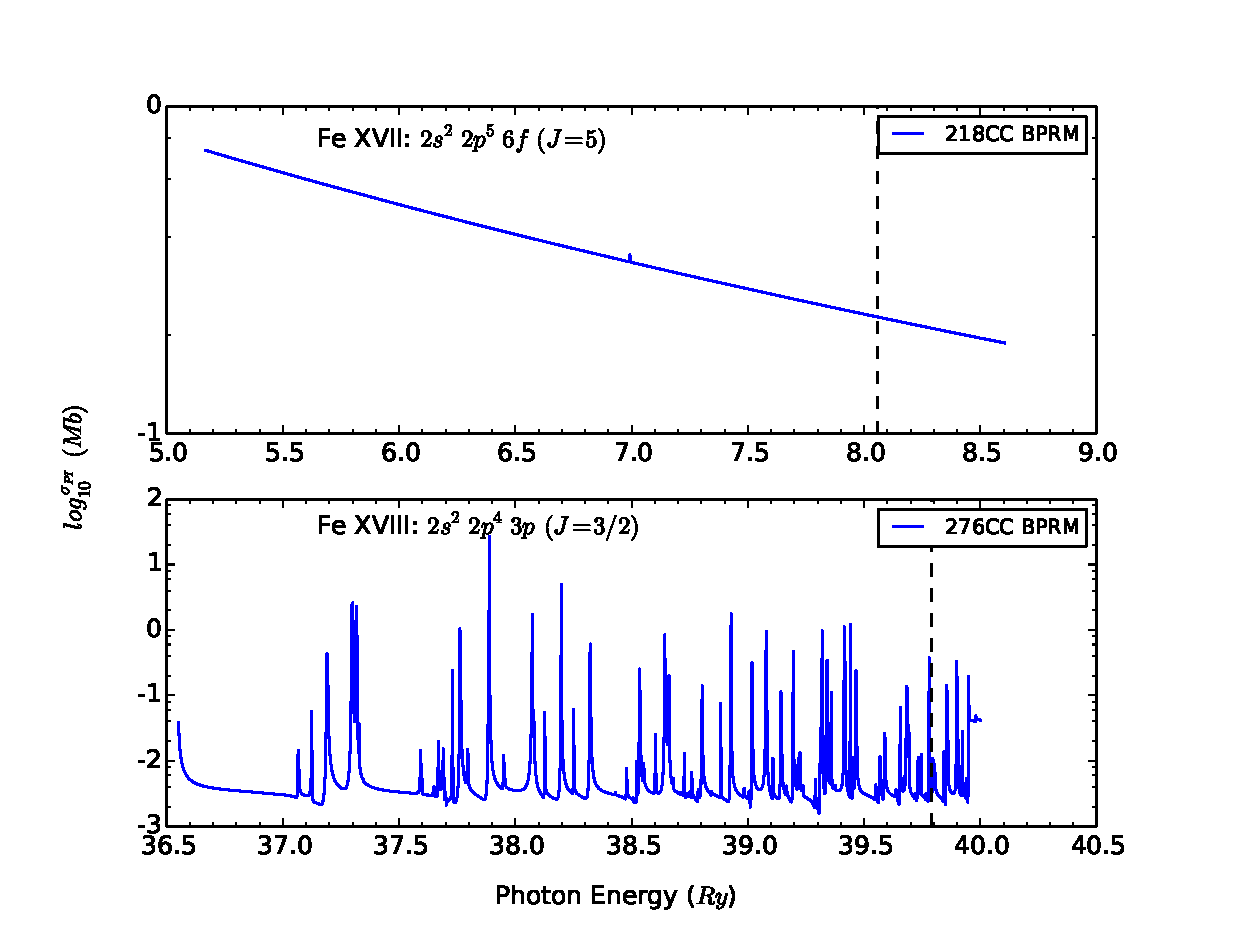
\includegraphics[width=.9\textwidth]{figures_chap_4/negative_region}	
	\caption{The averaged photoionization cross section below the lowest threshold. Dashed vertical line indicates the lowest threshold position.}
	\label{figure_negative_region}
\end{figure}

\subsection{The Ground State of Fe XVII}
The 99LS-RM calculation is done by \citet{99cc_2016}, and the ground state is singlet, i.e. no fine structure, thus this level is not splitted and should match with the one in 218 CC-BPRM calculation. In figure \ref{figure_bound_99_218}, we may easily find that below the lowest threshold, there are many resonances for 218CC-BPRM calculation, but no resonances in 99LS-RM. Though the energy mesh in 218CC-BPRM calculation is about as 10 times dense as the one used in 99LS-RM, there is still a chance that 99LS-RM does not give resonances in this region. Above the lowest threshold, the two results agree very well, but at the tail of 99LS-RM calculation, there are oscillations, which might be due to the insufficient number of continuum basis functions used (see Section \ref{sec_nrang2_oscillation}). 

%======= FIGURE: negative region
\begin{figure}
	\centering
	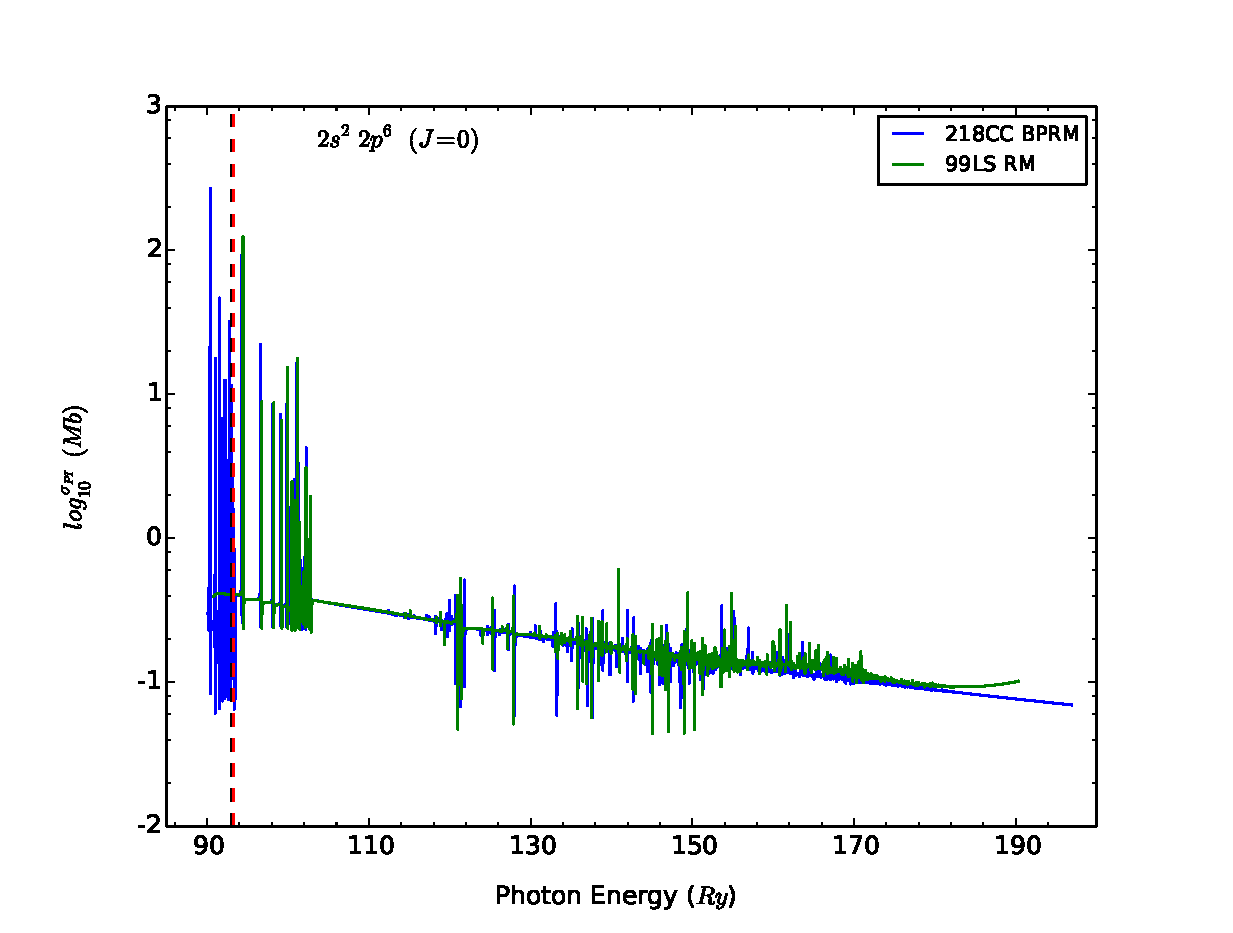
\includegraphics[width=.9\textwidth]{figures_chap_4/fe17_ground_99_218}	
	\caption{The ground state of \ion{Fe}{xvii} in 99LZ-RM and 218 CC-BPRM. The dashed line is the lowest threshold. Black: 218CC-BPRM; red: 99LS-RM. }
	\label{figure_bound_99_218}
\end{figure}


\subsection{MAXC/NRANG2 and Oscillation} \label{sec_nrang2_oscillation}
In the current calculation, the number of continuum basis functions used is 20, which turns out to be insufficient, as it causes oscillations in the photoionization cross section, especially for the high-symmetry bound states (see figure \ref{figure_oscillation}). In figure \ref{figure_oscillation}, we can see that this oscillation happens not only in the high energy region, but also in the lower part, maybe in the middle too. We remove the tail of such oscillations for all states in our opacity calculation (see Chapter \ref{chap_topup}). To overcome this, we may need to increase the number of continuum basis functions, however, this will cause the Hamiltonian matrix size to increase exponentially, thus making the computation extremely hard.
%======= FIGURE: oscillation
\begin{figure}
	\centering
	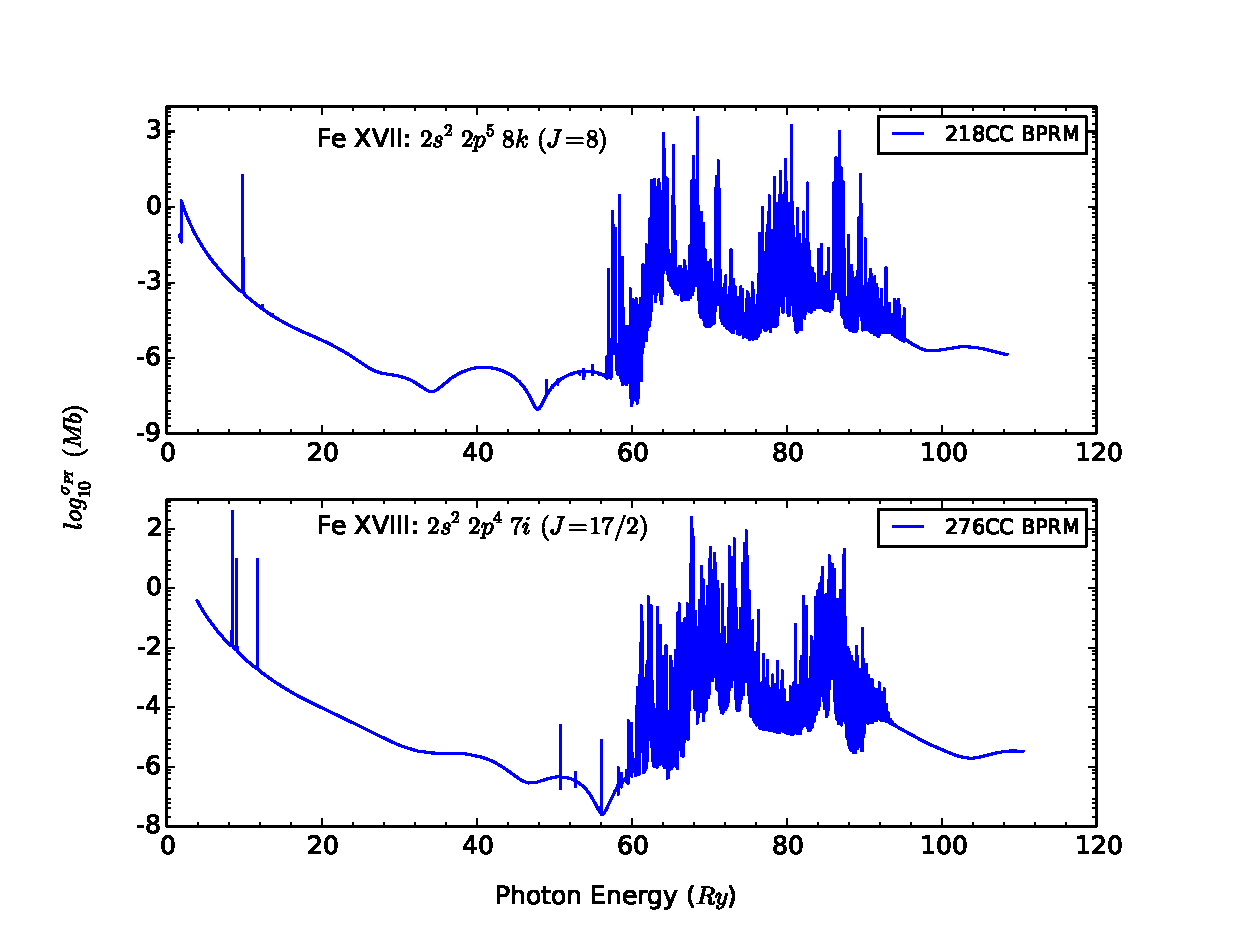
\includegraphics[width=.9\textwidth]{figures_chap_4/oscillation}	
	\caption{The severe oscillations in the photoionization cross section due to small number of continuum basis functions.}
	\label{figure_oscillation}
\end{figure}

\subsection{Resonances}
One of the most salient features of the close coupling approximation is the autoionization resonances due to the coupling between open and closed channels. In the left part of figure \ref{figure_resonance_theory} it  shows a few possible energy levels formed by the core $N$-electron system, and in the right part of the figure, it shows schematically some of the bound levels fomed by coupling each state of the core with an outer electron and these levels just lie below each corresponding core state level. Since we define the ground state of the core having energy of 0, all the bound levels below 0 are purely bound levels, while the levels above are quasi-bound levels. So in BPRM calculation, bound-bound transitions are denoted by A only below 0 energy. While bound-free transitions are between levels below 0 energy line and the ones above 0. There are two kinds of bound-free atomic processes. One is direct photoionization described by open channels, which means the electron is directly photoionized, and the final state is not on the quasi-bound lines. The other is photo-excitation followed by autoionization described by closed channels, and the intermediate state on one of these quasi-bound lines, e.g. a, which can be formed by core state i or other higher core states. Since level a is quasi-bound state, core i can undergo a transition to a lower level, e.g. f1 or f2, without radiation. According to the conservation of energy, the (N+1)th electron now has a positive energy relative to f1 or f2, thus ionized and free. In the following we outline the procedures used to incorporate the resonances.

%======= FIGURE: resonance theory
\begin{figure}
	\centering
	\includegraphics[width=.9\textwidth]{figures_chap_4/resonances_theory}	
	\caption{A diagram showing the bound-bound transitions (A), direct photionization process (B) and photo-excitation-autoionization process (C) treated in BPRM calculation.}
	\label{figure_resonance_theory}
\end{figure}

Define the projection operators $P$ and $Q$ where $P$ projects onto the subspace spanned by the open channels and $Q$ onto the orthogonal subspace, then the Schr\"odinger equation \ref{eq_schodinger} can be rewritten as
\begin{align}
	P(H-E)(P+Q) \Psi_a = 0 \\
	Q(H-E)(P+Q) \Psi_a = 0
\end{align}
, which may be combined into
\begin{equation} \label{eq_resonances}
	P\Bigg(H-PHQ\frac{1}{Q(H-E)Q}QHP-E\Bigg)P\Psi_a = 0
\end{equation}
Define the eigenfunctions of $QHQ$ as 
\begin{equation}
	QHQ\zeta_j = \varepsilon_j\zeta_j
\end{equation}
The second term in equation \ref{eq_resonances} is the optical potential and corresponds to the scattered electron propogating in the orthogonal space $Q$ and it can be expressed as
\begin{equation}
	V_{opt} = \sum_{j=1,m}|PHQ\zeta_j\rangle\frac{1}{\varepsilon_j-E}\langle\zeta_jQHP|
\end{equation}
, so the resonances are due to the poles in $V_{opt}$. 
In the close coupling approximation, the resonances can be due to the closed channels in the expansion \ref{eq_full_expand}. In this case, we can write
\begin{align}
	P\psi_k(x_1\cdot\cdot\cdot x_{N+1}) &= \mathcal{A}\sum_{i}^{NO}\overline{\Phi}_i(x_1\cdot\cdot\cdot x_{N}; \hat{\textbf{r}}_{N+1}\sigma_{N+1}) \frac{1}{r_{N+1}} F_{ik}(r_{N+1}) \\
	Q\psi_k(x_1\cdot\cdot\cdot x_{N+1}) &= \mathcal{A}\sum_{NO+1}^{n}\overline{\Phi}_i(x_1\cdot\cdot\cdot x_{N}; \hat{\textbf{r}}_{N+1}\sigma_{N+1}) \frac{1}{r_{N+1}} F_{ik}(r_{N+1})
\end{align}
, or it can be due to the short-range correlation terms, so in this case, we can write
\begin{align}
	P\psi_k(x_1\cdot\cdot\cdot x_{N+1}) &= \mathcal{A}\sum_{i}^{NO}\overline{\Phi}_i(x_1\cdot\cdot\cdot x_{N}; \hat{\textbf{r}}_{N+1}\sigma_{N+1}) \frac{1}{r_{N+1}} F_{ik}(r_{N+1}) \\
	Q\psi_k(x_1\cdot\cdot\cdot x_{N+1}) &= \sum_{j=1}^m d_{jk} \chi_j(x_1\cdots x_{N+1}) 
\end{align}
In some cases this may cause pseudo-resonances due to inappropriate choose of correlation configurations \citep{pseudo_reso_1, pseudo_reso_2}.

%======= FIGURE: resonances
\begin{figure}
	\centering
	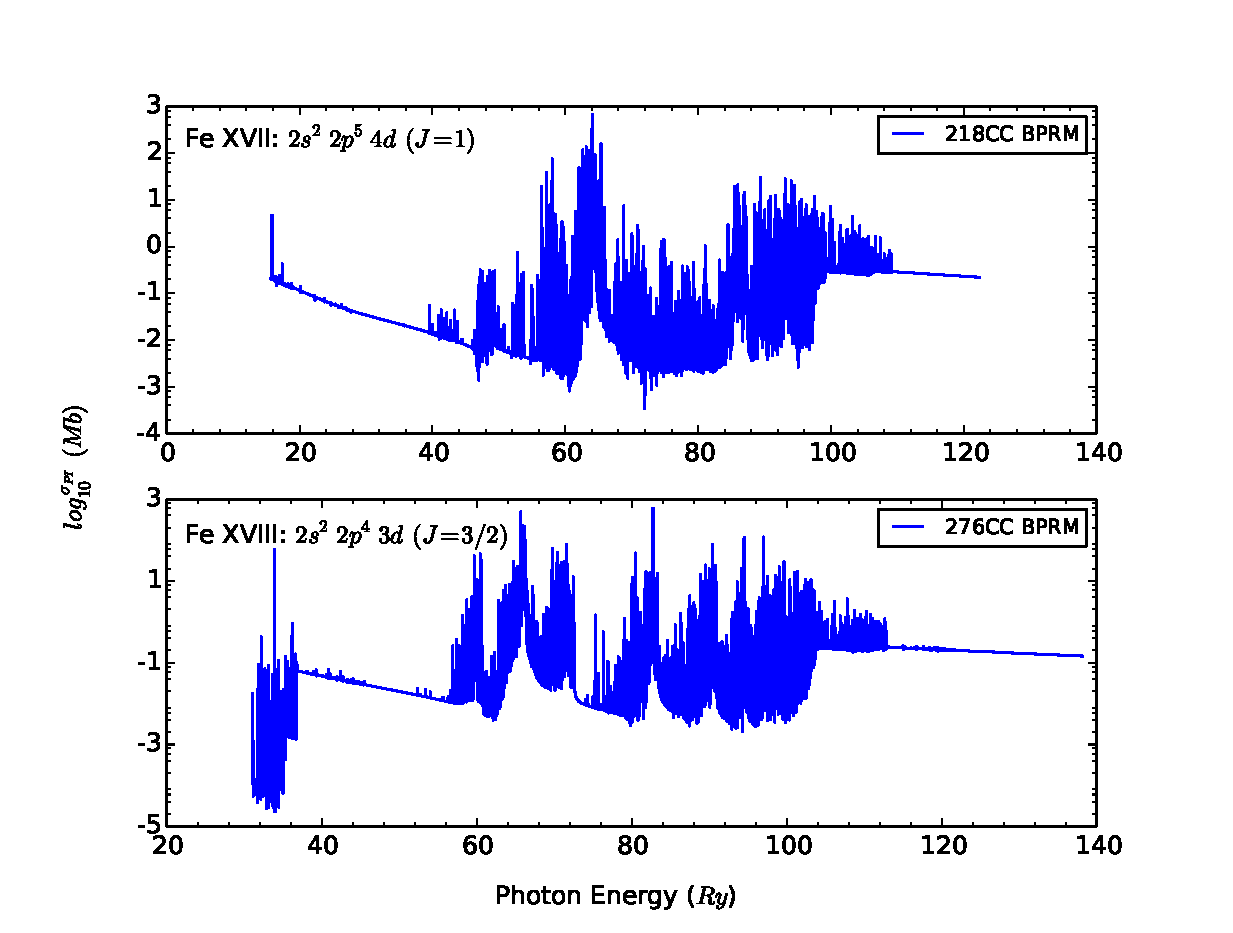
\includegraphics[width=.9\textwidth]{figures_chap_4/resonances}	
	\caption{Rydbeg resonances and PEC.}
	\label{figure_resonances}
\end{figure}

Among the narrow Rydberg resonances, there are considerably broader resonances with greater magnitude, which are called PEC resonances. They are mainly due to the photoexcitation of the core (PEC), where the excitation only occurs in the target leaving the outer electron as a spectator, and these transitions are strong dipole-allowed, i.e. wavefunctions have a considerable radial overlap which was very well studied in \citet{opcd_4} and \citet{pec_2}. In figure \ref{figure_resonances}, we can observe such resonances with very wide width and large magnitude, which modify the photoionization cross section considerably.

\section{Conclusion}
In this chapter, we outlined the formulae used to calculate the radiative data, i.e. oscillator strength and photoionization cross section. we provided the key parameters used in the current BPRM calculations, and gave a brief study on the photoionization cross section just the lowest threshold, the comparison of the ground state of \ion{Fe}{xvii} for 99LS-RM and 218CC-BPRM calculations, the effects of NRANG2 on the data and also the standard Rydberg resonances and PEC resonances. We believe the current calculation gives more accurate atomic data, though improvements can be made on the larger number of continuum basis functions to eliminate the oscillations in the lower energy region.




\chapter{PEC-L-Edge}
\label{chap_pec_l_edge}

\section{Introduction}

The iron opacity at conditions similar to the solar radiation/convection zone boundary was measured at the Sandia National Laboratory \citep{sandia_2015}, revealing wavelength-dependent opacity of 30--400\% higher than the predictions by theoretical opacity models.
To resolve this discrepancy, extensive close-coupling Breit--Pauli $R$-Matrix (BPRM) calculations have been carried out for \ion{Fe}{xvii} including 60 fine-structure levels within the $n\leq 3$ complexes in the \ion{Fe}{xviii} target ion \citep[60CC-BPRM,][]{60cc_2011} and 99 $LS$ terms within $n\leq 4$ (99LS-RM). They show strong photon absorption due to core excitation, resulting in an increment of 35\% in the Rosseland mean opacity over the Opacity Project (OP) data \citep [][hereafter NP16]{99cc_2016}. The convergence of photoionization cross section demonstrated in NP16 is criticized by \citet{more_comment_2017}, pointing out the underestimated photon absorption for levels with the outer electron of $n~>~4$. Such criticism is addressed in the current study. 

In section \ref{section_pec_l_edge}, the transition type that causes the jump of the background of the photoionization cross section in NP16 is identified. Such transitions occur around the same photon energy for each ion, and it turns out they are $99~Ry$, $106~Ry$ and $114~Ry$ for \ion{Fe}{xvii}, \ion{Fe}{xviii} and \ion{Fe}{xix}, respectively. The photoionization cross section due to these transitions is orders-of-magnitude larger than the other types of L-edge bound-free tansitions. To distinguish it from other types of L-edge transitions, we name it as PEC-L-Edge transition. In the same section, a systematic study is given for PEC-L-Edge transitions.


\section{PEC-L-Edge}
\label{section_pec_l_edge}
To identify the type of transitions that cause the jump of the background of photoionization cross section in BPRM calculation, we use FAC package \citep{gu_2008} to carry out the photoionization cross section including the same core configurations as those included in BPRM calculation, and match the bound levels by comparing the total angular momentum, parity, energy and photoionization cross section (see Section \ref{section_matching} for more details), and finally pick the transitions that contribute the most of photoionization cross section. In FAC, it outputs a table that lists all transitions, each of which is computed at six widespread points by default, and we consider the photoionization cross section at the first default point in the order of $0.01~Mb$ as large. In the rest of this section I will give a few examples of PEC-L-Edge transitions, followed by a systematic study of their ionization thresholds and photoionization cross section for \ion{Fe}{xvii}, \ion{Fe}{xviii} and \ion{Fe}{xix}.

\subsection{PEC-L-Edge in BPRM and RDW}
To give a clear illustration of PEC-L-Edge transitions, we take the ground state of \ion{Fe}{xvii} as an example (see figure \ref{fig_fe17_ground}). In the current BPRM (see Chapter \ref{chap_bprm_fe17_fe18}) calculation for \ion{Fe}{xvii}, the core configurations included are ${2s^2 2p^5}$, ${2s 2p^6}$, ${2s^2 2p^4 n\ell}$, ${2s 2p^5 n\ell}$, ${2p^6 3\ell'}$, where $n=3, ~4$, and $\ell,~ \ell'\leq2$, which result in 218 fine structure levels of the core. In the RDW calculation, the same core configurations are included. After extracting the transitions that give the large photoionization cross section, we find the final ionized states are the three levels in ${2s^2 2p^5}$ and ${2s 2p^6}$, and their ionization thresholds are $92.3~Ry$, $93.2~Ry$ and $102.3~Ry$. Though there are no electrons outside of L-shell, we can still treat one $2p$ electron as the outer electron, and the rest $2s,~2p$ electrons belong to the core. Thus PEC-L-Edge transitions happen when only one $2s$ or $2p$ electron is ionized, keeping the other electrons unchanged. In figure \ref{fig_fe17_ground}, the three PEC-L-Edge transitions successfully reproduce the background of BPRM calculation. Though there are many transitions above $150~Ry$, they are negligibly small when compared with the PEC-L-Edge transitions.

%======Figure Fe17_ground
\begin{figure}
	\centering
	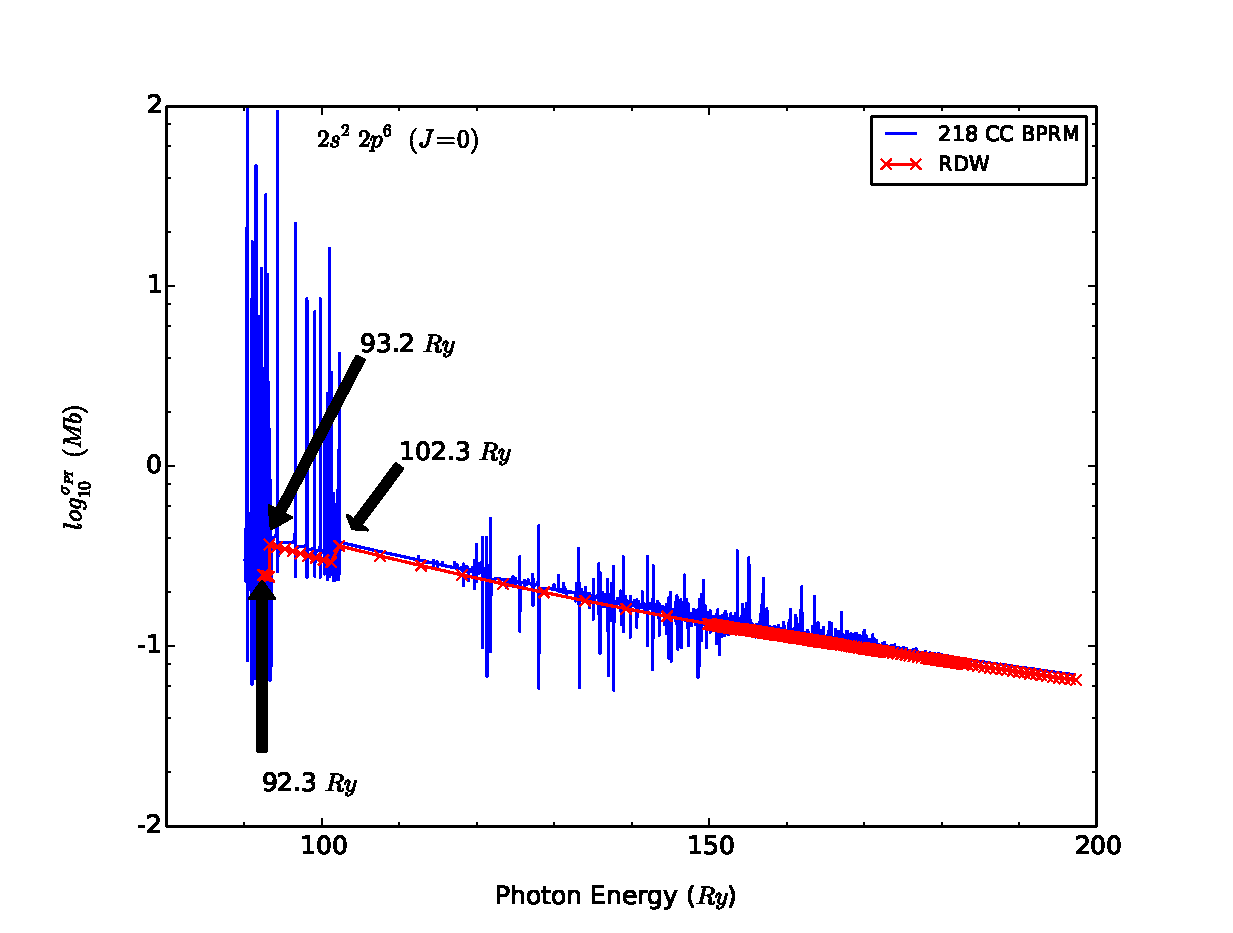
\includegraphics[width=\textwidth]{figures_5/fe17_ground.eps}	
	\caption{The photoionization of the ground state of \ion{Fe}{xvii}. The three PEC-L-Edge transitions using FAC reproduce the background of the photoionization cross section in BPRM calculation. The thresholds of these PEC-L-Edge transitions are marked. The energy mesh is created such that 10 points are uniformly distributed between adjacent thresholds.}
	\label{fig_fe17_ground}
\end{figure}

In the current \ion{Fe}{xviii} BPRM calculation (see Chapter \ref{chap_bprm_fe17_fe18}), the core configurations included are $2s^2 2p^4$, $2s 2p^5$, $2p^6$, $2s^2 2p^3 3\ell$, $2s 2p^4 3\ell$, $2s^2 2p^3 4\ell$, where $\ell\leq2$, which yield 276 fine structure levels of the core. Since the core configurations of $n=3$ and $n=4$ are not completely included, some bound levlels with the outer electron in M- or N-shell will not get the full contribution from PEC-L-Edge transitions. For example, for level $2s^22p^44d~(J=5/2)$ in figure \ref{fig_fe18_5_0_20}, the top panel shows excellent reproduction of the background by RDW, showing various steps before coming to a big jump, though the energies are off a tiny bit. By extracting the main transitions in FAC, we find the jump is due to the PEC-L-Edge transitions to levels in $2s^2 2p^3 4d$. When doing the top up calculation for this level (see Section \ref{section_other_targets}), we extend the BPRM data to higher energy region using RDW data (the dash-dotted line in the bottom panel), which is mainly due to the PEC-L-Edge transitions to levels in $2s^2 2p^3 4d$, and add the contribution from other unincluded core configurations up to $n=10$ (the black line in the bottom panel), which is mainly due to the PEC-L-Edge transitions to levels in $2s 2p^4 4d$. 

In the current \ion{Fe}{vii} and \ion{Fe}{xviii} BPRM calculation, all such jumps are reproduced by RDW calculation (see \url{https://github.com/zhao1157/PhD-Atomic-Physics/tree/master/fe17\_fe18\_matched\_levels}), and we believe the type of transitions that cause such jump of background is identified, i.e. PEC-L-Edge transition, which falls in the spectator-electron process category \citep{mendoza_2018}. In \citet{mendoza_2018}, the study case on the K-edge of \ion{O}{vi} can be explained in the similar way like PEC-L-Edge in our study. As for the high-n levels that do not show such PEC-L-Edges, the top up calculation complements such missing jumps (see figure \ref{fig_fe17_fe18_other_jump}). In both  \ion{Fe}{vii} and \ion{Fe}{xviii} BPRM calculations, the core configurations included do not have $n>4$, so the bound levels with outer electron of $n=5,~7$ do not have PEC-L-Edges in BPRM calculation. In the top up calculation, we consider all bound levels with $n\leq10$, so we include the core configurations with $n\leq10$ in order to obtain the PEC-L-Edge for each level.

In NP16, the convergence of the photoionization cross section is demonstrated by showing two levels which have such PEC-L-Edge background that dominates most of the resonances in the higher energy region, however, there are many other levels that do not have such PEC-L-Edge background, for example figure 4(b) in NP16, which is correctly pointed out by \citet{more_comment_2017} that it is due to missing $n>4$ core configurations, thus it is not sufficient to prove the convergence of the photoionization cross section by considering only two levels. And the enhancement obtained by 99LS-RM over 60CC-BPRM (or 30CC as referred to in NP16) calculation for the two levels shown in figure 3(b, c) in NP16 is due to the core configurations $2s2p^53p$ and $2s2p^53d$, which are not included in 60CC-BPRM, but in 99LS-RM. In the current BPRM calculation complemented by RDW calculation, all bound levels have such PEC-L-Edge backgound starting around $100~Ry$, thus the photoionization cross section is converged. In the rest of this section, I will show two properties that are very important to PEC-L-Edge transitions.

%======Figure fe18_5_0_20
\begin{figure}
	\centering
	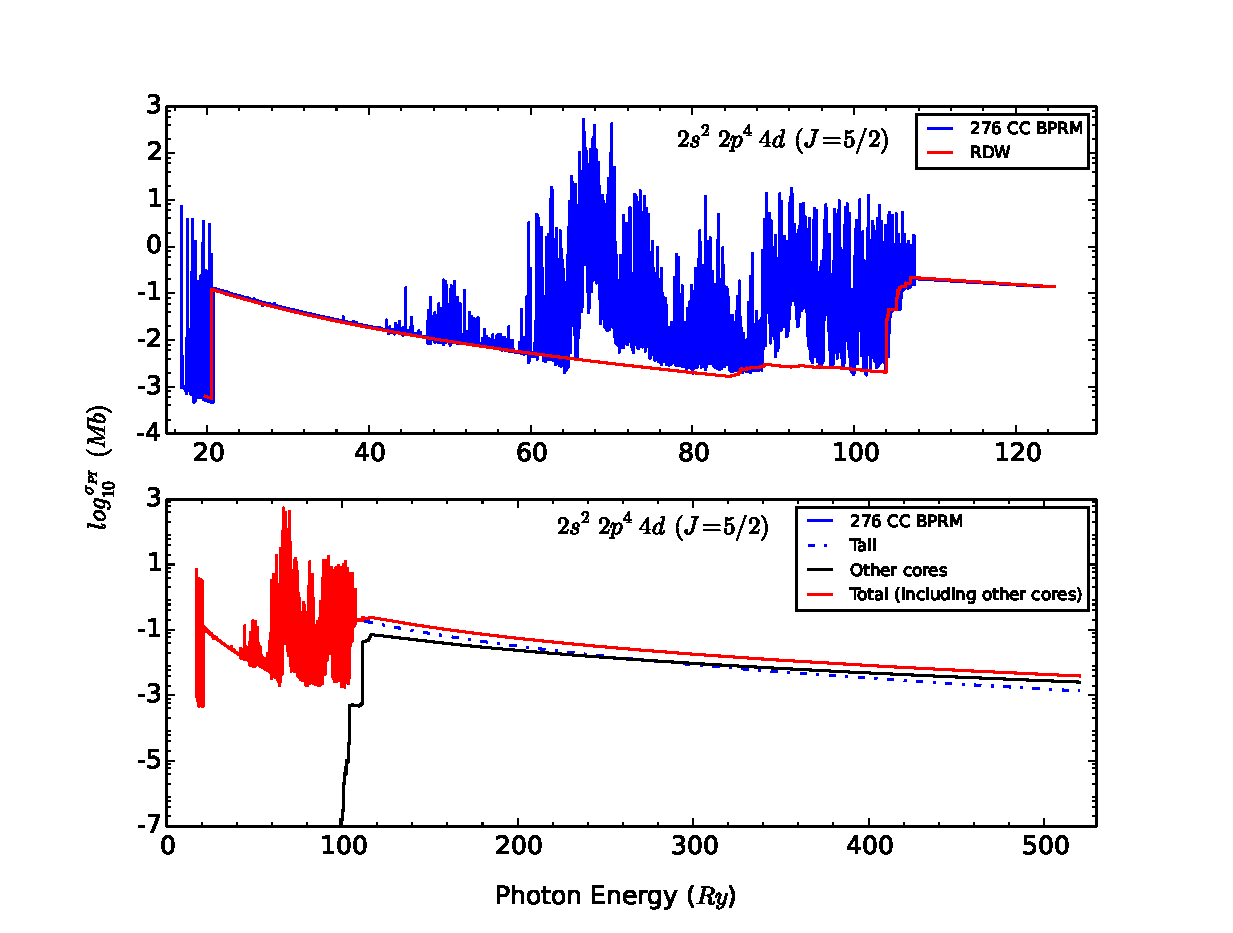
\includegraphics[width=\textwidth]{figures_5/fe18_5_0_20}	
	\caption{The photoionization cross section of level $2s^22p^44d~(J=5/2)$ in \ion{Fe}{xviii}. In the top panel, RDW calculation reproduces the background of BPRM calculation; in the bottom panel, the BPRM calculation is extended with a tail in higher energy region (blue dash-dotted line) using RDW and the contribution from other core configurations up to $n=10$ (black line) is added, giving the total photoionization cross section (red line).}
	\label{fig_fe18_5_0_20}
\end{figure}

%======Figure fe17_fe18_other_jump
\begin{figure}
	\centering
	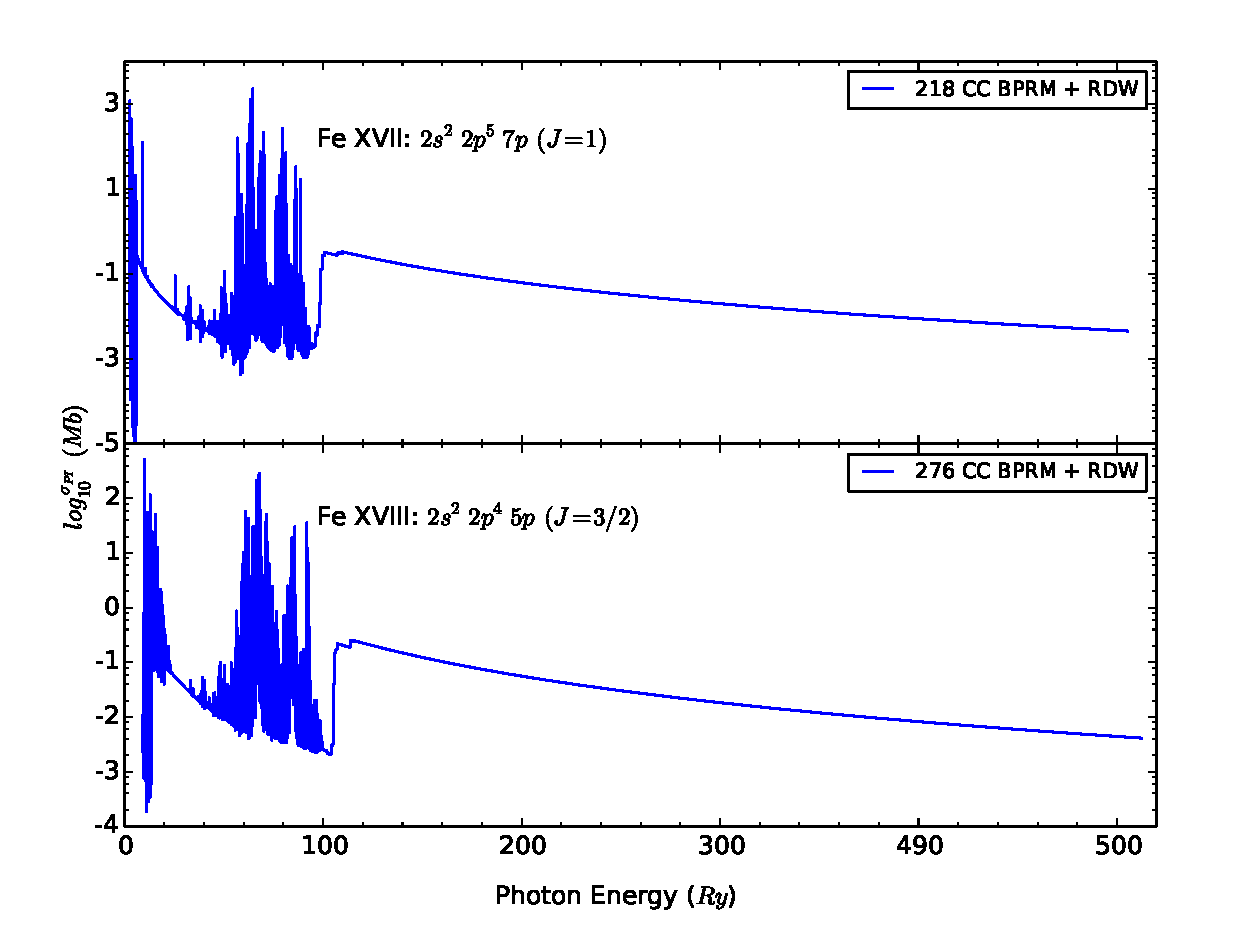
\includegraphics[width=\textwidth]{figures_5/fe17_fe18_other_jumps}	
	\caption{The photoionization cross section of level $2s^22p^57p~(J=1)$ in \ion{Fe}{xvii} and level $2s^22p^45p~(J=3/2)$ in \ion{Fe}{xviii}. The PEC-L-Edge shows up in both levels when high-n core configurations are included in the top up calculation.}
	\label{fig_fe17_fe18_other_jump}
\end{figure}

\subsection{Properties of PEC-L-Edge}
\label{section_propertie_pec_l_edge}
Pure RDW calculations are carried out for \ion{Fe}{xvii}, \ion{Fe}{xviii} and \ion{Fe}{xix} to study the properties of these PEC-L-Edge transitions, and we find for each ion, the PEC-L-Edge background starts around the same photon energy, i.e. $100~Ry$, $106~Ry$ and $114~Ry$ for  \ion{Fe}{xvii},  \ion{Fe}{xviii} and \ion{Fe}{xix}, respectively. And the photoionization cross section is large and varies little from level to level.

To demonstrate the PEC-L-Edge transitions occurring around the same photon energy, see diagram \ref{fig_fe17_fe18_fe19_thresholds}. Since the PEC-L-Edge transitions only ionize one electron from $2s$ or $2p$ subshell, while keeping ther other electrons as spectators, the ionization threshold is 
\begin{align}
\label{equ_ionization}
\Delta E (Ry)&= \Delta I - \frac{(z+1)^2}{n^2} + \frac{z^2}{n^2} \nonumber  \\
 			   &= \Delta I - \frac{1+2z}{n^2}.
\end{align}
For \ion{Fe}{xvii}, \ion{Fe}{xviii} and \ion{Fe}{xix}, $z = 17,~18,~19$, respectievly, and $n$ takes intergers from 2 to 10, thus the second term in equation \ref{equ_ionization} is approximately less than $1~Ry$ when $n\geq6$ and this proves the ionization thresholds being around the same value for each ion. When $n=2$, the second term gives a difference of $8.75~Ry$, $9.25~Ry$ and $9.75~Ry$ for  \ion{Fe}{xvii}, \ion{Fe}{xviii} and \ion{Fe}{xix}, respectively.

%======Figure ionization_threshold
\begin{figure}
	\centering
	\includegraphics[width=.9\textwidth]{figures_5/ionization_energy}	
	\caption{The diagram of ionization threshold of PEC-L-Edge transitions. PEC-L-Edge transitions only happen between initial level in configuration $2\ell^x~n\ell'$ and final level in $2\ell^{x-1}~n\ell'$, and the ionization threshold is denoted by $\Delta E$. $\Delta I$ is the energy difference between core configurations $2l^x$ and $2l^{x-1}$, and the energy of level $2\ell^x~n\ell'$ is $\frac{z^2}{n^2}$ below the core  $2l^x$, and the energy of level $2\ell^{x-1}~n\ell'$ is $\frac{(z+1)^2}{n^2}$ below the core  $2l^{x-1}$.}
	\label{fig_fe17_fe18_fe19_thresholds}
\end{figure}

%======Figure ionization_threshold_start_end
\begin{figure}
	\centering
	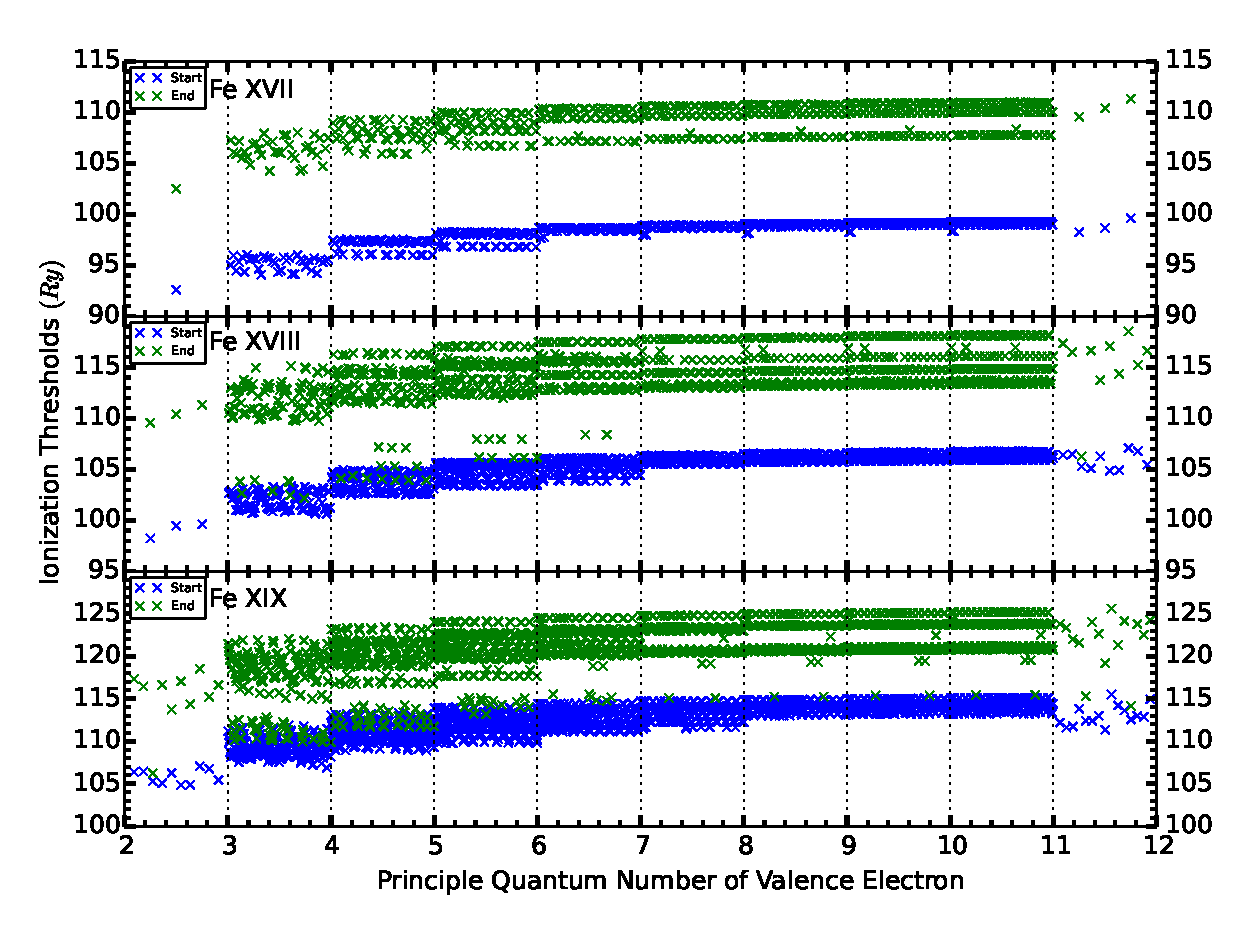
\includegraphics[width=\textwidth]{figures_5/fe17_fe18_start_end}	
	\caption{The thresholds of PEC-L-Edge transitions for  \ion{Fe}{xvii}, \ion{Fe}{xviii} and \ion{Fe}{xix} in pure RDW calculation. Blue ``$\times$'' refers to the lowest (starting) threshold of PEC-L-Edge transition and green ``$\times$'' the highest (ending) threshold of PEC-L-Edge transition. In region 11-12, these data points are for the core configurations without the outer electron.}
	\label{fig_fe17_fe18_fe19_thresholds_start_end}
\end{figure}

%======Figure fe17_fe18_fe19_end_500_PI
\begin{figure}
	\centering
	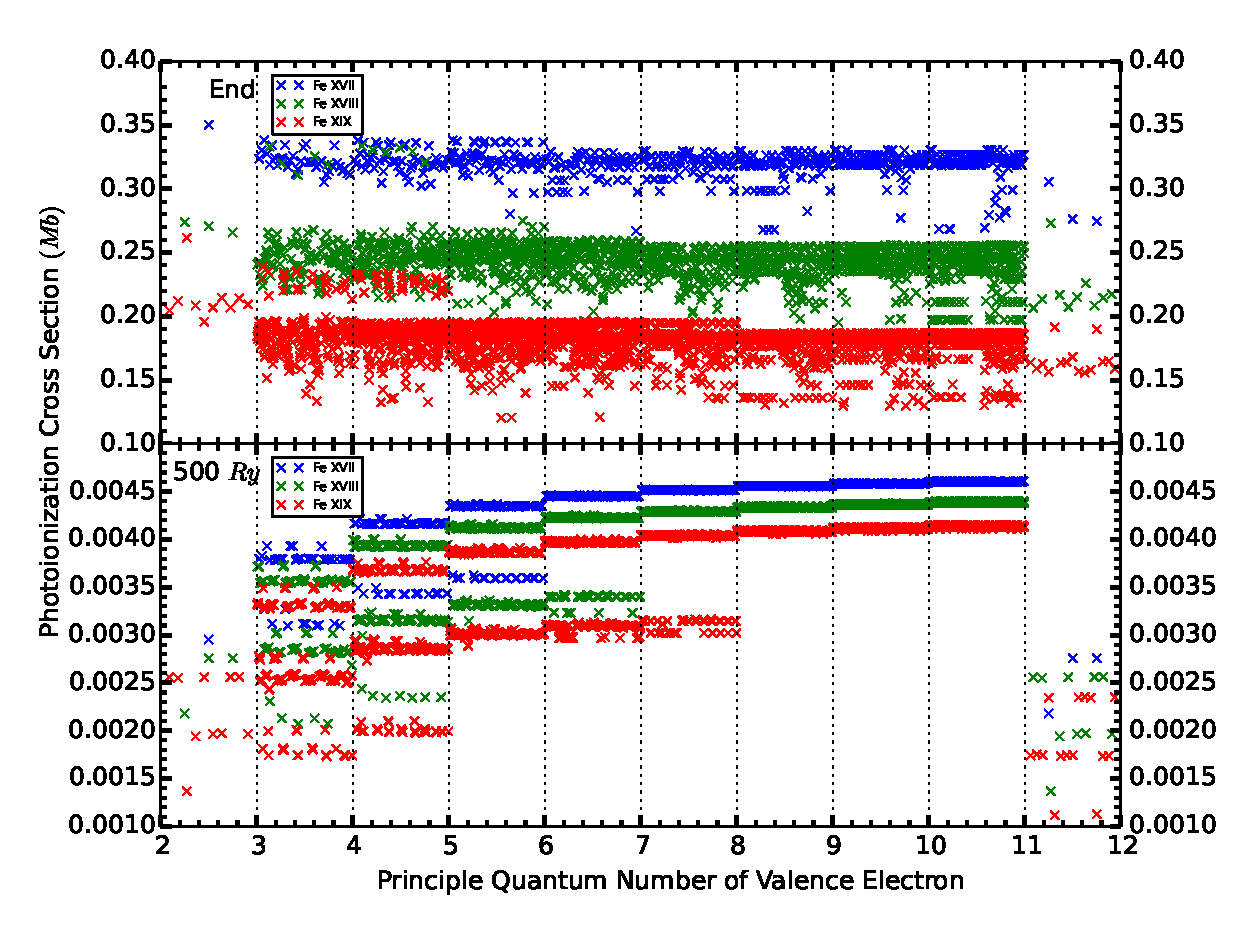
\includegraphics[width=\textwidth]{figures_5/fe17_fe18_end_500}	
	\caption{The photoionization cross section of PEC-L-Edge transitions for  \ion{Fe}{xvii}, \ion{Fe}{xviii} and \ion{Fe}{xix} at energies just above the thresholds denoted by``End'' in figure \ref{fig_fe17_fe18_fe19_thresholds_start_end} and at $500~Ry$. In region 11-12, these data points are for the core configurations without the outer electron and the photoionization cross section in the top panel is the maximum value above the lowest PEC-L-Edge threshold.}
	\label{fig_fe17_fe18_fe19_pi_end_500ry}
\end{figure}

In the pure RDW calculation, we consider all bound levels with the principle quantum number of the outer electron within 10, so in order to get PEC-L-Edge background for each level, the core configurations with $n\leq10$ are included and only same-n-complex configuration interaction for bound and core configurations is considered. The number of bound levels for  \ion{Fe}{xvii}, \ion{Fe}{xviii} and \ion{Fe}{xix} is 587, 1590 and 2613, respectively. In figure \ref{fig_fe17_fe18_fe19_thresholds_start_end}, the lowest threshold (blue ``$\times$'') of PEC-L-Edge transition is plotted against the principle quantum number of the outer electron. For all levels with the same quantum number $n$ of the outer electron, they are uniformly distributed in region ($n,~n+1$). In region (11, 12), these points are for the core configurations with the outer electron removed. Just as equation \ref{equ_ionization} predicts, the PEC-L-Edge transitions start around the same energy for $m\geq6$, and $\Delta I$ is $99~Ry$, $106~Ry$ and $114~Ry$ for \ion{Fe}{xvii}, \ion{Fe}{xviii} and \ion{Fe}{xix}, respectively, which approaches the ionization thresholds of the core without the outer electron, as shown in region (11, 12). For low-n bound levels, for example $n=2$, the lowest ionization threshold is $93~Ry$, $98~Ry$ and $105~Ry$ for \ion{Fe}{xvii}, \ion{Fe}{xviii} and \ion{Fe}{xix}, respectively, which falls around the region predicted by equation \ref{equ_ionization}. To study the photoionization cross section due to PEC-L-Edge transitions in higher-energy region, we calculate it at energy just above the highest threshold of PEC-L-Edge transition for each level (denoted by green ``$\times$'' in figure \ref{fig_fe17_fe18_fe19_thresholds_start_end}) and at $500~Ry$ and the result is shown in figure \ref{fig_fe17_fe18_fe19_pi_end_500ry}. For each ion, the photoionization cross section fluctuates in a small region at energies marked as ``End'' and at $500~Ry$, and values in between approximately follow  as \(\sigma(\nu) \propto E^{-3}\). It is almost independent of the outer electron, and it is a little higher than the result of the core configurations with the outer electron removed.




\section{Conclusion}
The type of strong dipole-allowed transitions in L-shell photoionization cross section in BPRM calculation is identified by RDW calculation, i.e. PEC-L-Edge transition type, which ensures the large PEC-L-Edge background for all bound levels that are considered in the current BPRM+RDW calculation (see Chapter \ref{chap_topup}). Two properties of the PEC-L-Edge transitions for \ion{Fe}{xvii}, \ion{Fe}{xviii} and \ion{Fe}{xix} are investigated, one of which is roughly the same starting threshold of PEC-L-Edge transition for high-n levels, i.e. $99~Ry$ for \ion{Fe}{xvii}, $106~Ry$ for \ion{Fe}{xviii} and $114~Ry$ for \ion{Fe}{xix}, and the other is that the PEC-L-Edge background dominates in the high-energy region and is not much affected by the high-n outer electron.



\chapter{Top-Up Calculations for \ion{Fe}{XVII} and \ion{Fe}{XVIII}} \label{chap_topup}

%========1. INTRODUCTION ==========
\section{Introduction}

The iron opacity at conditions similar to the solar radiation/convection zone boundary was measured at the Sandia National Laboratory \citep{sandia_2015}, revealing wavelength-dependent opacity of 30--400\% higher than the predictions by theoretical opacity models.
To resolve this discrepancy, extensive close-coupling Breit--Pauli $R$-Matrix (BPRM) calculations have been carried out for \ion{Fe}{xvii} including 60 fine-structure levels within the $n\leq 3$ complexes in the \ion{Fe}{xviii} target ion \citep[60CC-BPRM,][]{60cc_2011} and 99 $LS$ terms within $n\leq 4$ (99LS-RM). They show strong photon absorption due to core excitation, resulting in an increment of 35\% in the Rosseland mean opacity over the Opacity Project (OP) data \citep [][hereafter NP16]{99cc_2016}. Whereas the NP16 work demonstrated that in the $R$-Matrix opacity calculations convergence of the close-coupling expansion was a necessary condition for accuracy, completeness of all possible excited configurations at Z-plasma temperatures still requires additional contributions in the high-energy region \citep{comment_2016, comment_2016a, more_comment_2017}.

At Z-plasma condition,  \ion {Fe}{xvii}, \ion{Fe}{xviii} and \ion{Fe}{xix} are the three dominant iron ions with ionization fractions of 0.19, 0.38 and 0.29, respectively \citep{99cc_2016}. And in this paper, we adopt the 218CC-BPRM calculation for \ion{Fe}{xvii} and 276CC-BPRM calculation for \ion{Fe}{xviii} \citep{rmop_2}, and top-up the bound-bound and bound-free data with relativistic distorted wave (RDW) data using flexible atomic code (FAC) \citep{gu_2008}.

In the following sections, the specifications of the 218CC- and 276CC-BPRM calculations of \citet{rmop_2} are summarized, followed by the ``top-up'' configurations and transitions calculated using FAC. To ensure data correspondence from FAC, a procedure of matching the bound levels from BPRM and FAC is described. And the bound-bound and bound-free top-up calculation is detailed afterwards. 


%==========2. BPRM ==========
\section{\ion{Fe}{XVII} and \ion{Fe}{XVIII} BPRM} \label{bprm}
Close coupling approximation introduces autoionizing resonances in the photoinization cross section, which may severely suffer from radiative damping for H- or He-like highly charged ions, thus reduce photionization cross section considerably, however, for \ion{Fe}{xvii} and \ion{Fe}{xviii}, such effect is negligible \citep{ah_1997, zhang_1998, hsa_1999}. So undamped photoionization cross section is used in the opacity calculation \citep{rmop_5}. 

The current BPRM calculations for \ion{Fe}{xvii} and \ion{Fe}{xviii} are the largest as far as we know, with the maximum number of free channels of 998 and 1288, respectively \citep{rmop_2}. For \ion{Fe}{xvii}, 99LS-RM calculation \citep{99cc_2016} is extended to 218CC-BPRM by including the fine structure of the target states. The target configurations ($1s$ is always full, so omitted for brevity) included are ${2s^2 2p^5}$, ${2s 2p^6}$, ${2s^2 2p^4 n\ell}$, ${2s 2p^5 n\ell}$, ${2p^6 3\ell'}$, where $n=3, ~4$, and $\ell,~ \ell'\leq2$, which have 99 $LS$ terms, or 218 fine structure levles. The continuum orbitals included are $\ell\leq 9$, and the number of continuum $R$-Matrix basis functions included is 20, and the bound states are found by scanning the effective quantum number within 10.1 \citep{seaton_bound_1985, berrington_seaton_1985}. However, such technique does not provide the spectroscopy notations for the bound levels obtained, nor guarantee that all the bound levels are found within the effective quantum number range of interest. To resolve the first issue, \citet{nahar_levelid_2000} developed such a program that can identify most of the bound levels spectroscopically, and the rest a few highly mixed levels remain undetermined \citep{nahar_fev_2000}, which might be overcome by comparing some physical quantities of these levles caculated by FAC, for example the photoionization cross section to be described in the next section. The second issue depends on the scanning step employed and 0.001 gives fewer bound levels in the 218CC-BPRM than 60CC-BPRM, so a finer step 0.0001 or 0.0005 is used in the region where levels are missing, which finally gives 464 bound levels, which is 10 more than 60CC-BPRM. 

For \ion{Fe}{xviii}, two sets of BPRM calculation are done with different target configurations. One includes up to $n=3$ target configurations, i.e. $2s^2 2p^4$, $2s 2p^5$, $2p^6$, $2s^2 2p^3 3\ell$, $2s 2p^4 3\ell$, where $\ell\leq2$, which yield 200 target fine structure levels. In addition to the above target configurations,  the other BPRM calculation includes $n=4$ configurations, i.e. $2s^2 2p^3 4\ell$, where $\ell\leq2$, which yield 276 fine structure levels. The parameters set for the continuum orbitals and basis functions are the same as \ion{Fe}{xvii}  218CC-BPRM calculation. 200CC-BPRM calculation finds 1149 bound levels with scanning step of 0.001, while 276CC-BPRM calculation finds 1163 bound levels with 0.001 as the first attemp scanning step and 0.0001 or 0.0005 as the second in the region where levels are missing compared with 200CC-BPRM.

In the opacity calculation, the oscillator strength from the 60CC-BPRM and 200CC-BPRM calculations and the photoionization cross section from the 218CC-BPRM and  276CC-BPRM calculations are used \citep{rmop_5}. So in doing the FAC top up calculation, matching the bound levels for each BPRM calculation is necessary in that they have different number of bound levels, and even in some region where levels are so closely packed (see table \ref{packed_levels}), the order of these levels may shuffle (see figure \ref{mismatch}). In figure \ref{fe17_n3_n4_mismatch}, photoionization cross section of 6 levles of \ion{Fe}{xvii} is plotted for 60CC-BPRM and 276CC-BPRM and we find distinct difference in level 24 and 26. Similar issue arises in figure \ref{fe18_n3_n4_mismatch} of \ion{Fe}{xviii}. Even though these levels have similar energy, they may have distinctive configurations (see section \ref{section_matching}), which is the reason why we should redo the identification for different CC-BPRM calculations. Afte being switched, these levels show good agreement (see figure \ref{fe17_n3_n4_rematch} and \ref{fe18_n3_n4_rematch}).

%======== TABLE: closely packed levels ======
\begin{table}
	\centering
	\caption {Selected packed levels of \ion{Fe}{xvii} ($J = 4, \pi = o$) and \ion{Fe}{xviii} ($J=5/2, \pi=o$) (Note: the energy is $z$-scaled, and in unit of $10^{-2} Ry$)}
	\begin{tabular}{|c || c | c | c|}
		\hline
		& level index & 60CC-BPRM & 218CC-BPRM \\
		\hline
		\multirow{6}{*}{\ion{Fe}{xvii}} & 23 & -1.242945 & -1.239702 \\
		& 24 & -1.239540 & -1.238049 \\
		& 25 & -1.237855 & -1.236506 \\
		& 26 & -1.236421 & -1.235733 \\
		& 27 & -1.235081 & -1.235227 \\
		& 28 & -1.234742 & -1.234723 \\
		\hline
		\hline
		& level index & 200CC-BPRM & 276CC-BPRM \\
		\hline
		\multirow{3}{*}{\ion{Fe}{xviii}} & 31 & -3.996445 & -4.004678 \\
		& 32 & -3.993010 & -4.003468 \\
		& 33 & -3.989362 & -4.000058 \\
		\hline
	\end{tabular}	
	\label{packed_levels}
\end{table}

%======= FIGURE: n3 ,n4 mismatch
\begin{figure}
	\centering
	\subfloat[\ion{Fe}{xvii}: before level 24 and 26 being switched]{
		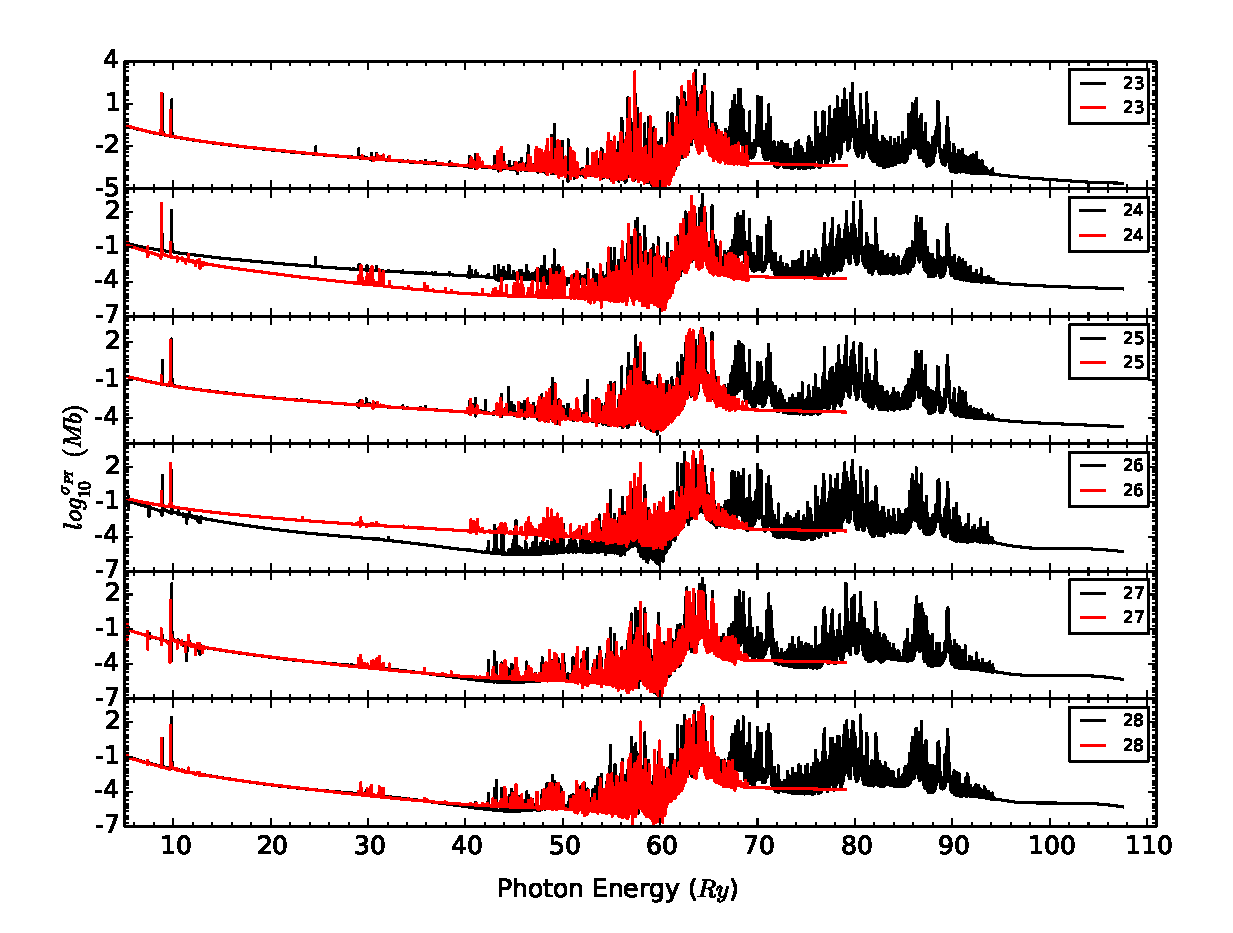
\includegraphics[width=0.49\textwidth]{figures/fe17_n3_n4_mismatch}
		\label{fe17_n3_n4_mismatch}
	}
~
	\subfloat[\ion{Fe}{xviii}: before level 31 and 33 being switched]{
		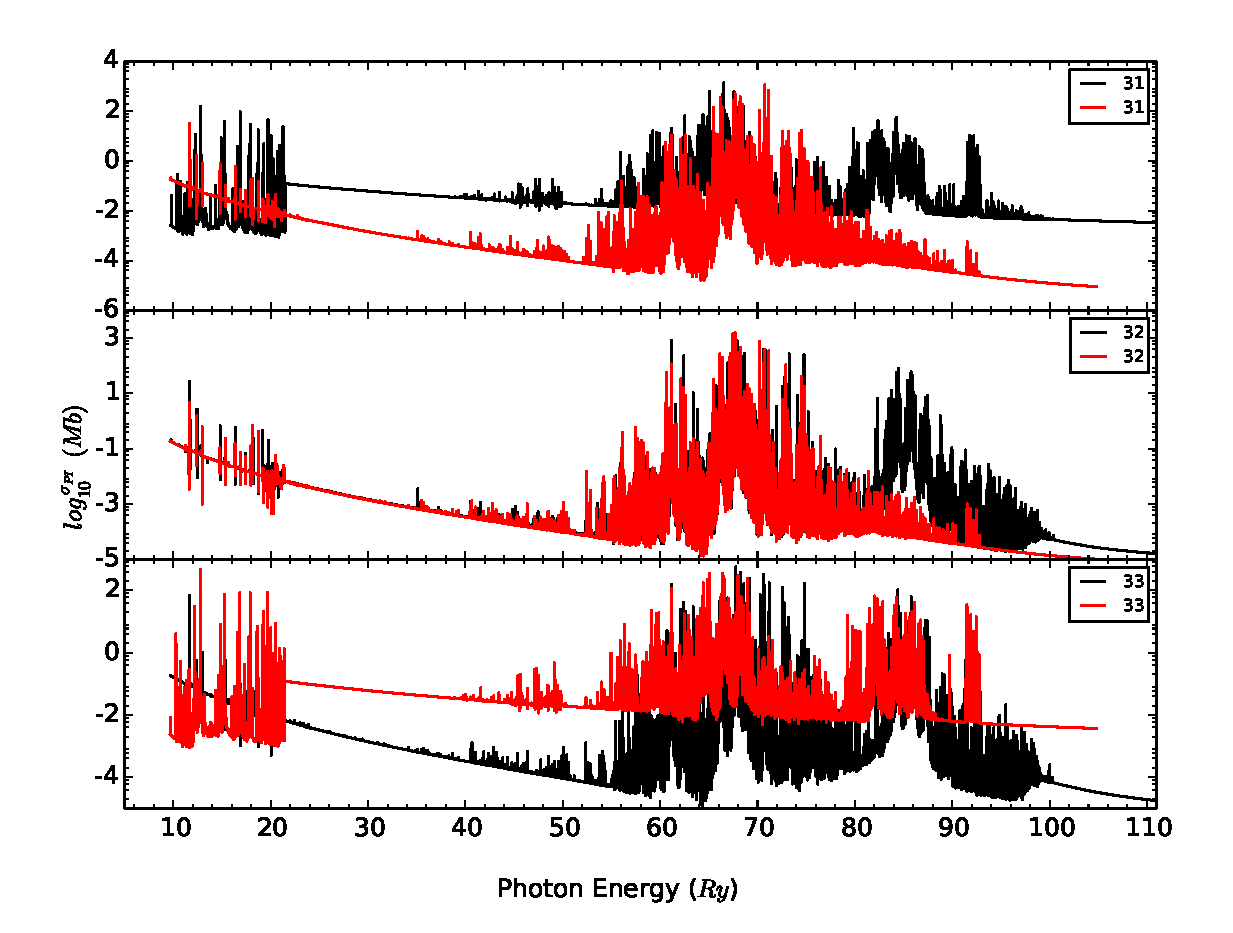
\includegraphics[width=0.49\textwidth]{figures/fe18_n3_n4_mismatch}
		\label{fe18_n3_n4_mismatch}
	}
	
	\subfloat[\ion{Fe}{xvii}: after level 24 and 26 being switched]{
		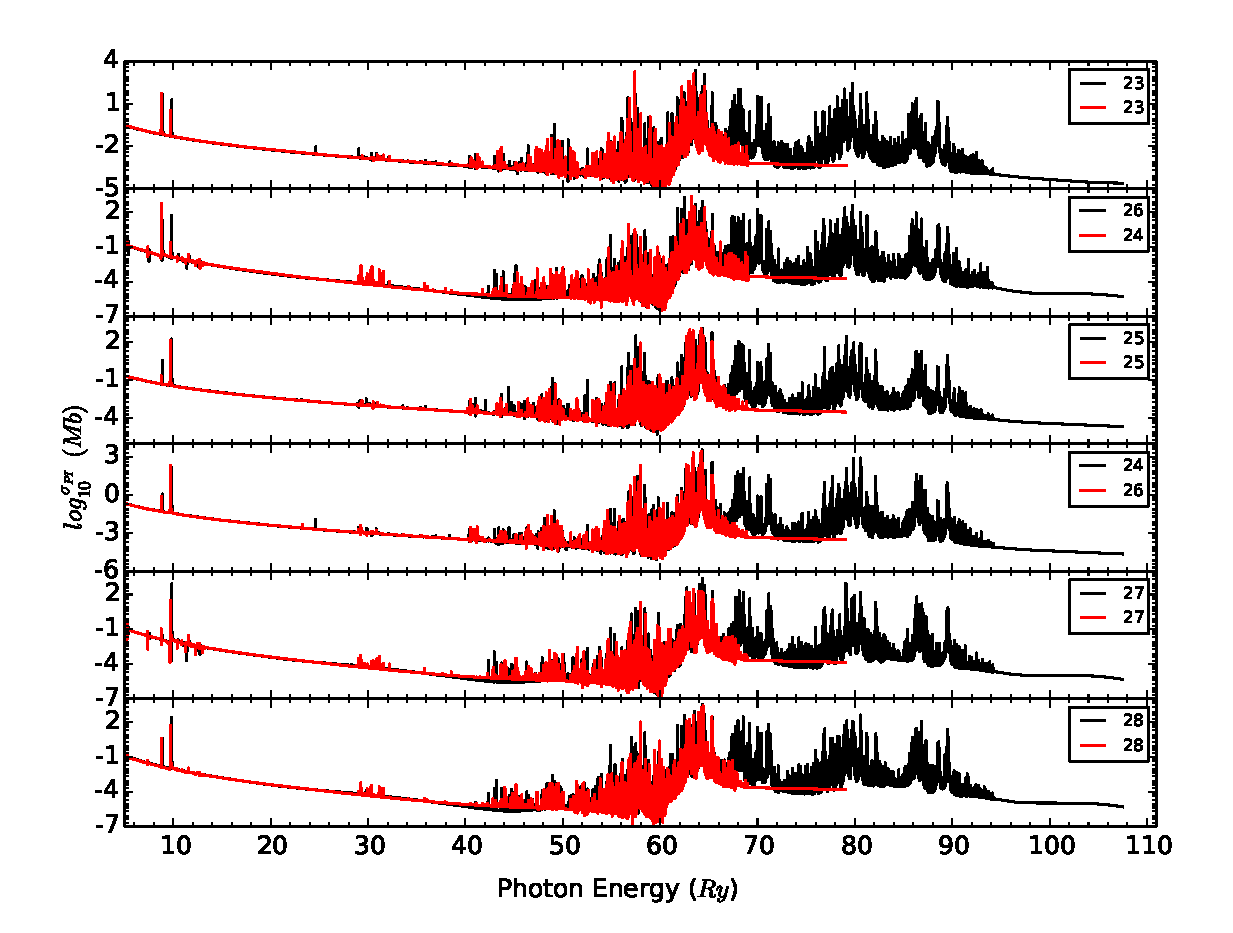
\includegraphics[width=0.49\textwidth]{figures/fe17_n3_n4_rematch}
		\label{fe17_n3_n4_rematch}
	}
~
	\subfloat[\ion{Fe}{xviii}: after level 31 and 33 being switched]{
		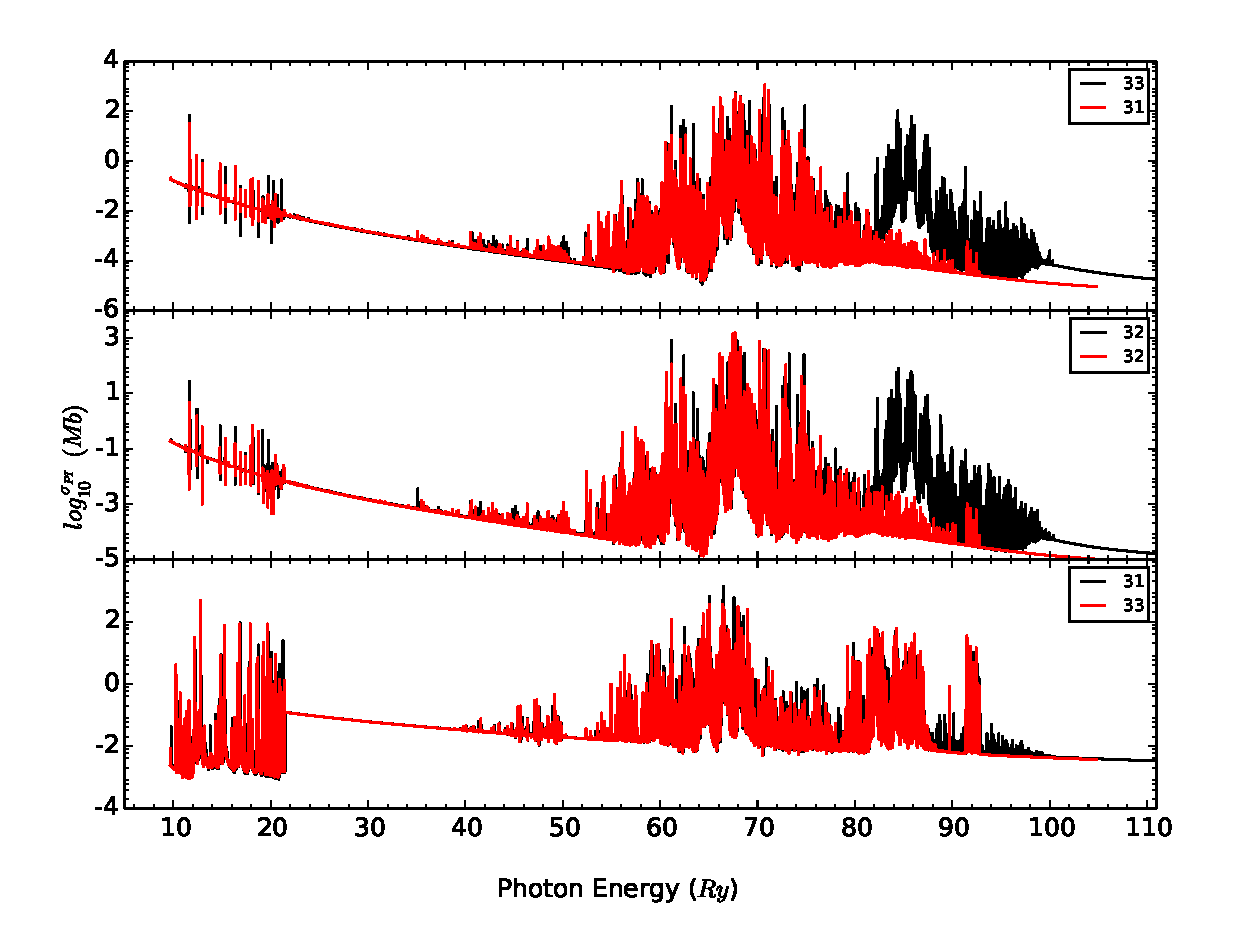
\includegraphics[width=0.49\textwidth]{figures/fe18_n3_n4_rematch}
		\label{fe18_n3_n4_rematch}
	}
	\caption{Photoionization cross section of 6 closely packed levels for \ion{Fe}{xvii} and 3 levels for \ion{Fe}{xviii} before and after being swtiched. \subref{fe17_n3_n4_mismatch}, \subref{fe18_n3_n4_mismatch}:  60CC-BPRM (red), 218CC-BPRM (black); \subref{fe17_n3_n4_rematch}, \subref{fe18_n3_n4_rematch}: 200CC-BPRM (red), 276CC-BPRM (black)}
	\label{mismatch}
\end{figure}

%=========== 3. TOPUP
\section{Top-Up}
Opacity project \citep{opcd_1, opcd_2} used close-coupling approximation and $R$-Matrix method to calculate photoionization cross section in the low energy region, and adopted a Kramer approximation fit afterwards \citep{opcd_7}. \citet{zhang_1998} replaced the Kramer tails with the relativistic distorted wave results including the contribution from inner-shell processes. Later opacity talbes were updated through including inner-shell transitions calculated by AUTOSTRUCTURE \citep{config_2003, config_2005}. In this section, we describe the procedure employed to match the bound state levels from BPRM and FAC calculations, and detail the bound-bound and bound-free top up calculation. Along the way, we discuss the effect of configuration interaction on the photoionization cross section. 

In diagram \ref{figure_topup_graph}, the black lines on the left indicate the core states that are already included in BPRM calculation, and the black lines on the right indicate the bound and quasi-bound levels that are considered in BPRM calculation. So the topup work is to include other core states up to principal quantum number $n=10$ (red lines on the left), and other pure bound levels (red lines indicated below $E=0$). For the bound levels that are already included in BPRM calculation, we first need to extend the calculation of direct photoionization to $500Ry$, then add the contribution due to the red lines on the left. For the unincluded bound levels, we need to calculation the direct photoionization due to all the core states. To simulate the autoionization resonances, we calculate the oscillator strength from the pure-bound levels to the red quasi-bound levels on the right. In addition we also include the bound-pure-bound transitions involving the unincluded bound levels (red lines below  $E=0$).
%======= FIGURE: topup_graph
\begin{figure}
	\centering
	\includegraphics[width=.9\textwidth]{figures/topup_graph}	
	\caption{A diagram showing where the topup is done. Red: untreated in BPRM calculation; black: treated in BPRM calculation.}
	\label{figure_topup_graph}
\end{figure}

\subsection{Matching} \label{section_matching}
In BPRM calculation, the continuum orbitals $\ell\leq9$, the effective quantum number $\nu\leq10.1$, and the bound state levels can only be formed by coupling the $n=2$ core states with the continuum orbitals. So in FAC, we set the bound configurations as a permutation of the $n=2$ core configurations and an outer electron with principle quantumn number $n\leq10$. With only the same n-complex configuration interaction included, atomic structure is solved, sorted by total angular momentum $J$ and parity $\pi$, and ordered in energy, we find excellent agreement in the enregy between BPRM and FAC.

In calculating photoionization cross section, we include the whole n-complex of the core configurations for configuration interaction purpose, but only the transitions to the core configurations that are included in BPRM calculation are calculated. To delineate the edges of the photoionization cross section, the energy mesh is created in such a way that within any adjacent thresholds, 10 points are uniformly assigned. The partial photoionization cross section is computed in the default 6 energy grids, and interpolated/extrapolated in our mesh, and summed to give the toal photoionization cross section for each bound state level. To investigate the effect of configuration interaction on the photoionization cross section, two sets of RDW calculation are carried out. Both sets only allow the same-n-complex configuration interaction for bound configurations, but for the core configurations, one of them only allows the same-n-complex configuration interaction, and the other allows different-n-complex configuration interaction and we mix all the core configurations together. In RDW calculation, the photoionization strength is the dipole operator matrix $<\psi_i|\mathbb{D}|\psi_f>$ involving the electron in the bound state to the continuum, and all other electrons in the $|\psi_i>$ and $|\psi_f>$ must stay the same if only same-n-complex configuration inteaction is allowed, and can be different if different-n-complex configuration interaction is considered \citep{gu_email}.

To match the bound state levels from BPRM and RDW, it's necessary to compare the photoionization cross section to ensure the correctness of matching. We plot the photoionization cross section of BPRM and RDW in the order of energy for each $J$, $\pi$ symmetry pair, and a level is matched when the energy and the photoionization cross section agree reasonably well (here the background of the BPRM data and RDW are compared). Even though the different-n-complex configuration interaction for core configurations is used to maximally reproduce the background of BPRM calculation, we use the energy of the ground state of $n=2$ core when same-n-complex configuration interaction is applied as a reference to calculate the energy of the bound levels, as we found in this way RDW gives energies that are more close to BPRM's results. The photoionization cross section of the majority of the bound levels shows excellent consistancy at the first attempt (see figure \ref{fe17_bprm_fac} for \ion{Fe}{xvii} and figure \ref{fe18_bprm_fac} for \ion{Fe}{xviii}, where term notation ( $S$ and $L$) can not be determined from FAC output for all levels, so only configuration and total angular momentum $J$ are given). However, when several levels have almost the same energy (see table \ref{table_levles_matching}), distinctive difference may occur in the photoionization cross section and these levels need to be switched till good matching is achieved  (See figure \ref{fe17_howtomatch} for \ion{Fe}{xvii} and figure \ref{fe18_howtomatch} for \ion{Fe}{xviii}. Note: all the photoionization cross section of BPRM calculation includes a small region below the lowest ionization threshold for each level \citep{opcd_4}, where no RDW data is shown. ). In table \ref{table_levles_matching}, we can see the energy levels computed in BPRM and RDW agree quite well. For \ion{Fe}{xvii}, levels 13 and 14 , and levels 15 and 16 lie very close to each other, and in figure\ref{fe17_howtomatch}, levels 13 and 16 achieve good agreement, while levels 14 and 15 do not. So we switch the order of levels 14 and 15 in RDW calculation and recompare. Good agreement is achieved. Thus levels 13 - 16 in BPRM calculation are matched with those in RDW calculation. The same procedure is applied to levels 65 and 66 of \ion{Fe}{xviii} in table \ref{table_levles_matching}, and the result is shown in figure \ref{fe18_howtomatch}. When several levels are closely lying together and their BPRM photoionization cross section data are almost indistinguishable, exact matching in this way is lack of confidence, and the top up calculation performed on these levels may not correctly add the right tail to BPRM data (see section \ref{section_tail}), or add the contribution from the correct other-core configurations to the tailed BPRM data (see section \ref{section_other_targets}), but this will not make an impact in the opacity calculation as these levels have the same symmetry, almost the same energies, and almost the same photoionization cross section.

Usually it is rare to have more levels found in BPRM than that in RDW in the corresponding region, because BPRM does this by scanning the effective quantum number with a scanning step \citep{seaton_bound_1985, berrington_seaton_1985}, so it is possible that some of the levels that have very similar effective quantum number are missed out by such scanning technique, while RDW does an atomic structure calculation, i.e. including all the possible levels formed by electron quantum number coupling. However, such peculiar case happens in symmetry $J = 7/2, \pi = o$ of \ion{Fe}{xviii}. See table \ref{table_fake_level}. Around energy of $-3.5*z^2*10^{-2} Ry$, where $z=18$, BPRM finds 3 levels by scanning, while RDW gives only 2 levels. And we can see that levels 27 and 28 only differ by the last digit. Checking their photoionization cross section (see figure \ref{figure_fake_level}), we can hardly find any difference between levels 27 and 28. Thus we believe that one of levels 27 and 28 is spurious, and it may be caused by the numerical errors in BPRM. However, without deeper investigation, we still took it in the opacity calculation. Thus, in symmetry $J = 7/2, \pi = o$, from level 29 (we chose 29, but it is better 28)on, level $i$ in BPRM is matched with level $(i-1)$ in RDW. Therefore, from this point of view, level shifting is crucial and photoionization cross section comparison is necessary when doing the level matching. 

For both \ion{Fe}{xvii} and \ion{Fe}{xviii}, all bound levels are matched between BPRM and RDW, with excellect agreement. But in symmetry $J = 17/2, \pi = e$ of \ion{Fe}{xviii}, there is a big gap in the energy region where no dense resonances appear. The reason for this is that in BPRM calculation, only symmetries $J = 15/2, \pi = e$ and $J = 17/2, \pi = e$ of the free states are considered (no information about $J = 19/2, \pi = e$ in stg2), thus the photoionization cross section in BPRM is lower. For a complete view of the comparasion of the photoionization cross section (with the right oscillating end removed in BPRM data, see section \ref{section_tail}), go to \url{https://github.com/zhao1157/PhD-Atomic-Physics/tree/master/fe17_fe18_matched_levels}. 

%========= Table fake levels 7_1_27-28
\begin{table}
	\centering
	\caption{\ion{Fe}{xviii}: In symmetry $J = 7/2,~\pi = o$ of \ion{Fe}{xviii}, around energy $-3.5$, BPRM finds 3 levels, while RDW gives 2 levels. Note: the energy is $z$-scaled, and in unit of $10^{-2} Ry$.}
	\begin{tabular}{|c|c|}
		\hline
		\multicolumn{2}{|c|}{BPRM} \\
		\hline
		index & energy \\	
		\hline
		26 & -3.657952 \\
		27 & -3.523161 \\
		28 & -3.523163 \\
		29 & -3.522445 \\
		30 & -3.101211 \\	
		\hline	
	\end{tabular}
	\quad
	\begin{tabular}{|c|c|}
		\hline
		\multicolumn{2}{|c|}{RDW} \\
		\hline
		index & energy \\	
		\hline
		26 & -3.63053 \\
		27 & -3.53045 \\
		28 & -3.52958 \\
		29 & -3.11294 \\
		30 & -2.92945 \\	
		\hline	
	\end{tabular}
	\label{table_fake_level}
\end{table}

%======= FIGURE: 7_1_27-28 fake levels
\begin{figure}
	\centering
	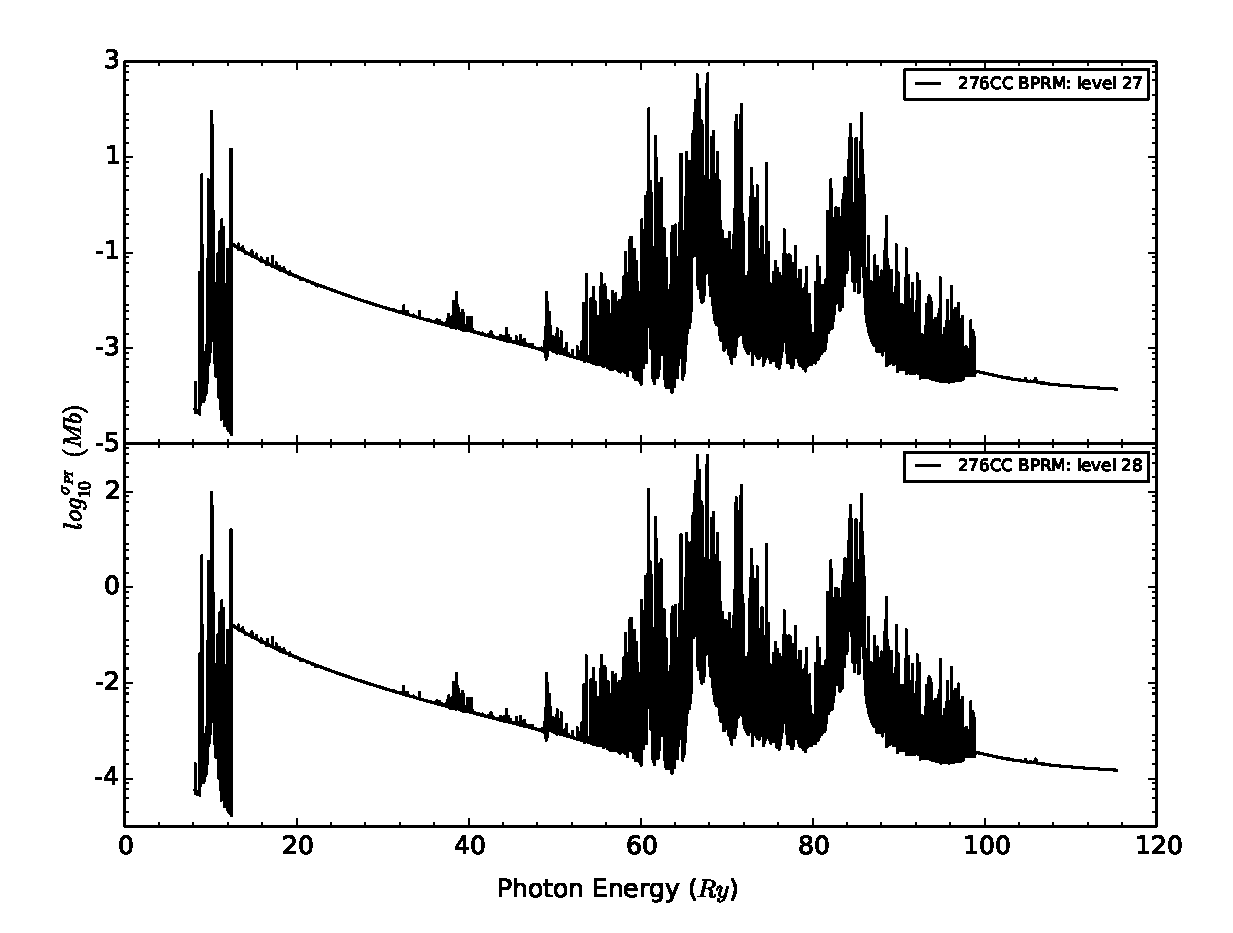
\includegraphics[width=.9\textwidth]{figures/fe18_fake_levels.eps}	
	\caption{\ion{Fe}{xviii}: The photoionization cross section of levels 27 and 28 as shown in table \ref{table_fake_level}.}
	\label{figure_fake_level}
\end{figure}




In figures \ref{fe17_bprm_fac}, \ref{fe18_bprm_fac}, \ref{fe17_howtomatch} \ref{fe18_howtomatch}, we show two sets of RDW calculation as described above and study the effect of configuration interaction on the photoionization cross section. Take the upper panel of figure \ref{fe17_bprm_fac} as an example. The configuration of the bound state after being matched with RDW is $2s^2 2p^5 4d$, so with only same-n-complex configuration interaction of the core configurations considered, the transitions can only happen to core configurations $2s^2 2p^5$, $2s 2p^5 4\ell$, $2s^2 2p^4 4\ell$ and $2p^6 4\ell$, where $\ell=s, p, d$, while with different-n-complex configuration interaction of the core configurations considered, additional contribution can be from all other core configurations. From  the upper panel of figure \ref{fe17_bprm_fac} we can see that same-n-complex configuratoin interaction gives pretty good background, though with some big gaps, while different-n-complex configuration interaction fills up such a big gap and improves the background significantly. The similar phenomenon can be found in the rest of the figures  \ref{fe17_bprm_fac}, \ref{fe18_bprm_fac}, \ref{fe17_howtomatch} \ref{fe18_howtomatch}, and there are still some gaps remaining after different-n-complex configuration interaction is allowed (Note: in figure \ref{fe18_bprm_fac} and \ref{fe18_howtomatch}, the oscillation in the background of the BPRM data can be eliminated with a larger number of continuum basis functions \citep{zhang_1998}).

Before deciding considering the different-n-complex configuration interaction of only the core configurations, we did the RDW calculation with different-n-complex configuration interaction of the bound configurations, i.e. putting all the bound configurations in just one $Structure()$ funciton in FAC. The result is not good when compared with BPRM result. Take levels 3 and 18 in symmetry $J=0,~\pi=e$ of \ion{Fe}{xvii} as an example. In figure \ref{figure_fe17_bound_mix}, we can see that with only same-n-complex configuration interaction of the bound configurations, RDW gives great result, while different-n-complex configuration interaction of the bound configurations makes the lower energy transitions worse. Thus in the level-matching process, to be consistent with BPRM result, we only consider the same-n-complex configuration interaction for the bound configurations, and different-n-complex configuration interaction for the core configurations. So is it in the top up calculation. 


%======== TABLE: closely packed levels in matching ======
\begin{table}
	\centering
	\caption {Selected levels of \ion{Fe}{xvii} ($J = 3, \pi = e$) and \ion{Fe}{xviii} ($J=1/2, \pi=e$) to be matched (Note: the energy is $z$-scaled, and in unit of $10^{-2} Ry$)}
	\begin{tabular}{|c || c | c | c|}
		\hline
		& level index & BPRM & RDW \\
		\hline
		\multirow{6}{*}{\ion{Fe}{xvii}} & 12 & -3.670657 & -3.67960 \\
		& 13 & -2.873930 & -2.84319 \\
		& 14 & -2.868775 & -2.84238 \\
		& 15 & -2.842915 & -2.83761 \\
		& 16 & -2.835625 & -2.83555 \\
		& 17 & -2.774853 & -2.77998 \\
		\hline
		\hline
		& level index & BPRM & RDW \\
		\hline
		\multirow{4}{*}{\ion{Fe}{xviii}} & 64 & -1.275887 & -1.27703  \\
		& 65 & -1.234865 & -1.24175 \\
		& 66 & -1.226084 & -1.23724 \\
		& 67 & -1.136909 & -1.14691 \\
		\hline
	\end{tabular}	
	\label{table_levles_matching}
\end{table}



%======= FIGURE: bprm and fac match
\begin{figure}
	\centering
		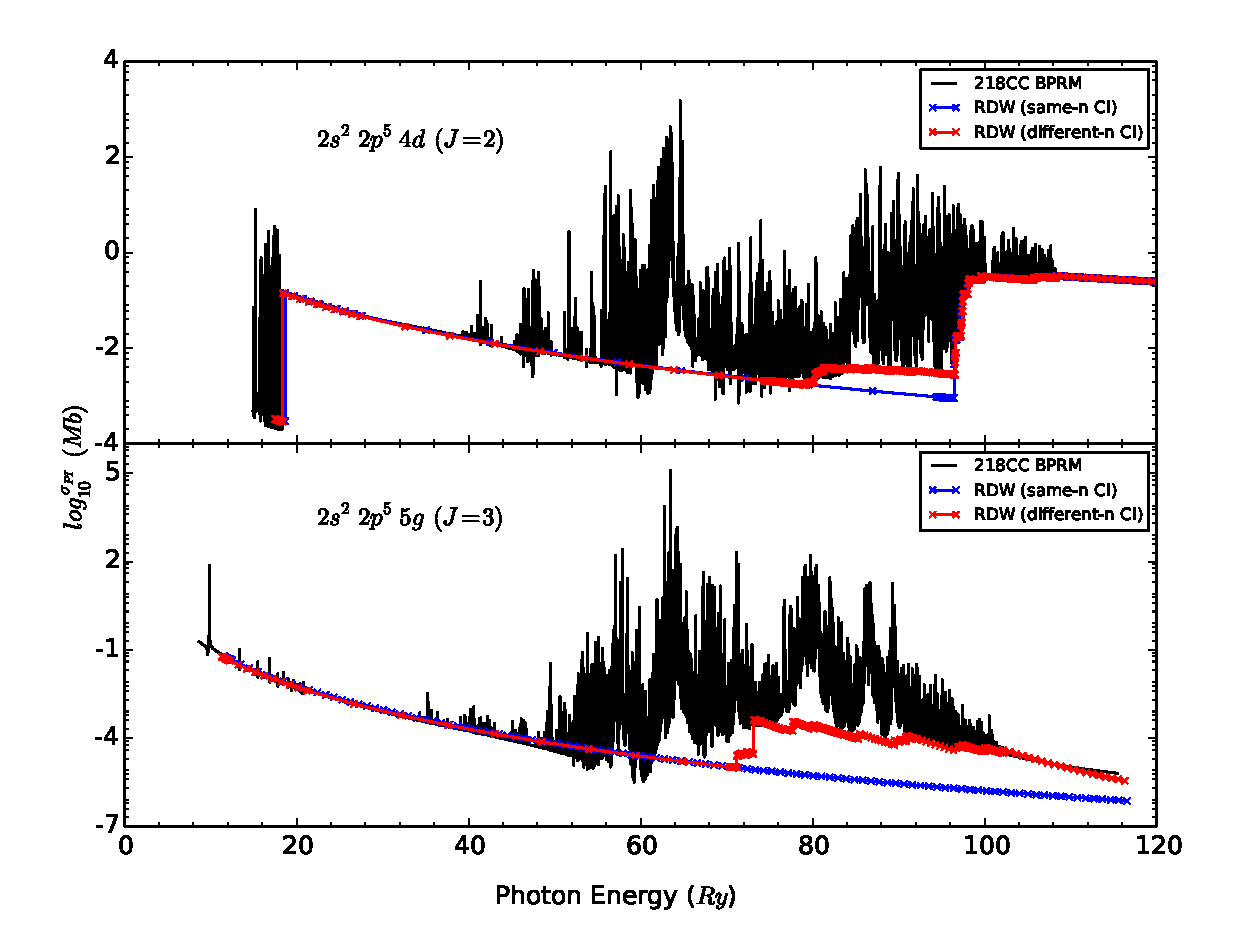
\includegraphics[width=.9\textwidth]{figures/fe17_bprm_fac.eps}	
	\caption{\ion{Fe}{xvii}: Most of the levels are matched at the first attempt with excellent consistency in photoionization cross section. The configuration is attached with each levle. BPRM (black), RDW(blue and red). ``Same-n CI'' means only same-n-complex configuration interaction is considered for core configurations, and ``different-n CI'' refers to both same-n- and different-n-complex configuration interaction is considered.}
	\label{fe17_bprm_fac}
\end{figure}

\begin{figure}
	\centering
	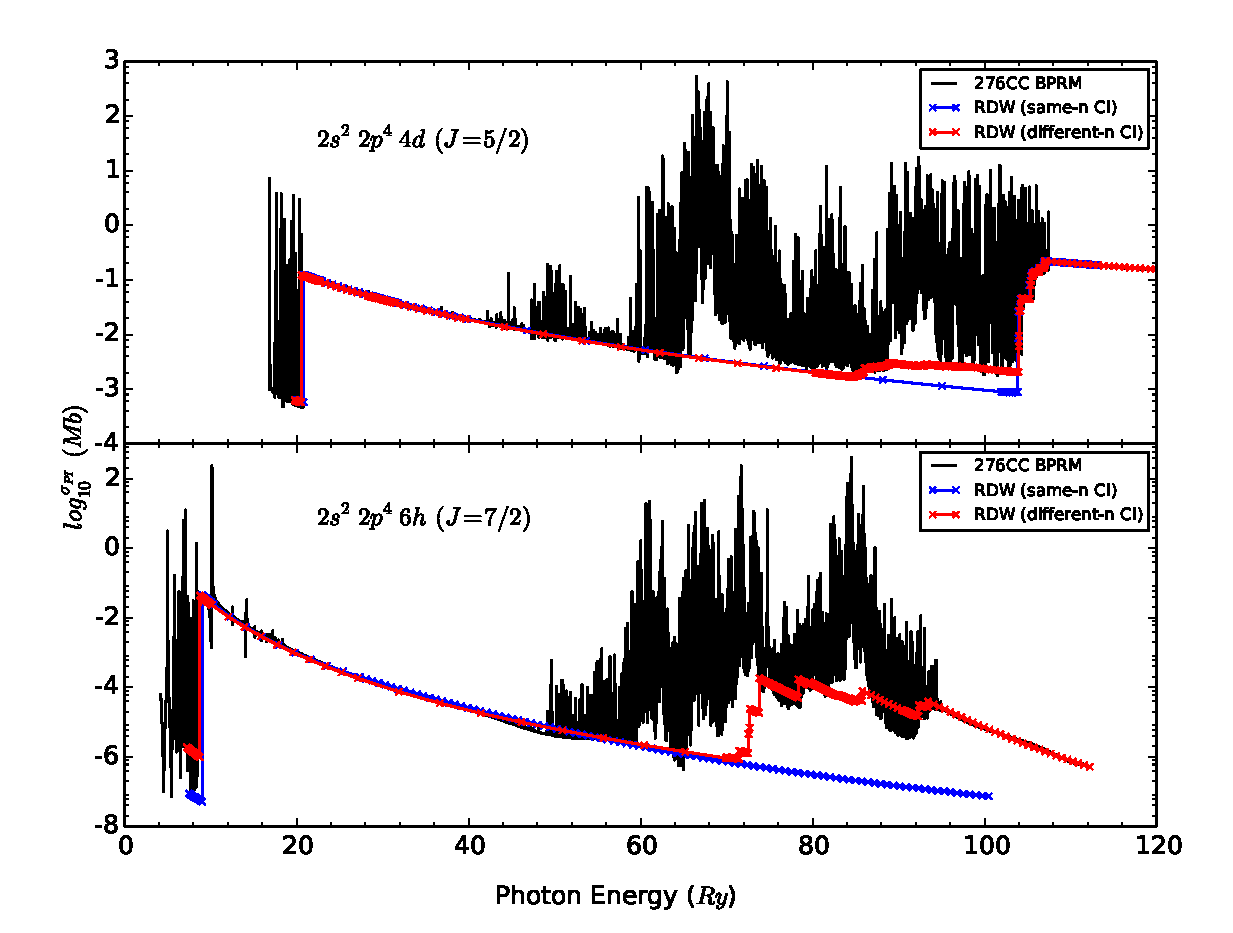
\includegraphics[width=.9\textwidth]{figures/fe18_bprm_fac.eps}
	\caption{\ion{Fe}{xviii}: Most of the levels are matched at the first attempt with excellent consistency in photoionization cross section. The configuration is attached with each levle. BPRM (black), RDW(blue and red). ``Same-n CI'' means only same-n-complex configuration interaction is considered for core configurations, and ``different-n CI'' refers to both same-n- and different-n-complex configuration interaction is considered.}
	\label{fe18_bprm_fac}
\end{figure}

%=========Figure: HOWTOMATCH
\begin{figure}
	\centering
	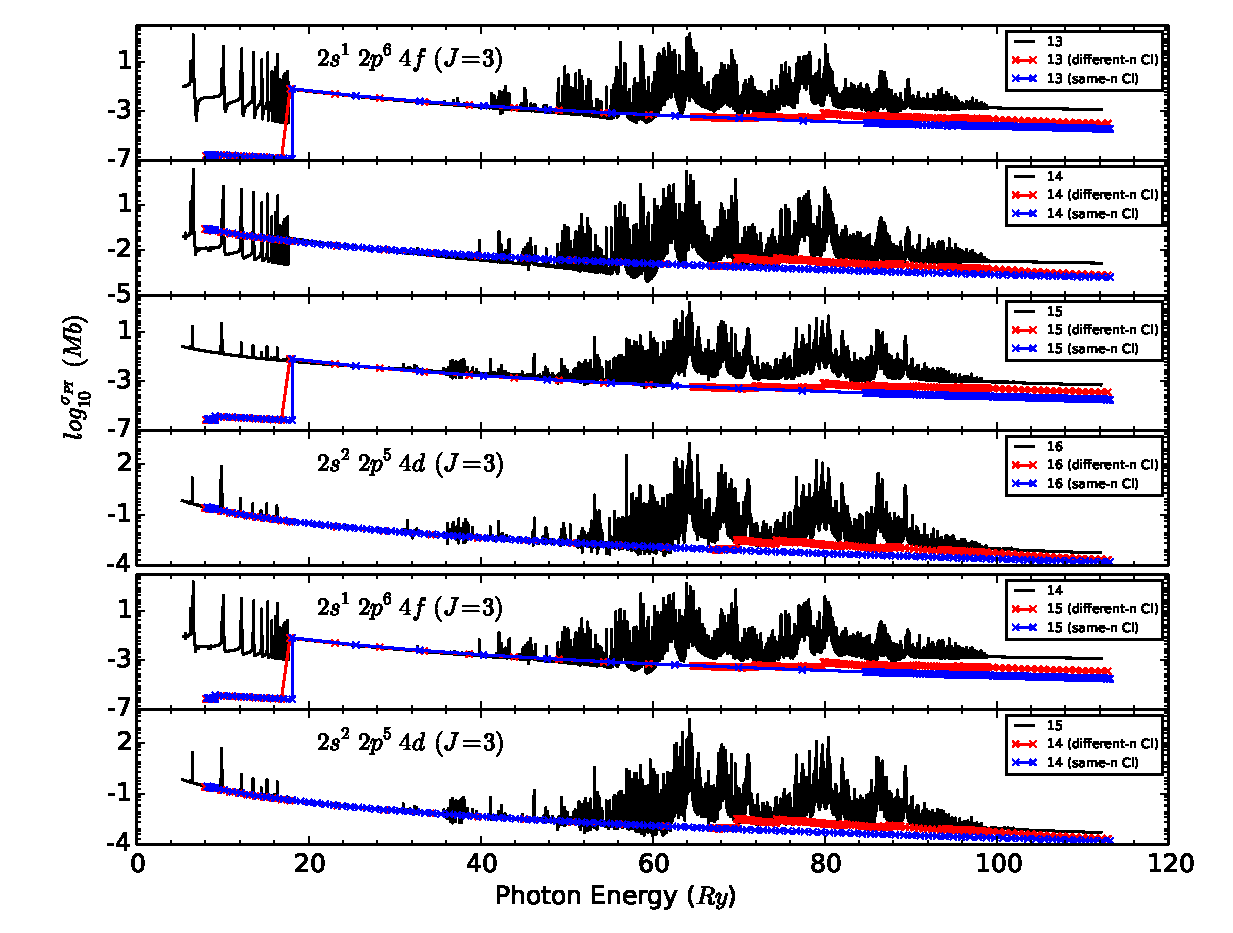
\includegraphics[width=.9\textwidth]{figures/fe17_howtomatch.eps}
	\caption{\ion{Fe}{xvii}: Multiple attemps are needed to ensure the correct matching when the levels are found with discrepancy in the photoionization cross section. The discrepancy is shown in upper panel and the final matching is in the lower one. Find the confuration attached for each level. BPRM (black), RDW(blue and red). ``Same-n CI'' refers to only same-n-complex configuration interaction is considered for core configurations, and ``different-n CI'' refers to both same-n- and different-n-complex configuration interaction are considered.}
	\label{fe17_howtomatch}
\end{figure}

\begin{figure}
	\centering
		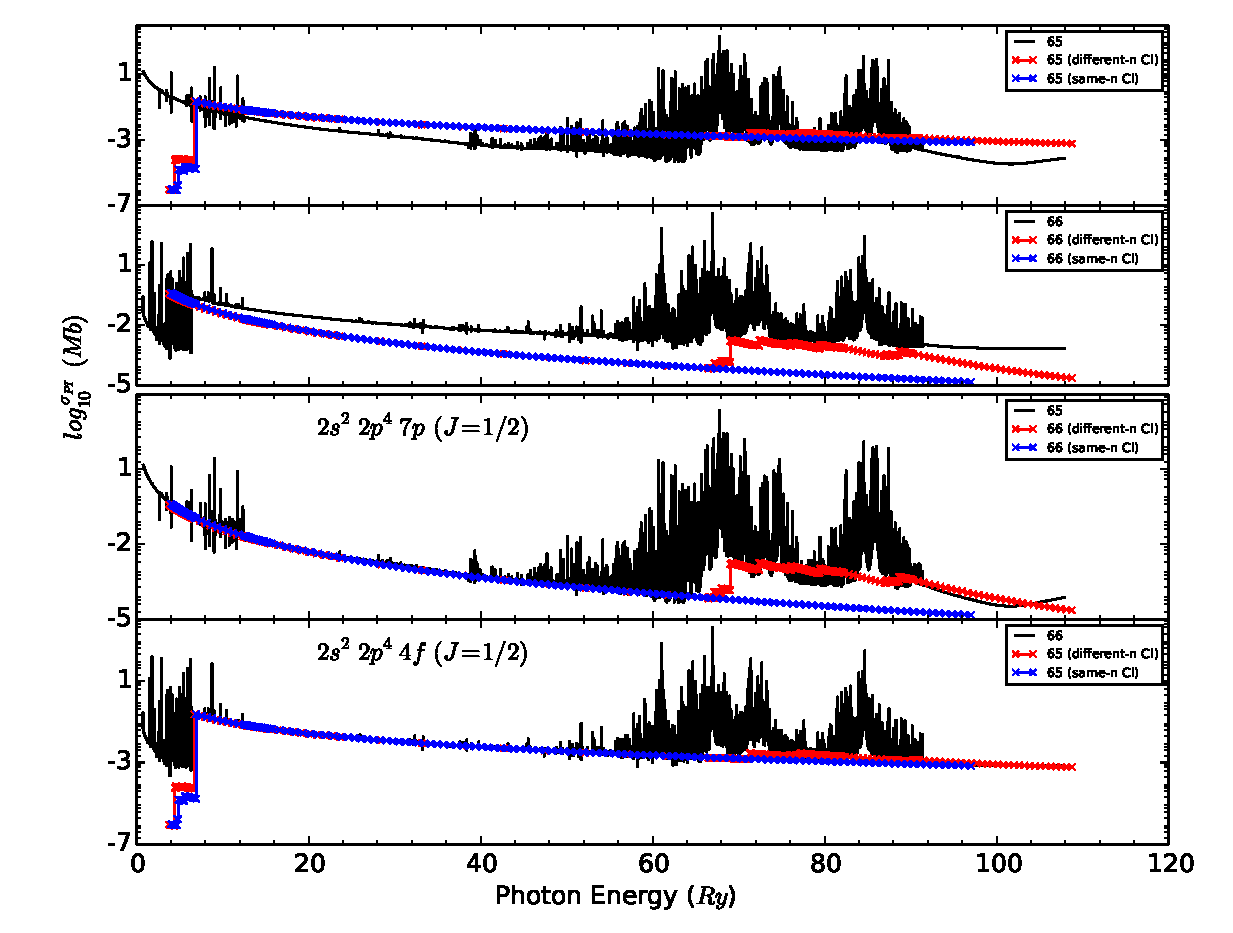
\includegraphics[width=.9\textwidth]{figures/fe18_howtomatch.eps}
	\caption{\ion{Fe}{xviii}: Multiple attemps are needed to ensure the correct matching when the levels are found with discrepancy in the photoionization cross section.The discrepancy is shown in upper panel and the final matching is in the lower one. Find the confuration attached for each level. BPRM (black), RDW(blue and red). ``Same-n CI'' refers to only same-n-complex configuration interaction is considered for core configurations, and ``different-n CI'' refers to both same-n- and different-n-complex configuration interaction are considered.}
	\label{fe18_howtomatch}
\end{figure}

%=========Figure: bound configurations mix
\begin{figure}
	\centering
	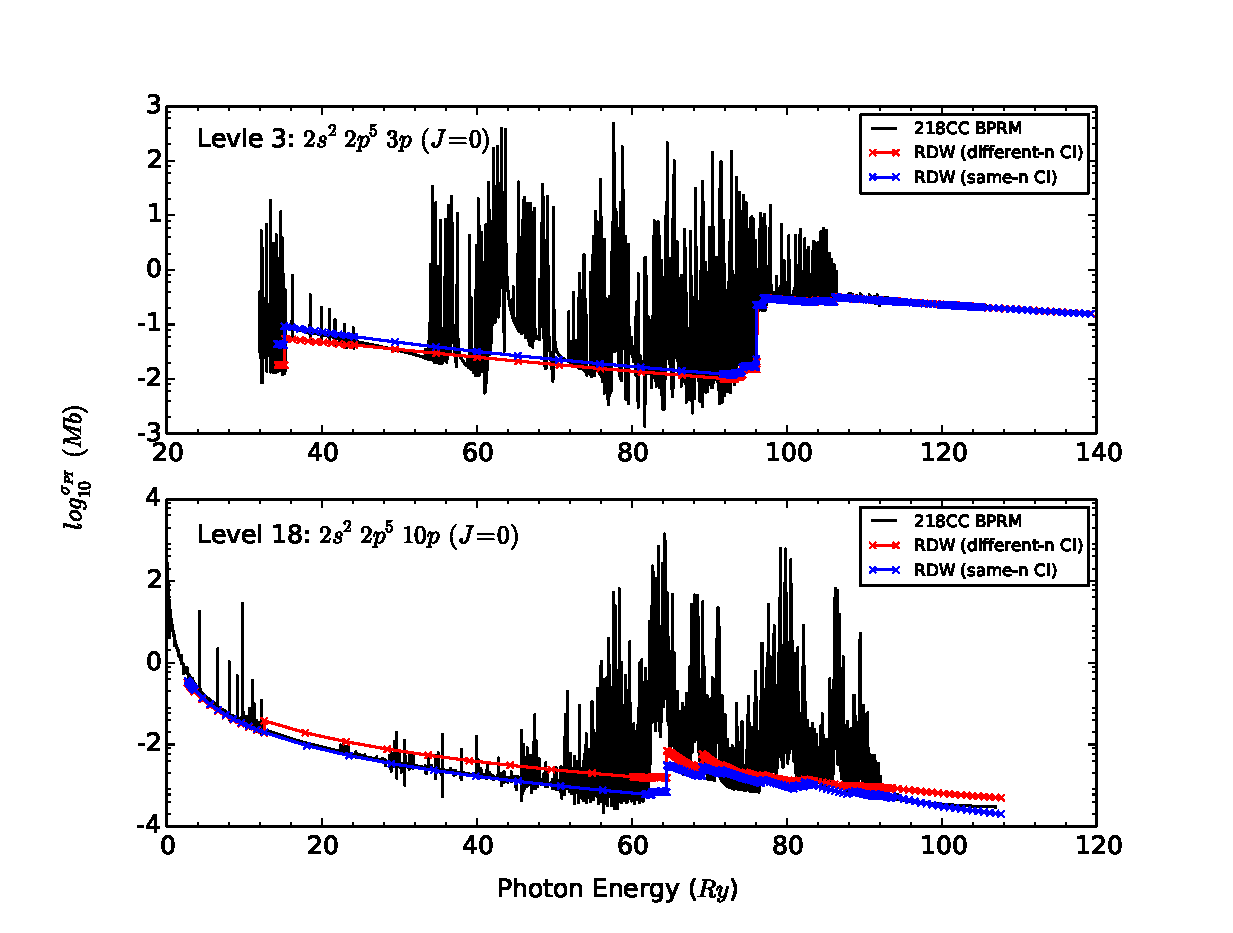
\includegraphics[width=.9\textwidth]{figures/fe17_bound_mix.eps}
	\caption{\ion{Fe}{xvii} ($J = 0, ~\pi=e$): BPRM (black), RDW(blue and red). In addition to the different-n-complex configuration interaction of the core configurations included, the configuration interaction of the bound configurations is tested.  ``Same-n CI'' refers to only same-n-complex configuration interaction is considered for the bound configurations, and ``different-n CI'' refers to both same-n- and different-n-complex configuration interaction are considered.}
	\label{figure_fe17_bound_mix}
\end{figure}


\subsection{Bound - Free} \label{section_bf}
As BPRM calculation is carried out in the lower part of the whole energy range, and it inlucdes low-n core configurations, we use RDW to extend it to higher region up to 500 $Ry$ of photoelectron energy, and to include high-n core configurations up tp $n=10$. The following part of the section gives detailed description of these aspects.

\subsubsection{Tail} \label{section_tail}
As shown in figures \ref{fe17_bprm_fac} and \ref{fe18_bprm_fac}, the RDW data can be matched almost perfectly to the background of BPRM result, however, we also find there are cases where they do not match well in the right region of energy. For example, in the top panels of figures \ref{fig_fe17_discrepancy} and \ref{fig_fe18_discrepancy}, different-n-complex CI introduces many transitions, but they are not strong enough to raise to the  background of BPRM. In the middle panel of figure \ref{fig_fe17_discrepancy}, different-n-complex CI introduces many edges at positions where the background of BPRM jumps, and raises the background higher than BPRM. While in the middle panel of figure \ref{fig_fe18_discrepancy}, around $105~Ry$, compared with same-n-complex CI, different-n-complex CI moves the background up on the left side, and down on the right side, i.e. converging to the background of BPRM.

Initially as only the same-n-complex CI was considered, there were big gaps between the background of BPRM and RDW for majority of the bound levels, and to extend the data to higher energy region, we multiplied the RDW data for each level by a ratio obtained at the last point of BPRM so that the values of BPRM and RDW are equal at that energy. When different-n-complex configuration interaction is considered, such big gaps are mostly filled up, though with some discrepancy for some levels, the same ``scaled-RDW'' tail treatment is applied and the distribution of the ratios are shown in figure \ref{fig_ratio} for both \ion{Fe}{xvii} and \ion{Fe}{xviii}. We can see that the distribution is very alike for both ions, and there are around $60\%$ of the bound levels lying around ratio of 1, and the rest are in high ratios. After further investigation, we find the high ratios are mainly caused by the oscillation of BPRM background, which is due to the small number of continuum basis funcitons used in the wavefunction expansion \citep{zhang_1998}. Please see the bottom panels of figures \ref{fig_fe17_discrepancy} and \ref{fig_fe18_discrepancy}. With such oscillation removed at the end of BPRM data (about the last 1000 points for each level), the ratios improve dramatically (see figure \ref{fig_ratio_no_oscillation}), and there are about $85\%$ of the levels are around ratio of 1. Through this distribution, we can have a glimpse of how well the levels are matched and how well the BPRM and RDW calculation agree with each other. But with further consideration, we set all the ratios to 1, i.e. take RDW data as it is, and add RDW tail directly to BPRM data just like what \citet{zhang_1998} did, because RDW is more accurate in the higher energy region and multiplying a ratio to RDW data introduces an obvious inaccuracy in that region, though without multiplying the ratio it causes a discontinuity in the data.

The energy mesh used in the region is created in such a way that 10 points are uniformly assigned beween any adjacent ionization thresholds due to the other core configurations (see section \ref{section_other_targets}).

%=========Figure: MATCH_DISCREPANCY
\begin{figure}
	\centering
	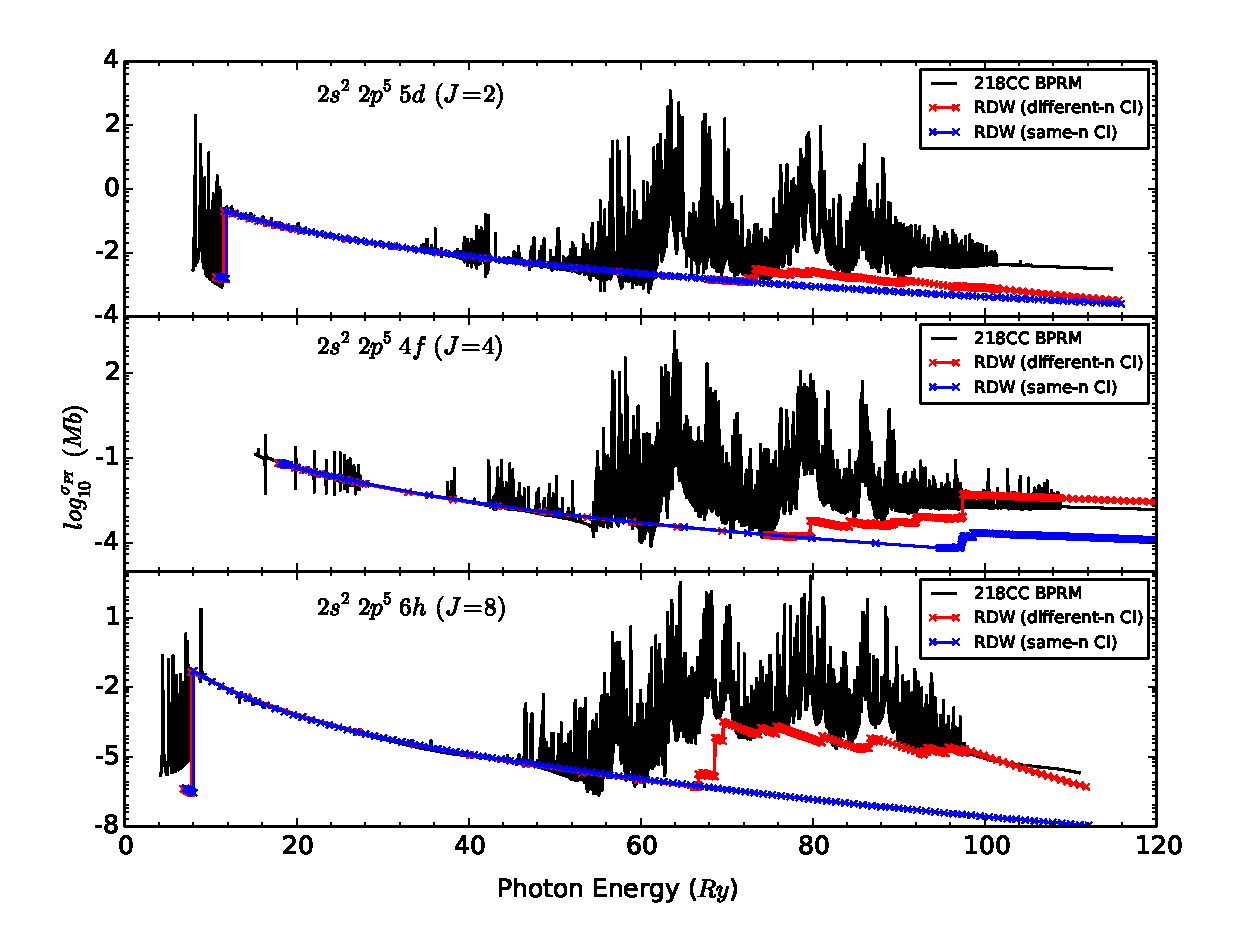
\includegraphics[width=.9\textwidth]{figures/fe17_discrepancy.eps}
	\caption{\ion{Fe}{xvii}: Different-n configuration interaction improves the background significantly, but there is still very large discrepancy in the right region of energy for some levels. BPRM (black), RDW(blue and red). ``Same-n CI'' refers to only same-n-complex configuration interaction is considered for core configurations, and ``different-n CI'' refers to both same-n- and different-n-complex configuration interaction are considered.}
	\label{fig_fe17_discrepancy}
\end{figure}

\begin{figure}
	\centering
	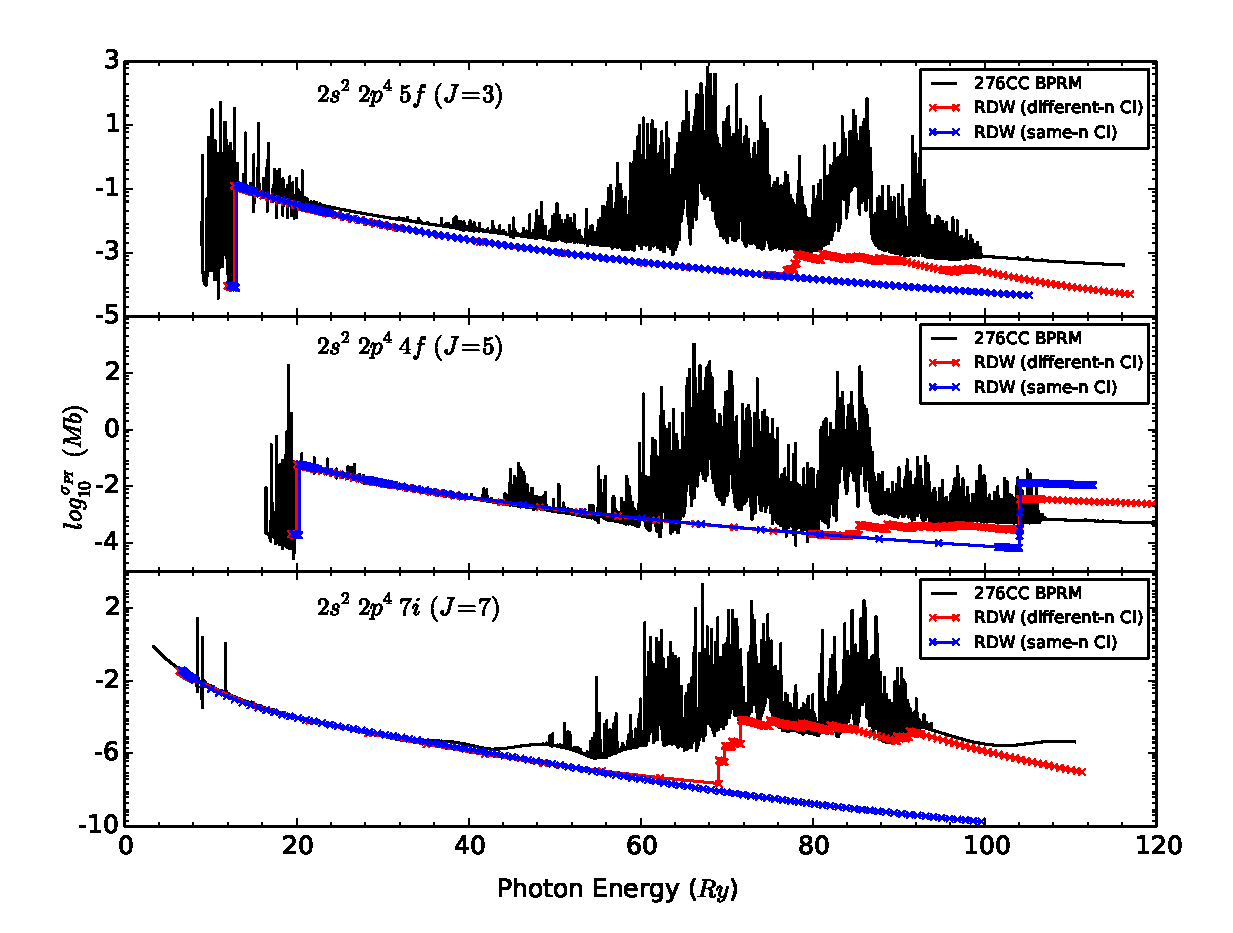
\includegraphics[width=.9\textwidth]{figures/fe18_discrepancy.eps}
	\caption{\ion{Fe}{xviii}: Different-n configuration interaction improves the background significantly, but there is still very large discrepancy in the right region of energy for some levels. BPRM (black), RDW(blue and red). ``Same-n CI'' refers to only same-n-complex configuration interaction is considered for core configurations, and ``different-n CI'' refers to both same-n- and different-n-complex configuration interaction are considered.}
	\label{fig_fe18_discrepancy}
\end{figure}

%=========Figure: RATIO with oscillation
\begin{figure}
	\centering
	\includegraphics[width=0.9\textwidth]{figures/ratio_bprm_fac.eps}
	\caption{The distribution of the factors multiplied to RDW data in the higher energy region for \ion{Fe}{xvii} and \ion{Fe}{xviii} with the oscillating end of BPRM data included. ``width'' is the width of the bins. }
	\label{fig_ratio}
\end{figure}

%=========Figure: RATIO with NO oscillation
\begin{figure}
	\centering
	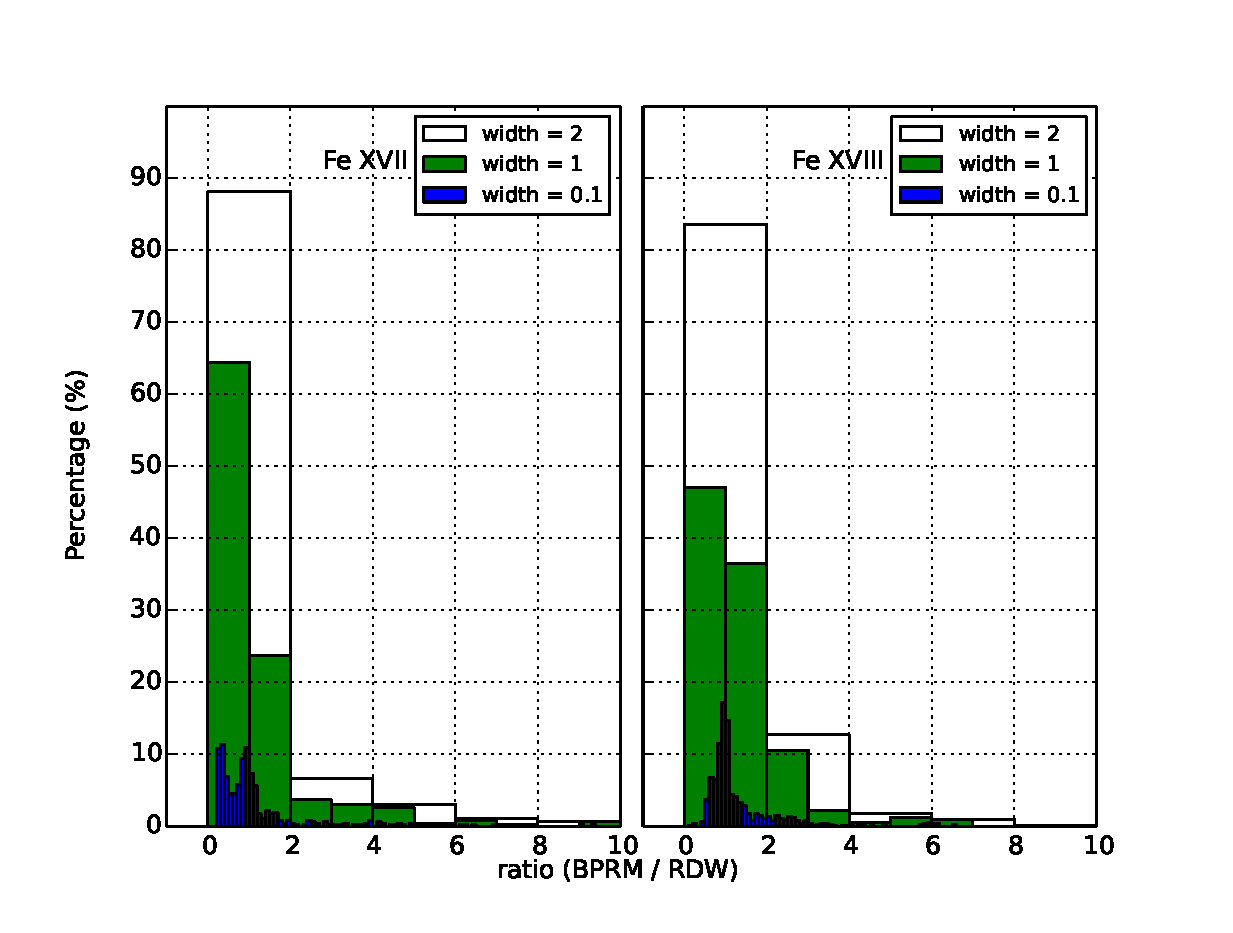
\includegraphics[width=0.9\textwidth]{figures/ratio_bprm_fac_no_oscillation.eps}
	\caption{The distribution of the factors multiplied to RDW data in the higher energy region for \ion{Fe}{xvii} and \ion{Fe}{xviii} \textbf{without} the oscillating end of BPRM data included. ``width'' is the width of the bins. }
	\label{fig_ratio_no_oscillation}
\end{figure}

\subsubsection{Other Core Configurations} \label{section_other_targets}
Using RDW with different-n-complex configuration interaction, we calculate photoionization cross section due to other core configurations up to $n=10$ that are not included in the BPRM calculation. As demonstrated in chapter \ref{chap_pec_l_edge}, the high-n core configurations are used to enable the convergence (jump) of the photoionization cross section of the high-n bound states. To top up 218CC BPRM for \ion{Fe}{xvii}, we include core configurations $2s^2 2p^4 4f$, $2s 2p^5 4f$, $2p^6 4\ell'$, and $2s^S 2p^P n\ell''$, where  $S$, $P$ are any possible non-negative integers satisfying $S+P=6$, $5 \leq n \leq 10$, and $\ell'$ and $\ell''$ are all possible subshells in the corresponding shell. To top up 276CC BPRM for \ion{Fe}{xviii}, we include core configurations $2p^5 3\ell$, $2s^2 2p^3 4f$, $2s 2p^4 4\ell'$,  $2p^5 4\ell''$,  $2s^S 2p^P n\ell'''$, where  $S$, $P$ are any possible non-negative integers satisfying $S+P=5$, $5 \leq n \leq 10$, and $\ell$, $\ell'$, $\ell''$ and $\ell'''$ are all possible subshells in the corresponding shell. The energy mesh is the same as the one used in BPRM calculation merged with the one in the high energy region as described in section \ref{section_tail}. 

As shown in figures \ref{fig_fe17_tail_other} and \ref{fig_fe18_tail_other}, the BPRM data is merged with the scaled RDW tail, and the contribution from other core configurations varies from negligible to noticeable. In table \ref{table_transition_other_core}, part of the transitions to the other core configurations are shown, which contribute most of the photoionizatoin cross section. Level $ 2s^2 2p^5 4d~(J=2) $ gets negligible contribution from the other core configurations compared with the tail, and the main transitions are due to different-n-complex configuration interaction. Levels $2s^2 2p^5 5g~(J=3)$, $2s^2 2p^4 4d~(J=5/2)$ and $2s^2 2p^4 6h~(J=7/2)$ have a good amount of contribution from the other core configurations, and they are mainly due to the same-n-complex configuration interaction, i.e. ionizing one electron from $L-$shell while keeping the other electrons unchanged. For level $2s^2 2p^4 4d~(J=5/2)$, since in 276 CCBPRM, core configuration $2s^2 2p^3 4d$ has been considered, leaving out $2s 2p^4 4d$, that is why only $2s 2p^4 4d$ contribute mainly in the top up calculation, and it is comparable with the BPRM tail, which is mainly due to the transitions to $2s^2 2p^3 4d$ (see table \ref{table_n3_n4_jumps}). 

To illustrate the statement made in section \ref{section_matching} that non-exact matching for closely lying levels does not make an impact on the accuracy of the top up data in terms of opacity calculation. Take level $2s^2 2p^4 6h~(J=7/2)$ as an example, which is level 44 as shown in table \ref{table_7_1_44}, in which levels 42 - 45 have almost the same energy and are distinctively different from levels 41 and 46, and once again BPRM and RDW calculations show a great agreement.  Figure  \ref{fig_7_1_44_not_matter} shows the photoionization cross section of these four levels, and we notice that even though those four levels have almost the same energy and the photoionization cross section look quite similar, levels 42 and 43 are more similar to each other while levels 44 and 45 look more similar to each other. It turns out levels 42 and 43 are from the same configuration $2s^2 2p^4 6f$ and levels 44 and 45 are from configuration $2s^2 2p^4 6h$. Thus for levels that have the same symmetry and very similar energy, the levels from the same configuration have very similar photoionization cross section, and it is impossible to distinguish them using our matching method. When doing the topup calculation, it does not matter which tail or contribution from other cores is added to which level among these indistinguishable levels. As shown in figure \ref{fig_7_1_44_not_matter_tail_other}, we can see that tails of levels 42 and 43 are essentially the same with negligible difference, so are the levels 44 and 45. And the contribution from other cores is also essentially the same. Thus there is really no need to distinguish them and the top up data is correctly added to the BPRM data.



%======== Table transitoins due to other cores
\begin{table}
	\centering
	\caption{Listed are some of the other core configurations which contribute most of the photoionization cross section for the four levles shown in figures \ref{fig_fe17_tail_other} and \ref{fig_fe18_tail_other}.}
	\begin{tabular} {|c ||c | c |}
		\hline
		Ion & Bound levels & Final configurations \\
		\hline
		\multirow{5}{*}{\ion{Fe}{xvii}} & \multirow{3}{*}{$2s^2 2p^5 4d~(J = 2)$} & $2s^2 2p^4 5d/5f/6d$ \\
																	   &  & $2s 2p^5 5d$ \\
																	   &  & $2p^6 4d$ \\
		\cline{2-3}
		&\multirow{2}{*}{$2s^2 2p^5 5g~(J = 3)$}  & $2s^2 2p^4 5g$ \\
																	   && $2s 2p^5 5g$ \\
		\hline
		\multirow{3}{*}{\ion{Fe}{xviii}} & \multirow{1}{*}{$2s^2 2p^4 4d~(J = 5/2)$}  & $2s 2p^4 4d$ \\
		\cline{2-3}
		& \multirow{2}{*}{$2s^2 2p^4 6h~(J = 7/2)$}  & $2s^2 2p^3 6h$ \\
																		 & & $2s 2p^4 6h$ \\
		\hline			  								   
	\end{tabular}
	\label{table_transition_other_core}
\end{table}

%=========Figure: TAIL_OTHER_TARGETS
\begin{figure}
	\centering
		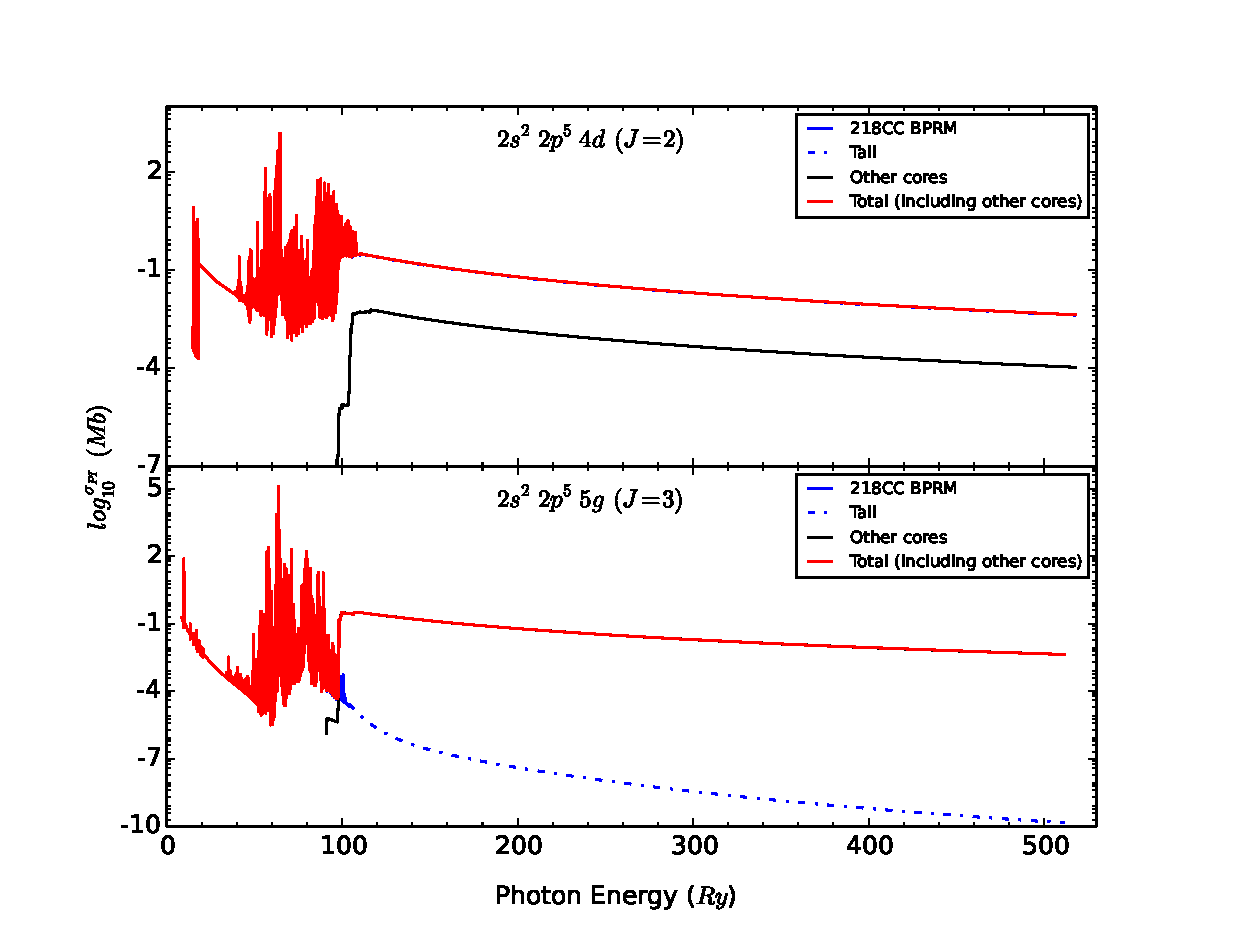
\includegraphics[width=.9\textwidth]{figures/fe17_tail_other_targets.eps}
	\caption{\ion{Fe}{xvii}: The photoinization cross section of the same four levels as in figure \ref{fe17_bprm_fac} are extended to higher enegy region and the contribution from other core configurations with different-n-complex configuration interaction is added. Blue (solid): BPRM calculation; blue (dash-dotted): RDW data; black: contribution from other core configurations; red: total photionization cross section.}
	\label{fig_fe17_tail_other}
\end{figure}

\begin{figure}
	\centering
		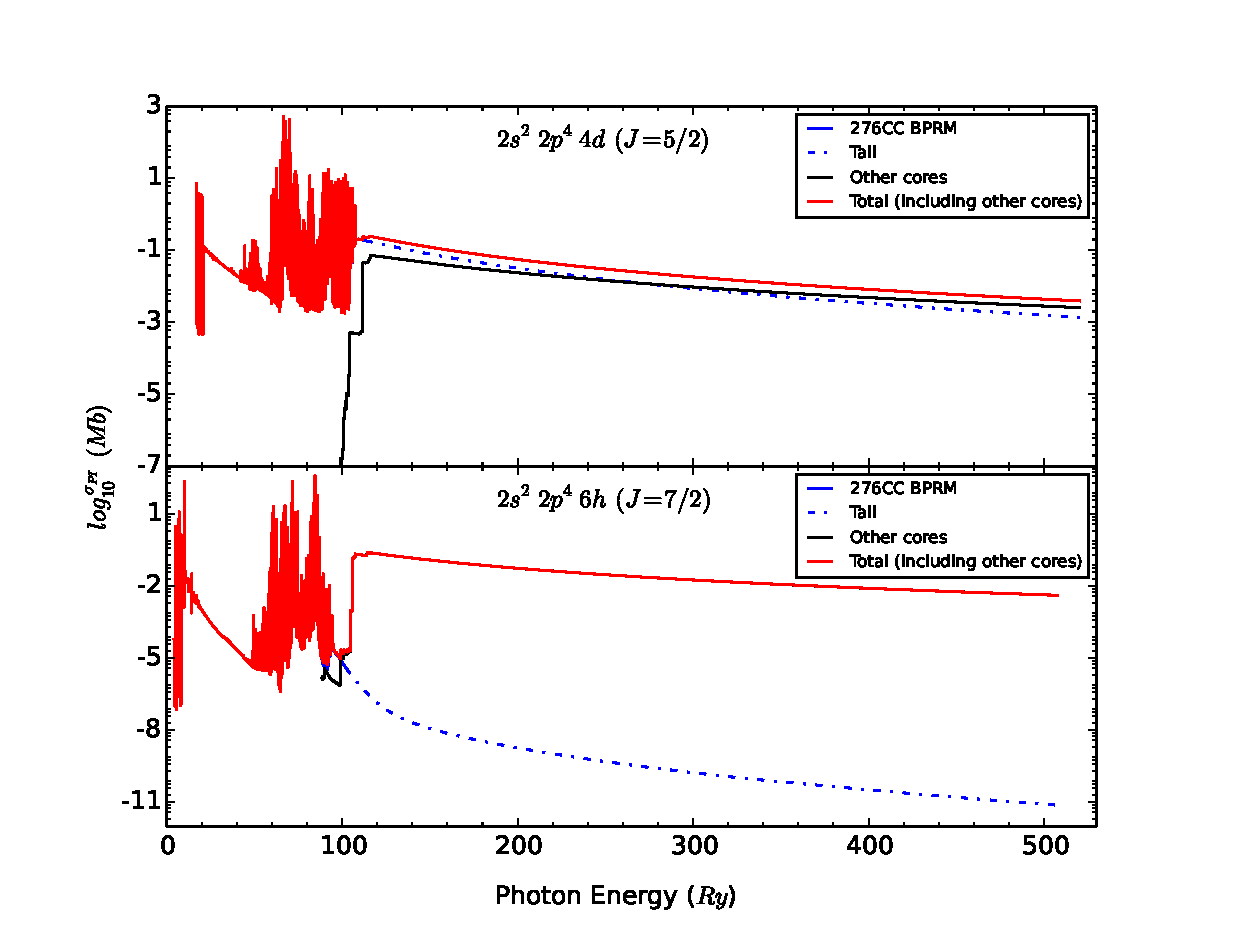
\includegraphics[width=.9\textwidth]{figures/fe18_tail_other_targets.eps}
	\caption{\ion{Fe}{xviii}: The photoinization cross section of the same four levels as in figure \ref{fe18_bprm_fac} are extended to higher enegy region and the contribution from other core configurations with different-n-complex configuration interaction is added. Blue (solid): BPRM calculation; blue (dash-dotted): RDW data; black: contribution from other core configurations; red: total photionization cross section.}
	\label{fig_fe18_tail_other}
\end{figure}


%======== Table 7_1_44 and 3 other closely lying levels
\begin{table}
	\centering
	\caption{Listed are four closely lying levels 42 - 45 with the same symmetry ($J = 7/2,~\pi = o$) for \ion{Fe}{xvii}, among which level 44 is the one shown in the bottom panel of figure \ref{fig_fe18_tail_other}. Note: the energy is $z$-scaled ($z=17$ for \ion{Fe}{xvii}), and in unit of $10^{-2} Ry$.}
	\begin{tabular} { |c || c | c |}
		\hline
		level index & BPRM & RDW \\
		\hline
		41 & -2.445974 & -2.45745 \\
		42 & -2.299232 & -2.30863 \\
		43 & -2.298194 & -2.30822 \\
		44 & -2.295646 & -2.30750 \\
		45 & -2.294440 & -2.30630 \\
		46 & -2.135242 & -2.13520 \\
		\hline	  								   
	\end{tabular}
	\label{table_7_1_44}
\end{table}

%======= Figure mismatch_not_matter 
\begin{figure}
	\centering
	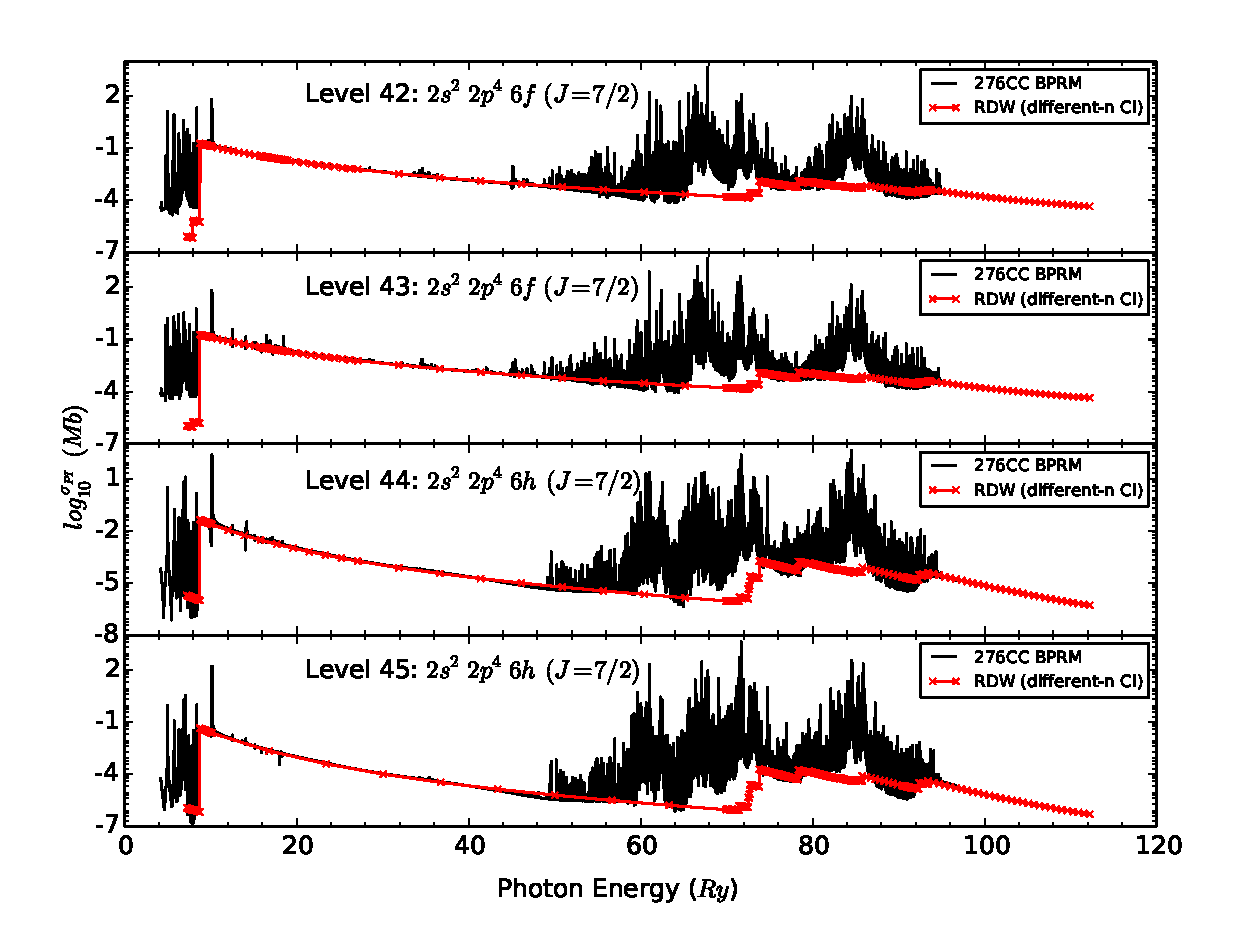
\includegraphics[width=\textwidth]{figures/fe18_mismatch_not_matter.eps}
	\caption{\ion{Fe}{xviii}: The photoionization cross section of levels 42 - 45 as shown in table \ref{table_7_1_44} for both BPRM and RDW. }
	\label{fig_7_1_44_not_matter}
\end{figure}

%======= Figure mismatch_not_matter_tail_other
\begin{figure}
	\centering
	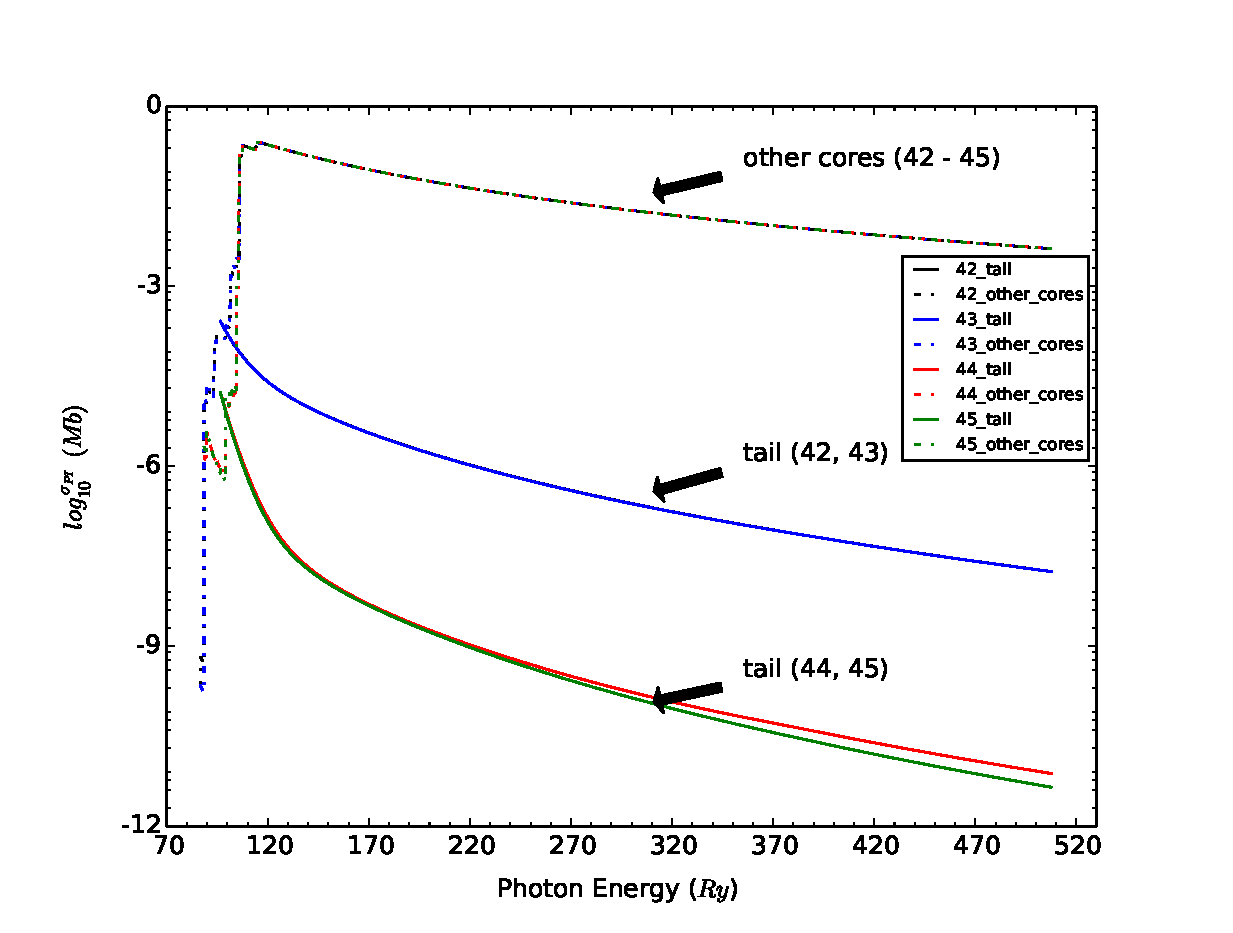
\includegraphics[width=.9\textwidth]{figures/fe18_mismatch_not_matter_tail_other.eps}
	\caption{\ion{Fe}{xviii}: The tail and the contribution from other core configurations of levels 42 - 45 as shown in table \ref{table_7_1_44} for both BPRM and RDW. }
	\label{fig_7_1_44_not_matter_tail_other}
\end{figure}

\subsubsection{Other Bound Levels}
In RDW, we consider all the bound state levels with $n\leq10$, so we collect all such levels that are not included in BPRM calculation, and calculate the photionization cross section due to all core configurations, i.e. the core configurations included in the BPRM calculation and the other ones displayed in section \ref{section_other_targets}, with different-n-complex configuration interaction. For \ion{Fe}{xvii}, there are extra 123 bound levels, while for \ion{Fe}{xviii} there are extra 428 bound levels, so it ends up with 587 bound levels in total for \ion{Fe}{xvii} and 1591 for \ion{Fe}{xviii}. To do a sanity check on the data, we show the photoionization cross section of two levels for each iron ion (see figure \ref{figure_other_levels}) and their energies are listed in table \ref{table_other_levels}. Since there is a big energy gap between $n=2$ and $n=3$ core configurations, the photoionization cross section should decrease smoothly without edges rising up predominantly just as in many figures shown in previous sections, and in figure \ref{figure_other_levels} we can observe such feature for all four levels. In the $n=3$ and $n=4$ core configurations energy region, the transitions are very likely dominated by the different-n-complex configuration interaction, creating many edges followed by a very fast descreasing tail, which is seen in figure \ref{figure_other_levels}. But if the bound level has configuration with the outer electron in $M-,~N-$shell, there will be a big jump in the photoionization cross section. For example, in each top panel of figures \ref{fe17_bprm_fac}, \ref{fe18_bprm_fac} and \ref{figure_fe17_bound_mix}, there is a big jump in the background of photoionization cross section, and RDW does an excellent job in reproducing it. As shown in chapter \ref{chap_pec_l_edge} these jumps are from the  PEC-L-Edge transitions (see table \ref{table_n3_n4_jumps}). In the higher energy region around $100~Ry$, all of the four levels have big jumps due to transitions shown in table \ref{table_n5_n6_jumps}. 

%======== Table other bound levels
\begin{table}
	\centering
	\caption{Listed are four of the bound levels found in the topup calculation and their photoionization cross section is shown in figure \ref{figure_other_levels}. Note: the energy is $z$-scaled ($z=17$ for \ion{Fe}{xvii} and 18 for \ion{Fe}{xviii}), and in unit of $10^{-3} Ry$.}
	\begin{tabular} { | c | c |}
		\hline
		Level & Energy \\
		\hline
		$2s^2 2p^5 10k~(J=8)$ & -6.7798\\
		$2s 2p^65f ~(J=2)$ & -5.8754\\
		$2s 2p^5 6g~(J=11/2)$ & -1.5446\\
		$2s 2p^5 6p~(J=5/2)$ & -1.2772\\
		\hline	  								   
	\end{tabular}
	\label{table_other_levels}
\end{table}

%======= Figure other levels
\begin{figure}
	\centering
	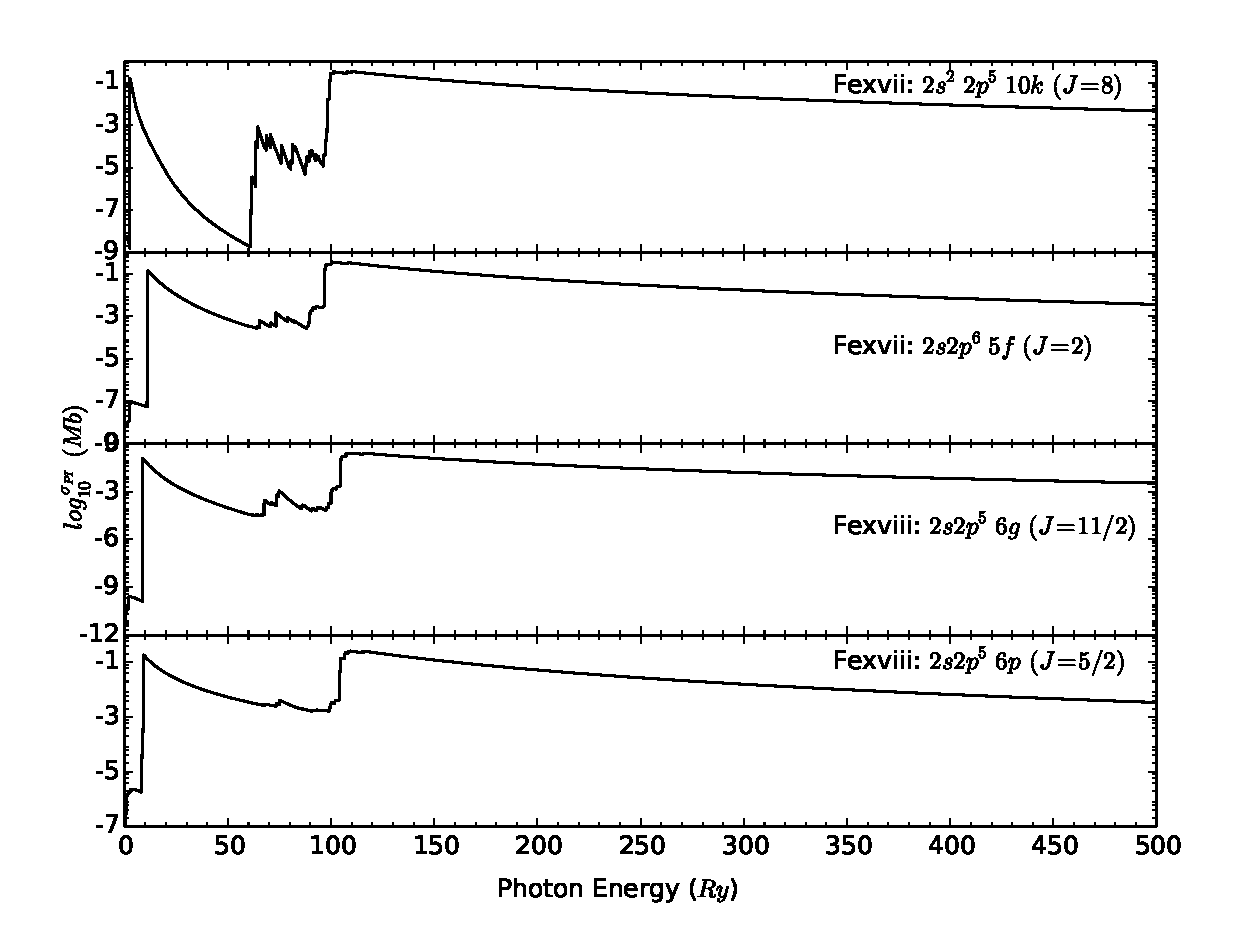
\includegraphics[width=.9\textwidth]{figures/other_levels.eps}
	\caption{Among the other bound levels, 2 of them for both \ion{Fe}{xvii} and \ion{Fe}{xviii} are shown. The configurations and $J$ values are provided. }
	\label{figure_other_levels}
\end{figure}

%======== Table n3 n4 jumps
\begin{table}
	\centering
	\caption{Listed are the main transitions that cause the jump of the background of photoionization cross section as shown in figures \ref{fe17_bprm_fac}, \ref{fe18_bprm_fac} and \ref{figure_fe17_bound_mix}.}
	\begin{tabular} { | c | c |}
		\hline
		Level & Final Configurations \\
		\hline
		$2s^2 2p^5 4d~(J=2)$ & $2s^2 2p^4 4d$, $2s 2p^5 4d$\\
		$2s^2 2p^4 4d~(J=5/2)$ & $2s^2 2p^3 4d$\\
		$2s^2 2p^5 3p~(J=0)$ & $2s^2 2p^4 3p$, $2s 2p^5 3p$\\
		\hline	  								   
	\end{tabular}
	\label{table_n3_n4_jumps}
\end{table}

%======== Table n5 n6 jumps
\begin{table}
	\centering
	\caption{Listed are the main transitions that cause the jump for levels with $n=5,~6,~10$, as shown in figure \ref{figure_other_levels}.}
	\begin{tabular} { | c | c |}
		\hline
		Level & Final Configurations \\
		\hline
		$2s^2 2p^5 10k~(J=8)$ & $2s^2 2p^4 10k$, $2s 2p^5 10k$\\
		$2s 2p^6 5f~(J=2)$ & $2s 2p^5 5f$, $2p^6 5f$\\
		$2s 2p^5 6g~(J=11/2)$ & $2s 2p^4 6g$, $2p^5 6g$\\
		$2s 2p^5 6p~(J=5/2)$ & $2s 2p^4 6p$, $2p^5 6p$\\
		\hline	  								   
	\end{tabular}
	\label{table_n5_n6_jumps}
\end{table}

\subsection{Bound - Bound} \label{section_bound_bound}
To top up the bound-bound oscillator strength, we divide it into two parts. One is from bound states to pure bound states. We calculate all the possible transitions, and only collect the ones that are not calculated in BPRM calculation. The other part is from bound states to quasi-bound states, i.e. doubly excited states. BPRM calculation  treats direct photionization and autoionization as a single quantum-mechanical process \citep{config_2003}, and in section \ref{section_bf}, direct photoionization is discussed, so to simulate the autoionization process, we calculate the oscillator strength from bound to doubly excited states, which is shown to reproduce the resonances very well \citep{ah_1997}. We consider the bound-quasi-bound transitions that excite an electron from $L$-shell to a higher one, forming a doubly excited configuration that can not be formed by combining a core configuration used in BPRM calculation with another electron.

%======= Table bound-bound fe17
\begin{table}
	\centering
	\caption{\ion{Fe}{xvii}: Bound-bound transitions included in the top up calculation. Note: $\ell$, $\ell'$ can be any subshell in each corresponding shell.}
	\label{table_fe17_bound_bound}
	\begin{tabular}{|c||c|c|}
		\hline
		Ion & Initial configurations & Final configurations \\
		\hline
		\multirow{19}{*}{\ion{Fe}{xvii}} & \multicolumn{2}{|c|}{Bound - Pure-Bound ($S+P=7$, $n \leq 10$)} \\
		\cline{2-3}
		& $2s^2 2p^6$ & $2s^S 2p^P n\ell$ ($n\geq3$) \\
		
		&$2s^S 2p^P 3\ell$ & $2s^S 2p^P n\ell$ ($n\geq3$) \\
		
		&$2s^S 2p^P 4\ell$ & $2s^S 2p^P n\ell$ ($n\geq4$) \\
		
		&$2s^S 2p^P 5\ell$ & $2s^S 2p^P n\ell$ ($n\geq5$) \\
		
		&$2s^S 2p^P 6\ell$ & $2s^S 2p^P n\ell$ ($n\geq6$) \\
		
		&$2s^S 2p^P 7\ell$ & $2s^S 2p^P n\ell$ ($n\geq7$) \\
		
		&$2s^S 2p^P 8\ell$ & $2s^S 2p^P n\ell$ ($n\geq8$) \\
		
		&$2s^S 2p^P 9\ell$ & $2s^S 2p^P n\ell$ ($n\geq9$) \\
		
		&$2s^S 2p^P 10\ell$ & $2s^S 2p^P n\ell$ ($n\geq10$) \\
		\cline{2-3}
		& \multicolumn{2}{|c|}{Bound - Quasi-Bound ($S+P=7$, $S'+P'=6$, $n \leq 7$)} \\
		\cline{2-3}
		& \multirow{3}{*} {$2s^S 2p^P 4\ell$} & $2p^6 4\ell n\ell'$ ($n\geq4$)\\
		& & $2s^2 2p^4 4f^2$, $2s^2 2p^4 4f n\ell$ ($n\geq5$) \\
		& & $2s 2p^5 4f^2$, $2s 2p^5 4f n\ell$ ($n\geq5$) \\
		\cline{3-3}
		& \multirow{2}{*} {$2s^S 2p^P 5\ell$} & $2p^6 4\ell 5\ell'$, $2s^2 2p^4 4f 5\ell$, $2s 2p^5 4f 5\ell$\\
		& & $2s^{S'} 2p^{P'} 5\ell n\ell'$ ($n\geq5$) \\
		\cline{3-3}	
		& \multirow{3}{*} {$2s^S 2p^P 6\ell$} & $2p^6 4\ell 6\ell'$, $2s^2 2p^4 4f 6\ell$, $2s 2p^5 4f 6\ell$\\
		& & $2s^{S'} 2p^{P'} 5\ell 6\ell'$\\
		& & $2s^{S'} 2p^{P'} 6\ell n\ell'$ ($n\geq6$)\\
		\cline{3-3}	
		& \multirow{2}{*} {$2s^S 2p^P 7\ell$} & $2p^6 4\ell 7\ell'$, $2s^2 2p^4 4f 7\ell$, $2s 2p^5 4f 7\ell$\\
		& & $2s^{S'} 2p^{P'} n\ell 7\ell'$ ($n\geq5$)\\ 							
		\hline
	\end{tabular}
\end{table}

%======= Table bound-bound fe18
\begin{table}
	\centering
	\caption{\ion{Fe}{xviii}: Bound-bound transitions included in the top up calculation. Note: $\ell$, $\ell'$ can be any subshell in each corresponding shell.}
	\label{table_fe18_bound_bound}
	\begin{tabular}{|c||c|c|}
		\hline
		Ion & Initial configurations & Final configurations \\
		\hline
		\multirow{19}{*}{\ion{Fe}{xviii}} & \multicolumn{2}{|c|}{Bound - Pure-Bound ($S+P=6$, $n \leq 10$)} \\
		\cline{2-3}
		& $2s^S 2p^P 2\ell$ & $2s^S 2p^P n\ell$ ($n\geq2$) \\
		
		&$2s^S 2p^P 3\ell$ & $2s^S 2p^P n\ell$ ($n\geq3$) \\
		
		&$2s^S 2p^P 4\ell$ & $2s^S 2p^P n\ell$ ($n\geq4$) \\
		
		&$2s^S 2p^P 5\ell$ & $2s^S 2p^P n\ell$ ($n\geq5$) \\
		
		&$2s^S 2p^P 6\ell$ & $2s^S 2p^P n\ell$ ($n\geq6$) \\
		
		&$2s^S 2p^P 7\ell$ & $2s^S 2p^P n\ell$ ($n\geq7$) \\
		
		&$2s^S 2p^P 8\ell$ & $2s^S 2p^P n\ell$ ($n\geq8$) \\
		
		&$2s^S 2p^P 9\ell$ & $2s^S 2p^P n\ell$ ($n\geq9$) \\
		
		&$2s^S 2p^P 10\ell$ & $2s^S 2p^P n\ell$ ($n\geq10$) \\
		\cline{2-3}
		& \multicolumn{2}{|c|}{Bound - Quasi-Bound ($S+P=6$, $S'+P' = 5$, $n \leq 7$)} \\
		\cline{2-3}
		& $2s^S 2p^P 3\ell$ & $2p^5 3\ell n\ell'$ ($n\geq 3$) \\
		\cline{3-3}
		& \multirow{3}{*} {$2s^S 2p^P 4\ell$} & $2s 2p^4 4\ell n\ell'$ ($n\geq4$)\\
		& & $2p^5 4\ell n\ell'$ ($n\geq3$) \\
		& & $2s^2 2p^3 4f^2$, $2s^2 2p^3 4f n\ell$ ($n\geq5$) \\
		\cline{3-3}
		& \multirow{4}{*} {$2s^S 2p^P 5\ell$} & $2s^2 2p^3 4f 5\ell$\\
		& & $2p^5 n\ell 5\ell' ($n = 3, 4$)$ \\
		& & $2s 2p^4 4\ell 5\ell'$ \\
		& & $2s^{S'} 2p^{P'} 5\ell n\ell'$  ($n \geq 5$)\\
		\cline{3-3}	
		& \multirow{4}{*} {$2s^S 2p^P 6\ell$} & $2s^2 2p^3 4f 6\ell$\\
		& & $2p^5 n\ell 6\ell' ($n = 3, 4$)$ \\
		& & $2s 2p^4 4\ell 6\ell'$ \\
		& & $2s^{S'} 2p^{P'} n\ell 6\ell'$  ($n \geq 5$)\\
		\cline{3-3}	
		& \multirow{4}{*} {$2s^S 2p^P 7\ell$} & $2s^2 2p^3 4f 7\ell$\\
		& & $2p^5 n\ell 7\ell' ($n = 3, 4$)$ \\
		& & $2s 2p^4 4\ell 7\ell'$ \\
		& & $2s^{S'} 2p^{P'} n\ell 7\ell'$  ($n \geq 5$)\\
		\hline
	\end{tabular}
\end{table}

\subsubsection{Bound - Pure-Bound}
In RDW calculation, we consider the bound configurations with principle quantum number up to 10 of the outer electron, and in BPRM calculation, some bound levels are missed out due to large scanning step and the upper scanning limit of the effective quantum number, thus in the bound to pure-bound transitions, we first calculate all the transitions possible between the bound configurations, which can only be formed by $n=2$ core configurations coupled with an outer electron. See the upper parts of tables \ref{table_fe17_bound_bound} and \ref{table_fe18_bound_bound} for \ion{Fe}{xvii} and \ion{Fe}{xviii}, respectively. Since we have obtained the level correspondence in BPRM and RDW through matching process as described in section \ref{section_matching}, we are readily to exclude the transitions between those levels, and keep the remaining bound to pure-bound transitions. There are some transitions between bound levels found in BPRM to quasi-bound levels which are formed by $n=2$ core configurations coupled with an outer electron, and these transitions are treated naturally as resonances in BPRM calculation, so in section \ref{section_bound_quasi_bound}, we do not include those transitions.  And we do not consider transitions between quasi-bound to quasi-bound levels, as quasi-bound means the levels have energy larger than the ground state of the core configurations, so they are essentially ionized and these transitions are unphysical in opacity calculation.

\subsubsection{Bound - Quasi-Bound}
\label{section_bound_quasi_bound}
Like the other parts of the top up calculation, the bound configurations only consider the same-n-complex configuration interaction. But with different-n-complex configuration interaction, there can be more transitions, e.g. from bound configurations $2s^2 2p^5 3\ell$ to quasi-bound configurations $2s^2 2p^4 4\ell 5\ell'$, though at the cost of losing bound level correspondence obtained in level-matching step as the energy is very likely to change, and to collect the energy information needed by the opacity calculation, the quasi-bound levels are readily available but the bound levels very likely have different energy from those that have already been collected in the bound to pure-bound transitions, and in this case maybe we can just neglect those changed energies, and use the previous one, so only quasi-bound level energy should be collected. Since the current data does not include such transitions, it might be another thing one can consider to improve on later, but it is very likely it will have negligible contribution to opacity. In the bound to quasi-bound top up calculation one can consider the transitions to the quasi-bound configurations with principle quantum number as high as interested, and in the current calculation we go up to 7, since the higher n introduces hundreds of thousands of quasi-bound levels, and it is very likely they are negligible compared with the big jump in photoionization cross section. In the following, I will give a detailed clarification on these transitions listed in tables \ref{table_fe17_bound_bound} and \ref{table_fe18_bound_bound}. 

In \ion{Fe}{xvii} 218 CCBPRM calculation, it includes complete $n=2$ core configurations, i.e. $2s^S 2p^P$, which can form possible quasi-bound configuratoins $2s^S 2p^P n\ell$. It also includes complete $n=3$ core configurations, i.e. $2s^{S'} 2p^{P'} 3\ell$ where $S'+P' = 6$, which can form possible quasi-bound configurations $2s^{S'} 2p^{P'} 3\ell n\ell'$ where $3 \leq n \leq 7$. And it includes part of the $n=4$ core configurations, i.e.  $2s^{S'} 2p^{P'} 4\ell$ where $S' = 1-2, ~\ell = 0-2$, which can form quasi-bound configurations $2s^{S'} 2p^{P'} 4\ell 4\ell'$, $2s^{S'} 2p^{P'} 4\ell n\ell'$ where $5 \leq n \leq 7$. Thus the bound levels in configurations $2s^2 2p^6$ and $2s^S 2p^P 3\ell$ are treated completely. For bound configurations $2s^S 2p^P 4\ell$, the resonances can be formed by transitions to possible quasi-bound configurations are $2s^S 2p^P n\ell$, $2s^{S'} 2p^{P'} 3\ell 4\ell'$, $2s^{S'} 2p^{P'} 4\ell 4\ell'$, $2s^{S'} 2p^{P'} 4\ell 5\ell'$, $2s^{S'} 2p^{P'} 4\ell 6\ell'$ and $2s^{S'} 2p^{P'} 4\ell 7\ell'$, of which the first two have already been included completely in BPRM and part of the rest are also included, leaving out $2p^6 4\ell n\ell'~(4 \leq n \leq 7)$, $2s^2 2p^4 4f^2$, $2s 2p^5 4f^2$, $2s^2 2p^4 4f n\ell$ and  $2s 2p^5 4f n\ell~(5 \leq n \leq 7)$ unconsidered. So in the top up calculation, we consider the transitions from  $2s^S 2p^P 4\ell$ to the quasi-bound configurations that are missed out. For the bound levels in configurations  $2s^S 2p^P 5\ell$, the possible quasi-bound configurations are  $2s^S 2p^P n\ell$,  $2s^{S'} 2p^{P'} 3\ell 5\ell'$, $2s^{S'} 2p^{P'} 4\ell 5\ell'$,  $2s^{S'} 2p^{P'} 5\ell n\ell'$ ($5 \leq n \leq 7$), so the missing configurations in BPRM are $2p^6 4\ell 5\ell'$, $2s^2 2p^4 4f 5\ell$, $2s 2p^5 4f 5\ell$, $2s^{S'} 2p^{P'} 5\ell n\ell'$ ($5 \leq n \leq 7$). As for bound levels in $2s^S 2p^P 6\ell$ and $2s^S 2p^P 7\ell$, it is very similar to $2s^S 2p^P 5\ell$, and the missing quasi-bound configurations are listed as shown in table \ref{table_fe17_bound_bound}.

In \ion{Fe}{xviii} 276 CCBPRM calculation, it includes complete $n=2$ core configurations, i.e. $2s^S  2p^P$, so it can form possible quasi-bound configurations $2s^S  2p^P n\ell$. It includes part of the $n=3$ core configurations, i.e. $2s^2 2p^3 3\ell$ and $2s 2p^4 3\ell$, and they can form possible quasi-bound configurations $2s^2 2p^3 3\ell n\ell'$ and $2s 2p^4 3\ell n\ell'$ ($3 \leq n \leq 6$). It also includes part of the $n=4$ core configurations, i.e. $2s^2 2p^3 4\ell$ ($\ell \leq 2$), and they can form quasi-bound configurations $2s^2 2p^3 4\ell n\ell'$ ($4 \leq n \leq 7$). So like \ion{Fe}{xvii}, bound levels in $2s^S 2p^P 2\ell$ are treated completely. For levels in bound configurations $2s^S 2p^P 3\ell$, the resonances can be due to transitions to quasi-bound configurations $2s^S 2p^P n\ell$ and  $2s^{S'} 2p^{P'} 3\ell n\ell'$ ($3 \leq n \leq 7$), so the missing quasi-bound configurations are $2p^5 3\ell n\ell'$ ($3 \leq n \leq 7$). For the bound levels in configuratoins $2s^S 2p^P 4\ell$, the possible quasi-bound configurations formed can be $2s^S 2p^P n\ell$, $2s^{S'} 2p^{P'} 3\ell 4\ell'$ and $2s^{S'} 2p^{P'} 4\ell n\ell'$ ($4 \leq n \leq 7$), so the missing configurations are $2p^5 3\ell 4\ell'$,  $2p^5 4\ell n\ell'$ ($4 \leq n \leq 7$), $2s 2p^4 4\ell n\ell'$ ($4 \leq n \leq 7$), $2s^2 2p^3 4f^2$ and $2s^2 2p^3 4f n\ell$ ($n = 5, ~6,~7$).  For the bound levels in configuratoins $2s^S 2p^P 5\ell$, the possible quasi-bound configurations formed can be $2s^S 2p^P n\ell$, $2s^{S'} 2p^{P'} 3\ell 5\ell'$, $2s^{S'} 2p^{P'} 4\ell 5\ell'$ and  $2s^{S'} 2p^{P'} 5\ell n\ell'$~($5 \leq n \leq 7$), so the missing configurations are $2p^5 3\ell 5\ell'$, $2s^2 2p^3 4f 5\ell$, $2s 2p^4 4\ell 5\ell'$, $2p^5 4\ell 5\ell'$ and $2s^{S'} 2p^{P'} 5\ell n\ell'$~($5 \leq n \leq 7$). For bound levels in $2s^S 2p^P 6\ell$ and  $2s^S 2p^P 7\ell$, it is very similar to $2s^S 2p^P 5\ell$, and the missing quasi-bound configurations are listed as shown in table \ref{table_fe18_bound_bound}.

\section{Conclusion}
Relativistic distorted wave calculation is performed for \ion{Fe}{xvii} and \ion{Fe}{xviii} to top-up the 218 and 276 CCBPRM calculation, respectively. Bound state levels are matched between BPRM and RDW calculation by comparing quantumn numbers $J$, $\pi$, energy, and photoionization cross section. With such level correspondance, the photoionization cross section of BPRM calculation in the higher energy region is extended using RDW data, and contribution from other core configurations up to $n=10$ is added. Other bound state levels are also included with photoionization cross section due to all the core configurations up to $n=10$. Including core configurations up to $n=10$ is crucial in that it ensures the PEC-L-Edge transitions for each bound state level, thus the jump showing up at around $100~Ry$ ensures the convergence of the photoionization cross section. Oscillator strength is also topped up, with contribution from bound-pure-bound transitions and bound-quasi-bound transitions with outer electron up to $n=7$. 
The effects of configuration interaction on photoionization cross section are discussed, including same-n-complex and different-n-complex, showing its significant role in reproducing the background of BPRM using RDW. Different-n-complex configuration interaction is important in the region before the PEC-L-Edge transitions kick in, and in some levels shown in figure \ref{figure_other_levels}, it changes the background dramatically in a few tens of Rydbergs. 

\begin{appendices}
	\include{app_2/bprm_code}
	\chapter{Top Up Procedure and Analysis} \label{app_topup_procedure_analy}

\section{Overview of the Top Up Code}
As described in chapter \ref{chap_topup}, the top up calculation is done by firstly establishing correct level correpondance between BPRM and RDW calculation, and this ensures extending the correct tail, adding the contribution from the correct other target configurations, and including the correct unincluded bound levels. In the flowchart \ref{fig_topup_flowchart}, as you can see, the main procedure is divided into two parts, one focues on the matching step, and the other on the top up step. In the matching step, which starts in directory \textbf{\textit{match/}}, we need to firstly finish the RDW calculation with only the core configurations included in BPRM calculation, and the scripts in direcotries \textbf{\textit{bound\_levels\_0/}}, \textbf{\textit{create\_mesh\_1/}} and \textbf{\textit{generate\_PI\_2/}} will extract the bound levels, create energy mesh for each level and generate the photoionization cross section, respectively. Now we are ready to do the matching. Since BPRM code categorizes the bound levels by $2J$ and $\pi$, and these levels are sorted in energy-ascending order, the script in \textbf{\textit{bound\_levels\_0/}} just does this job, and the photoionization cross section are generated in the same order. Thus we can just blindly match the levels in BPRM and RDW calculations by level index and plot the photoionization cross section against each other. Usually we get a roughly good match, and the RDW cross section does reproduce the background of BPRM calculation very well. However, as illustrated in section \ref{section_matching}, due to the energies being closely packed in a small region, these levels can not be distinguished by energy, and we should carefully inspect the matching of the photoionization cross section. Once we decide to match level $m$ in BPRM calculation with level $n$ in RDW calculation, and level $n$ in BPRM with level $m$ in RDW, we put such pairs $m~~n$ and $n~~m$ in each line in file \textbf{\textit{correct\_match\_n4}}, and replot the photoionization cross section. Such iteration is repeated until satisfatory result is achieved. In section \ref{section_matching}, I mentioned a ``fake'' level found in BPRM calculation, and I assigned one level in RDW twice to the two almost the same levels in BPRM. When all levels are matched, the correction to the matching should be stored in folder $correct\_match\_n3$ or $correct\_match\_n4$ with names as $2J\_\pi$. The complete result can be found at \url{https://github.com/zhao1157/PhD-Atomic-Physics/tree/master/fe17_fe18_matched_levels} for both \ion{Fe}{xvii} and \ion{Fe}{xviii}. And these level information, especially the configuration, can be readily extracted. In $ratio\_analysis\_4$, we can utilized the matched levels and categorize them in terms of ratio of BPRM/RDW at the last point. For more details, see section \ref{section_detailed_topup_code}. I also put the bound-bound top up calculation inside $match/$ because of the identified levels in $level\_identification\_3/$. 

Once levels are appropriately matched, we are all set to proceed the top up calculation, i.e. extending the tail, adding the contribution from other core configurations, and including the levels that are missed out. In folder $topup/$, the level matching correction information from $match/$ is needed here. To extend the tail,we need to find the last energy point in each level in BPRM calculation, which decides the starting point at which we need to create new energy mesh, and its lowest ionizaiton threshold, i.e. the absolute value of its energy, which decides the end of the energy mesh, i.e. $500~Ry$ more than the lowest ionization threshold. And this is done in $extract\_bprm\_tail\_n4\_0/$. Then we need to do RDW calculation including the other core configurations only, and extract these new thresholds for each level and sort them in ascending order and find the ones that are beyond the last point in BPRM calculation. The tail energy mesh is created with these new thresholds and 10 points are assigned between adjacent thresholds, and a few hundred of points between the last threshold and the maximum energy point, i.e.  $500~Ry$ more than the lowest ionization threshold which is found in $extract\_bprm\_tail\_n4\_0/$. In \textbf{\textit{generate\_PI\_2/}}, the RRTable should be the one containing only the core configurations included in BPRM. In \textbf{\textit{combine\_tail\_3/}}, these tails are added to BPRM data. Now we are ready to add the contribution from other core configurations to the tailed BPRM data. Obviously we need to use the RRTable including only the other core configurations, and be aware that there are cases where there are no transitions from some levels to these core configurations, so we add nothing. For those levels which do have extra transitions due to these core configurations, we find the lowest threshold for each level and extract the energy mesh from the tailed BPRM data that is larger than the lowest threshold. After the calculation is done, the whole data can be combined in \textbf{\textit{combine\_other\_targets\_3/}}. By far the complete data has been obtained for those levels included in BPRM calculation. 

As stated in chapter \ref{chap_topup}, the bound levels are counted with principle quantum number wihthin 10, so we exclude the levels that have been included in BPRM calculation, and collect the rest. This is done in \textbf{\textit{other\_levels\_2/}}. The complete photoionization cross section is plotted and accessible at \url{https://github.com/zhao1157/PhD-Atomic-Physics/tree/master/fe17_fe18_full_data}. In addition, I also wrote a script that can extract the transition information for one level in \textbf{\textit{extract\_free\_config\_3/}}. To find the transition information for the jumps of all levels, go to \textbf{\textit{extract\_jump\_4/}}.

%===== FLOWCHART
\begin{figure}
	\centering
	\includegraphics[width=1.0\textwidth]{app_1/figures/topup_procedure_flowchart}
	\caption{The architecture of the code that is written for the top up calculation and analysis. It is available in \url{https://github.com/zhao1157/PhD-Atomic-Physics}.}
	\label{fig_topup_flowchart}
\end{figure}

\section{Detailed Description of the Top Up Code}
\label{section_detailed_topup_code}
Since this top up procedure is divided into several parts and in each part there are a few separate scripts needed to be executed, the names of these parts and scripts implicitly tells the relative order of executing them. For example, folders \textbf{\textit{bound\_levels\_0/}}, \textbf{\textit{create\_mesh\_1/}} and \textbf{\textit{generate\_PI\_2/}} have to executed in the order as the last index before `\_' indicates. And the scripts in \textbf{\textit{create\_mesh\_1/}}, i.e. \textbf{\textit{extract\_trans\_awk\_1.sh}}, \textbf{\textit{collect\_thresh\_awk\_2.sh}}, \textbf{\textit{order\_thresh\_awk\_3.sh}}, \textbf{\textit{add\_mini\_diff\_awk\_4.sh}} and  \textbf{\textit{creat\_fine\_mesh\_5.py}}, have to be executed in the order as the index between `\_' and the extension of the file name indicates. The following is a detailed description of the important scripts.

\subsection{\textit{match/}}
\begin{enumerate}
	\item \textbf{\textit{bound\_levels\_0/}}: extract the bound levels that contribute to the photoionization cross section, in terms of $2J$ and $\pi$.
		\begin{itemize}
			\item \textit{extract\_bound\_levels\_0.py}: input the files that contain the energy and RRTable, the number of electrons of the bound configurations, the charge of the core confgurations, and the energy of the ground state of the core configurations in unit of ev. Note it is more accurate to use the energy of the ground state of the core with same-n-complex configuration interaction, though different-n-complex configuration interaction of the core configurations is used to maximally reproduce the background of BPRM calculation. It outputs the levels in energy ascending order for each symmetry $2J\_\pi$, and the negative and positive levels are separated.
		\end{itemize}
		
	\item \textbf{\textit{create\_mesh\_1/}}: create energy mesh for each bound state level. To delineate the edges, 10 points are uniformly assigned between adjacent thresholds.
		\begin{itemize}
			\item \textit{extract\_trans\_awk\_1.sh}: collect the transition information for the levels of interest, i.e. the header line for each transition. Usually we need to create a symlink that points to a file which contains the levels we are interested in, e.g. \colorbox{gray!20} {\textit{ln -s ../bound\_levels\_0/0\_0\_neg bound\_levels\_0}} (see script \textit{run\_JJ\_Pi.sh} in \textbf{\textit{match/}} below).
			\item \textit{collect\_thresh\_awk\_2.sh}:  collect the various thresholds for each level, and output the level index and its thresholds in one single line.
			\item \textit{order\_thresh\_awk\_3.sh}: sort the thresholds for each level in ascending order, and append each level with an energy that is 105 Ry (or another range of your interest) more than the lowest threshold, and remove other thresholds that are the same as one threshold.
			\item \textit{add\_mini\_diff\_awk\_4.sh}: append the smallest difference between adjacent thresholds at the end of each line for each level. This value is useful when creating energy mesh and 10th of it is used as the increment. So in this way we try to delineat the edges of various transitions.
			\item \textit{creat\_fine\_mesh\_5.py}: create an energy mesh for each level, with 10 points in any adjacent shresholds, and 20 points between the last threshold and the maximal energy point.
			\item \textit{test\_same.awk}:  it is called inside of \textit{creat\_fine\_mesh\_5.py} to test the fine mesh whether the adjacent points are the same or not. Usually I do not use it.
			\item \textit{run.sh}: show the order of executing the scripts above. It is usually called in a loop to run these steps.
		\end{itemize}
	
	\item \textbf{\textit{generate\_PI\_2/}}: after mesh being generated, the scripts in this folder calculate the photoionization cross section.
		\begin{itemize}
			\item \textit{fe18\_n3.py}:  load the existing energy binary file and RRTable binary file and interpret and extrapolate the photoionization cross section for each level in the energy mesh created in \textit{create\_mesh\_1/}. In this script, we use \textit{fac.InterpCross()} to output the data for each transition and then to do the summation over all transitions for each level. We can also use \textit{fac.TotalPICross()} to get the summed result, but in many situtations the energy mesh and number of transitions are large which results in the large memory requirement. Thus we abandon it in general.
			\item \textit{add\_awk.sh}: after \textit{fac.InterpCross()} generates the data for all transitions, it reads the data and sums it up in unit of $Mb$.
		\end{itemize}
	
	\item \textit{run\_JJ\_Pi.sh}: after the bound levels are extracted in directory \textbf{\textit{bound\_levels\_0/}}, we are ready to generate the photoionization cross section for each level in each symmetry category $2J\_\pi$.
	
	\item \textbf{\textit{level\_identification\_3/}}: As the levels are sorted in energy-ascending order for each symmetry $2J\_\pi$ just as in BPRM calculation, we are ready to just plot the the photoionization cross section of RDW and BPRM. While checking how well they match, we need to make sure the energy agrees well. In some situations, we need to switch or shift the levels so that they are matched. After finishing matching the levels, we are ready to print out the level information and find out the configuraiton of each level.
		\begin{itemize}
			\item \textit{plot\_n4\_background\_1.py}: plot the photoionization cross section of RDW and BPRM and see how well they match with each other. Correction is needed if they don't agree well by switching or shifting to other reasonable levels. File \textit{correct\_match\_n4} or \textit{correct\_match\_n3}, where n3 or n4 refers to n=3 or n=4 core configuraitons, contains the information of level switching. These numbers represent the LINE NUMBER of the level in \textit{../bound\_levels\_0/2J\_$\pi$\_neg} file, assuming the BPRM levels are also written in a file in the same format. In the script, we need to set the number of levels in the symmetry of interest in BPRM calculation. Usually the number of levels obtained in BPRM calculation is no more than that got from RDW. Required is the number of lines that contain the energies of the core states in the front of each level data set in BPRM calculation.
			\item \textit{level\_identification\_2.py}: in this script, the file that contains the correction in matching step is needed, and variable $level\_JJ\_Pi$ is a dictionary contains $2J\_\pi~:~number\_of\_levels\_in\_BPRM$.
			\item \textit{cat.sh}: a simple script to concatenate the level information into a single file that is needed in 
		\end{itemize}
	
	\item \textbf{\textit{ratio\_analysis\_4/}}: extract the information of the levels whose ratios fall within a range. This script is useful if you want to get a rough idea of how well the calculation of BPRM and RDW agrees with each other at the last point, and what kind of levels do well and not well. The order of the levels written in files \textit{level\_file} and \textit{ratio\_file} has to be the same. Usually it is $0\_0$ ($2J\_\pi$), $0\_1$, $2\_0$, $2\_1$, ..., $16\_0$, $16\_1$ for \ion{Fe}{xvii}, but of course it can vary as long as they are in the same fashion in these two files.
	\begin{itemize}
		\item \textit{ratio\_configurations.py}: it collects the levels whose ratio $<0.5$ in 0, $>=0.5~\&<1.5$ in 1, $>=1.5~\&<2.5$ in 2, etc., the rest of levels in n (in line 8, \colorbox{gray!20}{\textit{ratios = range(n)}}).
	\end{itemize}
	
	\item \textbf{\textit{bb\_5/}}: does the bound-bound top up calculation.
	\begin{itemize}
		\item \textit{create\_e\_file.py}: create e-file needed in opacity calculation. In line 7, variable $ind\_max\_remove$ represents the maximum level index that bound-quasi-bound transitions should be neglected as they are already included in BPRM. In the $fac.Structure()$ part, the bound configurations have to be in front of the other quasi-bound configurations. In line 73, it excludes the transitions that are from the positive-energy levels, the transitions that have already been included in BPRM stgbb, and the ones that have already been included in bound-free, i.e. resonances due to $n=2$ core configurations coupled with an outer electron. In list $file\_en\_454\_rest$, the first file has to be energy file, followed by the transition files. These transition files have to share the same energy file, otherwise when reading different transition files, levels will be messed up.
		\item \textit{create\_f\_file.py}: creates f-file needed in opacity calculation. The same variable settings as in file \textit{create\_e\_file.py}.
	\end{itemize}
\end{enumerate}

\subsection{\textit{topup/}}
\begin{enumerate}
	\item \textbf{\textit{extract\_bprm\_tail\_n4\_0/}}
		\begin{itemize}
			\item \textit{extract\_bprm\_0.py}: used to extract the threshold and last point for each level in bprm data for tail-processing. The threshold is used to determine the highest energy point, i.e. $500~Ry$ more than the threshold. The last point is used to compare with various thresholds in order to determine the thresholds that are beyond this point.
		\end{itemize}
	
	\item \textbf{\textit{tail\_other\_targets\_1/0-16/}}
		\begin{enumerate}
			\item \textbf{\textit{bound\_levels\_0/}}: only consider the transitions to other core configurations as we want to extract the thresholds due to them, so that the energy mesh can be created appropriately.
				\begin{itemize}
					\item \textit{extract\_bound\_levels\_0.py}: the same as the one in \textbf{\textit{match/bound\_levels\_0/}}.
				\end{itemize}
		
			\item \textbf{\textit{create\_mesh\_1/}}: the filenames of these scripts are the same as those in 
			\textbf{\textit{match/create\_mesh\_1/}}, but the content can be drastically different.
				\begin{itemize}
					\item \textit{extract\_trans\_awk\_1.sh}: the same as those in \textbf{\textit{match/create\_mesh\_1/}}.
					\item \textit{collect\_thresh\_awk\_2.sh}: the same as those in \textbf{\textit{match/create\_mesh\_1/}}.					
					\item \textit{order\_thresh\_awk\_3.sh}: compared with the one in \textbf{\textit{match/create\_mesh\_1/}}, line 19 is commented out in the current version, because the lowest threshold for each level is stored in \textbf{\textit{extract\_bprm\_tail\_n4\_0/}}.					
					\item \textit{add\_mini\_diff\_awk\_4.sh}: the same as those in \textbf{\textit{match/create\_mesh\_1/}}.			
					\item \textit{creat\_fine\_mesh\_5.py}: due to the correction in matching step, we first reorder the levels obtained from \textit{add\_mini\_diff\_awk\_4.sh}, and then determine how to create the energy mesh. If all the thresholds are within the last point of BPRM calculation, then we simply assign 400 points between the last point and the point which is 500 Ry above the threshold obtained in \textbf{\textit{extract\_bprm\_tail\_n4\_0/}}. Otherwise, we find the threshold that just starts to become larger than the last point, and assign 10 points between the last point and that threshold, and also 10 points between the following thresholds, and 300 points between the last threshold and the point which is $500~Ry$ above the threshold obtained in \textbf{\textit{extract\_bprm\_tail\_n4\_0/}}.					
					\item \textit{test\_same.awk}: the same as those in \textbf{\textit{match/create\_mesh\_1/}}.					
					\item \textit{run.sh}: it is slightly different from the one in \textbf{\textit{match/create\_mesh\_1/}}, in that \textit{creat\_fine\_mesh\_5.py} needs to read some input parameters, i.e. $2J$ and $\pi$.					
				\end{itemize}
			
			\item \textbf{\textit{generate\_PI\_2/}}: since we are extending the tail, which is due to the core configuraitons that are included BPRM calculation, only these core configuraitons are considered.
				\begin{itemize}
						\item \textit{fe18\_n3.py}: the same as those in \textbf{\textit{match/generate\_PI\_2/}}.		
						\item \textit{add\_awk.sh}: the same as those in \textbf{\textit{match/generate\_PI\_2/}}.
				\end{itemize}
			\item \textbf{\textit{combine\_tail\_3/}}: attach the RDW tail to BPRM.
				\begin{itemize}
					\item \textit{combine\_tail.py}: since the levels have already been corrected, we are ready to just concatenate the tail to BPRM data. Note, in this script, we can get the ratio of BPRM/RDW at the last point, which can give us a rough idea of how these two calculation compare with each other. Through this ratio, we can find the levels that are doing well and not well using script in \textbf{\textit{match/ratio\_analysis\_4/}}. To activate this option, uncomment out line 34, and comment out line 35.
					\item \textit{cat.sh}: simply to concatenate $2J\_\pi\_ratio$ files into one file ratio, which is needed in \textbf{\textit{match/ratio\_analysis\_4/}}.
				\end{itemize}
			\item \textbf{\textit{other\_targets\_4/}}: We are going to add the contribution from other core configurations to the tailed-BPRM data. Before proceeding, we need to create a symlink in this directory to \textbf{\textit{../bound\_levels\_0/}}, i.e. \colorbox{gray!20}{\textit{ln -s ../bound\_levels\_0/}}, because the bound level information is the same.
				\begin{enumerate}
					\item \textbf{\textit{create\_mesh\_1/}}: extract the energy mesh for each level.
						\begin{itemize}
							\item \textit{extract\_trans\_awk\_1.sh}: the same as those in \textbf{\textit{match/create\_mesh\_1/}}.
							\item \textit{collect\_thresh\_awk\_2.sh}: the same as those in \textbf{\textit{match/create\_mesh\_1/}}.		
							\item \textit{order\_thresh\_awk\_3.sh}: comment out line 19, as the mesh has already been created, now we just need to find the lowest threshold, and extract the energy mesh.
							\item \textit{extract\_mesh\_4.py}: we take note of the energy index at which the contribution from other core configurations starts to kick in in each level and the rest of the energy points are the mesh we need. And there are cases where there are no transitions to these core configurations, so we denote it as \textit{skip}. These information will be needed when adding the extra contribution to the tailed-BPRM data.
							\item \textit{run.sh}: run the first three scripts.
						\end{itemize}
					\item \textbf{\textit{generate\_PI\_2/}}: calculate the photoionization cross section.
						\begin{itemize}
							\item \textit{fe18\_n3.py}: the same as those in \textbf{\textit{match/generate\_PI\_2/}}.		
							\item \textit{add\_awk.sh}: the same as those in \textbf{\textit{match/generate\_PI\_2/}}.
						\end{itemize}
					\item \textbf{\textit{combine\_other\_targets\_3/}}
						\begin{itemize}
						\item \textit{combine\_other\_targets.py}: combine the tailed-BPRM data with those in \textbf{\textit{generate\_PI\_2/}}.	
						\item \textit{cat.sh}: simply concatenate the these data into one file.
					\end{itemize}
				\end{enumerate}
		\end{enumerate}
	\item \textbf{\textit{other\_levels\_2/}}: We are going to collect all the other bound levels and calculate the photoionization cross section due to all the core configurations included in BPRM calculation and the above top up calculation.
		\begin{enumerate}
			\item \textbf{\textit{bound\_levels\_0/}}: 
				\begin{itemize}
					\item \textit{extract\_bound\_levels\_0.py}: the same as those in \textbf{\textit{match/bound\_levels\_0/}}.		
					\item \textit{extract\_other\_levels\_1.py}:extract all the other bound levels that are not included in BPRM calculation. Note the correction in matching is needed, and variable \textit{sym\_level} is a dictionary containing $2J\_\pi~:~number\_of\_levels\_in\_BPRM$.
					\item \textit{create\_e\_file.py}: create the e-file needed in opacity calculation for these bound levels. Variable $ind\_base$ is the number of bound levels included in BPRM calculation, so the unincluded bound levels are indexed based on that number.
				\end{itemize}
			\item \textbf{\textit{create\_mesh\_1/}}: 
				\begin{itemize}
					\item \textit{extract\_trans\_awk\_1.sh}: the same as those in \textbf{\textit{match/create\_mesh\_1/}}.
					\item \textit{collect\_thresh\_awk\_2.sh}: the same as those in \textbf{\textit{match/create\_mesh\_1/}}.
					\item \textit{order\_thresh\_awk\_3.sh}: the same as those in \textbf{\textit{match/create\_mesh\_1/}}.
					\item \textit{add\_mini\_diff\_awk\_4.sh}: the same as those in \textbf{\textit{match/create\_mesh\_1/}}.	
					\item \textit{creat\_fine\_mesh\_5.py}: compared with the one in \textbf{\textit{match/create\_mesh\_1/}}, it differs in the way of assigning the points between adjacent thresholds. If the difference is within $10~ev$, then 10 points, othewise 20.
					\item \textit{split.sh}: split the energy mesh into a few files, each of which contains 1000 levels. This might be helpful when there are so many levels and the number of transitions is huge, so we can split the calculation in a few chunks and run them simultaneously. 1000 can be changed to other values.
					\item \textit{test\_same.awk}: the same as those in \textbf{\textit{match/create\_mesh\_1/}}.
					\item \textit{run.sh}: run the above scripts.	
				\end{itemize}
			\item \textbf{\textit{generate\_PI\_2/}}:
				\begin{itemize}
					\item \textit{fe18\_n4.py}: it is essentially the same as the one in \textbf{\textit{match/generate\_PI\_2/}}, but it differs a bit in that it reads an input and the file path changes a bit.
					\item \textit{add\_awk.sh}: the same as the one in \textbf{\textit{match/generate\_PI\_2/}}.
					\item \textit{create\_run\_0.sh}: creates PBS jobs for computation of differents chunks. 1000 should be changed if it is changed in \textit{create\_mesh\_1/split.sh}.
					\item \textit{check\_zero\_1.py}: remove the entries that has photoionization cross section of 0.
					\item \textit{combine\_head\_data\_2.py}: it needs a file called head that contains the same energy of the core configurations as in BPRM calculation, and a file containing the level information, i.e. \colorbox{gray!20} {ln -s ../bound\_levels\_0/neg levels}.
				\end{itemize}
			\item \textbf{\textit{extract\_free\_config\_3/}}:
				\begin{itemize}
					\item \textit{extract\_free\_config.py}:  it finds the transitions that contribute most of the photoionization cross section for a level in a given range ($en\_start$, $en\_end$). $exp\_pi$ is a list that contains the exponents of the photoionization cross section.
				\end{itemize}
			\item \textbf{\textit{extract\_jump\_4/}}: to analysis the PEC\_L\_Edge transitions.
				\begin{itemize}
					\item \textit{extract\_jump\_start\_end\_1.py}: extract the PEC\_L\_Edge main transitions for each level. The output file is named as $level\_exp$, e.g. $100\_+01$, in which written are the transitions from level 100 with a magnitude of $10^{+01}$ at the first default energy point.
					\item \textit{extract\_jump\_start\_end\_2.py}: print out the level index, the first and last thresholds for all levels, which are grouped as the principle quantum number of the outer electron.
					\item \textit{extract\_jump\_start\_end\_3.py}: extract the photoionization cross section near the ``last'' threhold and $500~Ry$.
				\end{itemize}
			
		\end{enumerate}
\end{enumerate}


\end{appendices}	
\backmatter	

%\bibliography{references} %uncomment this when using separated bibliography file.
%\bibliographystyle{unsrt}  %uncomment this for numbering of references.
%include the bibliography in the main .tex file to avoid the failure of citing authors' names.
\begin {thebibliography} {}
%============== A
\bibitem[Ahmad et al.(2002)]{neutrino_sno} Ahmad, Q.R., Allen, R.C. et al. 2002, Phys. Rev. Lett., 89, 011301
\bibitem[Antia and Chitre(1997)]{solar_neutrino_1} Antia, H.M., and Chitre, S.M. 1997, Mon. Not. R. Astron. Soc., 289, L1
\bibitem[Antia and Basu(2005)]{ssm_op05_2} Antia, H.M., and Basu, S. 2005, Astrophys. J., 620, L129
\bibitem[Asplund et al.(1999)]{3d_nonlte_2} Asplund, M., Nordlund, \AA., and Trampedach, R. 1999, ASP Conf. Ser., 173, 221
\bibitem[Asplund et al.(2000)]{3d_nonlte_1} Asplund, M., Nordlund, \AA., and Trampedach, R., et al. 1999, Astron. Astrophys., 359, 729
\bibitem[Asplund et al.(2004)]{ags_05_3} Asplund, M., Grevesse, N., Sauval, A.J., et al. 2004, Astron. Astrophys. 417, 751
\bibitem[Asplund et al.(2005)]{ags_05_4} Asplund, M., Grevesse, N., Sauval, A.J. 2005, ASPCS 336, 25
\bibitem[Asplund et al.(2009)]{agss09} Asplund, M., Grevesse, N., et al. 2009, Annu. Rev. Astron. Astrophys. 47, 481

%============= B
\bibitem [Badnell et al.(2005)] {config_2005} Badnell, N.R., Bautista, M. A., Butler, K., et al. 2005, MNRAS, 360, 458

\bibitem [Badnell \& Seaton(2003)] {config_2003} Badnell, N. R., \& Seaton, M. J. 2003, J. Phys. B -- At. Mol. Opt. Phys., 36, 4367

\bibitem[Bahcall et al.(1982)]{ssm_1} Bahcall, J.N., Huebner, W.F., Lubow, S.H., Parkerk, P.D., and Ulrich, R.K. 1982, Rev. Mod. Phys., 54, 767

\bibitem[Bahcall et al.(1988)]{ssm_2} Bahcall, J.N., and Ulrich, R.K. 1988, Rev. Mod. Phys., 60, 297

\bibitem[Bahcall et al.(1995)]{ssm_3} Bahcall, J.N., and Pinsonneault, M.H. 1995, Rev. Mod. Phys., 67, 781

\bibitem[Bahcall and Pinsonneault(1997)]{solar_neutrino_2} Bahcall, J.N., and Pinsonneault. M.H. 1997, Phy. Rev. Lett. 78, 171

\bibitem[Badcall(2003)]{ssm_history} Badcall, J.N. 2003, Nuc. Phys. B Proc. Suppl., 118, 77

\bibitem[Bahcall et al.(2004)]{convec_1} Bahcall, J.N., Serenelli, A.M., and Pinsonneault, M. 2004, Astrophys. J., 614, 464

\bibitem[Bahcall and Pinsonneault(2004)]{convec_2} Bahcall, J.N., and Pinsonneault, M.H. 2004,  Phys. Rev. Lett., 92, 121301

\bibitem[Bahcall et al.(2005)]{ssm_98_05} Bahcall, J.N., Basu, S., Pinsonneault, M., et al. 2005, Astrophys. J., 618, 1049

\bibitem[Bahcall et al.(2005)]{ssm_op05_1} Bahcall, J.N., Serenelli, A.M., and Basu, S. 2005, Astrophys. J., 621, L85

\bibitem[Bailey et al.(2007)]{z_150ev_1} Bailey, J.E., Rochau, G.A., Iglesias, C.A., et al. 2007, Phys. Rev. Lett., 99, 265002

\bibitem[Bailey et al.(2008)]{z_150ev_2} Bailey, J.E., Rochau, G.A., Mancini, R.C., et al. 2008, Rev. Sci. Instrum. 79, 113104

\bibitem[Bailey et al.(2009)]{opacity_exp_analy} Bailey, J.E., Rochau, G.A., et al. 2009, Phys. Plasmas, 16, 058101

\bibitem [Bailey et al.(2015)] {sandia_2015} Bailey, J., Nagayama, T., Loisel, G. P., et al. 2015, Nature, 517, 56

\bibitem[Baluja et al.(1986)]{pseudo_reso_1} Baluja, K.L., Hibbert, A., and Mohan, M. 1986, J. Phys. B -- At. Mol. Opt. Phys., 19, 3613

\bibitem[Bar-Shalom et al.(2001)]{hullac} Bar-Shalom, A., Klapisch, M., and Oreg, J. 2001, J. Quant. Spectrosc. Radiat. Transfer, 61, 169

\bibitem[Basu and Antia(1997)]{helio_sound_3} Basu, S., Antia, H.M. 1997, Mon. Not. R. Astron. Soc. 287, 189

\bibitem[Basu and Antia(2004)]{helio_05} Basu, S., and Antia, H.M. 2004, Astrophys. J., 606, L85

\bibitem[Basu and Antia(2008)]{helio_solar_rev} Basu, S., and Antia, H.M. 2008, Phys. Rep., 457, 217

\bibitem [Blancard et al.(2016)] {comment_2016} Blancard, C., Colgan, J., Coss\'e, Ph., et al. 2016, Phys. Rev. Lett., 117, 249501

\bibitem[Berrington \& Seaton(1985)]{berrington_seaton_1985} Berrington, K. A., Seaton, M. J. 1985, J. Phys. B -- At. Mol. Opt. Phys., 18, 2587

\bibitem[Berrington et al.(1987)]{opcd_2} Berrington, K. A., Burke, P. G., Butler, K., et al. 1987, J. Phys. B -- At. Mol. Opt. Phys., 20, 6379

\bibitem[Berrington \& Eissner(1987)]{comp_impact_rm} Berrington, K.A., Eissner, W. 1987, Comp. Phys. Commun., 44, 105

\bibitem[Berrington et al.(1988)]{pseudo_reso_2} Berrington, K.A., Burke, P.G., Hibbert, M., and Baluja, K.L. 1988, J. Phys. B -- At. Mol. Opt. Phys.,  21, 339

\bibitem[Berrington et al.(1995)]{rm_3} Berrington, K.A., Eissner, W., Norrington, H. 1995, Comp. Phys. Commun., 92, 290

\bibitem[Burke, Berrington(1993)]{book_rm_approach} Burke, P.G., and Berrington, K.A. (1993). Atomic and molecular processes: an $R$-matrix approach. Bristol (United Kingdom): Institute of Physics Publishing Ltd.
\bibitem[Burke et al.(1971)]{rm_1} Burke, P.G., Hibbert, A., and Robb, W.D. 1971, J. Phys. B -- At. Mol. Opt. Phys., 4, 153

\bibitem[Burke, Seaton(1971)]{book_int_diff} Burke, P.G., Seaton, M.J. 1971, Methods in Computational Physics, 10, 1

%============== C
\bibitem[Chen(1996)]{dw_guoxin} Chen, G.X. 1996, Phys. Rev. A, 53, 3227
\bibitem[Chen et al.(2003)]{guoxin_benchmark} Chen, G.X., Pradhan, A.K., and Eissner, W. 2003,  J. Phys. B -- At. Mol. Opt. Phys., 36, 453
\bibitem[Christensen-Dalsgaard et al.(1985{\natexlab{a}})]{helio_sound_1} Christensen-Dalsgaard, J., Duvall, T.L., Gough, D.O., et al. 1985, Nature, 315, 378
\bibitem[Christensen-Dalsgaard et al.(1991{\natexlab{b}})]{helio_sound_2} Christensen-Dalsgaard, Gough, D.O., and Thompson, M.J. 1991, Astrophys. J., 378, 413

%============== E
\bibitem[Eissner, Nussbaumer(1969)]{ss_1} Eissner, W., Nussbaumer, H. 1969, J. Phys. B -- At. Mol. Opt. Phys., 2, 1028

\bibitem[Eissner \& Seaton(1972)]{impact_1} Eissner, W., Seaton, M.J. 1972, J. Phys. B -- At. Mol. Opt. Phys., 5, 2187

\bibitem[Eissner et al.(1974)]{ss_3} Eissner, W., Jones, M., and Nussbaumer, H. 1974, Comp. Phys. Commun., 8, 270

\bibitem[Eissner(1998)]{ucl_dw} Eissner, W. 1998, Comp. Phys. Commun., 114, 295
%============== F
\bibitem[Fernly et al.(1987)]{opcd_7} Fernly, J. A., Taylor, K. T., \& Seaton, M. J. 1987, J. Phys. B -- At. Mol. Opt. Phys., 20, 6457

%============== G
\bibitem[Grevesse and Sauval(1998, hereafter referred to as GS98)]{abundance_1998} Grevesse, N., and Sauval, A.J. 1998, Space Sci. Rev., 85, 161
\bibitem [Gu(2008)]{gu_2008} Gu, M. F. 2008, Can. J. Phys., 86, 675
\bibitem[Gu(2018)]{gu_email} --- 2018 (private communication)

%============== H
\bibitem[Henry(1981)]{dw_review_1} Henry R.J.W. 1981, Physics Reports, 68, 1
\bibitem[Henry(1993)]{henry_1993} Henry, R.J.W. 1993, Rep. Prog. Phys., 56, 327
\bibitem[Hummer et al.(1993)]{ip_1} Hummer, D.G., Berrington, K.A., Eissner, W., et al. 1993, Astron. Astrophys., 279, 298

%============== i
\bibitem[Iglesias(2015)]{enigmatic_2015} Iglesias, C. 2015, HEDP, 15, 4
\bibitem [Iglesias \& Hansen(2017)] {more_comment_2017} Iglesias, C., \& Hansen, S. 2017, Astrophys. J., 835, 5

%============= M
\bibitem[Matzen et al.(2005)]{zfacility_1} Matzen, M.K., Sweeney, M.A., et al. 2005, Phys. Plasmas, 12, 055503
\bibitem[Mendoza(2018)]{mendoza_2018} Mendoza, C. 2018, Atoms, 6, 28

%============= N
\bibitem[Nagayama et al.(2016)]{sandia_2016} Nagayama, T., Bailey, J.E., et al. 2016, Phys. Rev. E, 93, 023202

\bibitem [Nahar et al.(2011)] {60cc_2011} Nahar, S. N., Pradhan, A. K., Chen, G. X., \& Eissner, W. 2011, Phys. Rev. A, 83, 053417

\bibitem [Nahar \& Pradhan(2016{\natexlab{a}})] {99cc_2016} Nahar, S. N., \& Pradhan, A. K. 2016{\natexlab{a}}, Phys. Rev. Lett., 116, 235003

\bibitem [Nahar \& Pradhan(2016{\natexlab{b}})] {comment_2016a} --- 2016{\natexlab{b}}, Phys. Rev. Lett., 117, 249502

\bibitem[Nahar et al.(2019)]{rmop_2} Nahar, S. N., Zhao, L. \& Eissner, W. 2019 (to be submitted)

\bibitem[Nahar \& Pradhan(2000)]{nahar_levelid_2000} Nahar, S. S., \& Pradhan, A. K. 2000, Phys. Scr., 61, 675

\bibitem[Nahar et al. (2000)]{nahar_fev_2000} Nahar, S. S., Delayaye, F., Pradhan. A. K., et al. 2000, Astro. Astrophys. Suppl. Ser. 144, 141

\bibitem[Nussbaumer, Storey(1978)]{ss_2} Nussbaumer, H., and Storey, P.J. 1978, Astron. Astrophys. 64, 139

%============ P
\bibitem[Pradhan \& Zhang(1997)]{ah_1997} Pradhan, A., \& Zhang, H.
1997, J. Phys. B -- At. Mol. Opt. Phys., 30, L571

\bibitem[Pradhan \& Nahar(2011)]{anil_sultana_book} Pradhan, A.K. and Nahar, S. (2011) Atomic Astrophysics and Spectroscopy. New York: Cambridge University Press

\bibitem[Pradhan et al.(2019)]{rmop_5} Pradhan, A. K., Nahar, S. S., Zhao, L., et al. 2019 (to be submitted)

\bibitem[Prieto et al.(2001\natexlab{a})]{ags_05_1} Prieto, C.A., and Lambert, D.L. 2001 Astrophys. J., 556, L63

\bibitem[Prieto et al.(2002\natexlab{b})]{ags_05_2} Prieto, C.A., Lambert, D.L., et al. 2002 Astrophys. J., 573, L137
%============= R
\bibitem[Renaudin et. al.(2007)]{opas} Renaudin, P., Lecherbourg, L., etc. 2007, AIP Conf. Proc., 926, 24
\bibitem[Robb(1970)]{cont_orbital} Robb, W.D. 1970, Comp. Phys. Commun., 1, 457
\bibitem[Rochau et al.(2014)]{zfacility_2} Rochau, G.A., Bailey, J.E., et al. 2014, Phys. Plasmas, 21, 056308
\bibitem[Rosseland(1924)]{rosseland} Rosseland, B. 1924, Mon. Not. R. Astron. Soc.  84, 525
%============= S
\bibitem[Sampson et al.(1989)]{dw_sampson} Sampson, D.H., Zhang, H.L. and Mohanty, A.K. 1989, Phys. Rev. A, 40, 604
\bibitem[Sawey et al.(1990)]{pec_2} Sawey, P.M.J., Berrington, K.A. 1990, J. Phys. B -- At. Mol. Opt. Phys., 23, L817
\bibitem[Scott, Burke(1980)]{rm_2} Scott, N.S., Burke, P.G. 1980, J. Phys. B -- At. Mol. Opt. Phys., 13. 4299
\bibitem[Scott(1982)]{scott_bprm} Scott, N.S. 1982, Comput. Phys. Commun., 25, 347
\bibitem[Seaton(1974{\natexlab{a}})]{impact_2} Seaton, M.J. 1974, J. Phys. B -- At. Mol. Opt. Phys., 7, 1817
\bibitem[Seaton(1974{\natexlab{b}})]{impact_3} --- 1974, Comp. Phys. Commun., 6, 247
\bibitem[Seaton(1985)]{seaton_bound_1985} Seaton, M. J. 1985, J. Phys. B -- At. Mol. Opt. Phys., 18, 2111
\bibitem[Seaton(1987)]{opcd_1} --- 1987, J. Phys. B -- At. Mol. Opt. Phys., 20, 6363
\bibitem[Seaton and Badnell(2004)]{op_05_1} Seaton, M.J., Badnell, N.R. 2004 Mon. Not. R. Astron., Soc., 354, 457
\bibitem[Seaton(2005)]{op_05_2} Seaton, M.J. 2005, Seaton, M.J. 2005 Mon. Not. R. Astron., Soc., 362, L1
\bibitem[Serenelli et al.(2009)]{ssm_05_met09} Serenelli, A.M., Basu, S., et al. 2009, Astrophys. J. 705, L127

%========== T
\bibitem[Turck-Chi\'eze et al.(2004)]{ssm_prl} Turck-Chi\'eze, S., Couvidat, S., et al. 2004, Phys. Rev. Lett., 93, 211102


%==============Y
\bibitem[Yu \& Seaton(1987)]{opcd_4} Yu, Y., Seaton, M. J. 1987, J. Phys. B -- At. Mol. Opt. Phys., 20, 6409

%============== Z
\bibitem[Zatsarinny(2006)]{bspline_2006} Zatsarinny, O. 2006, Comp. Phys. Commun., 174, 273
\bibitem[Zhang et al.(1989)]{dw_zhang} Zhang, H.L., Sampson, D.H., and Mohanty, A.K. 1989 Phys. Rev. A, 40, 616
\bibitem[Zhang(1998)]{zhang_1998} Zhang, H. 1998, Phys. Rev. A, 57, 2640
\bibitem[Zhang, Nahar \& Pradhan(1999)]{hsa_1999} Zhang, H., Nahar, S., \& Pradhan, A. 1999, J. Phys. B -- At. Mol. Opt. Phys., 32, 1459

\end{thebibliography}
\end{document}